\documentclass[twocolumn,10pt,twoside]{asme2ej}

\usepackage{epsfig} %% for loading postscript figures
\usepackage{array}
\usepackage{amsmath}
\usepackage{xcolor}
\usepackage{subfig}
\usepackage{float}
%\usepackage{caption}
\usepackage{titlesec}
\usepackage{stfloats}

\setcounter{secnumdepth}{4}

\titleformat{\paragraph}
{\normalfont\normalsize\bfseries}{\theparagraph}{1em}{}
\titlespacing*{\paragraph}
{0pt}{3.25ex plus 1ex minus .2ex}{1.5ex plus .2ex}

%\def\url#1{\expandafter\string\csname #1\endcsname}
\usepackage{url}
\newcounter{exno}
\newenvironment{examples}
{
\begin{flushleft}
\begin{tabular}{>{(\refstepcounter{exno}\theexno\label{row:\theexno}) }rl}
}
{
\end{tabular}
\end{flushleft}
}

\usepackage{fancyhdr}% http://ctan.org/pkg/fancyhdr

% \fancyhf{}% Clear header/footer
% \fancyhead[R]{\sectionmark}
% \fancyfoot[C]{\thepage}% \fancyfoot[R]{\thepage}
% \renewcommand{\headrulewidth}{0.4pt}% Default \headrulewidth is 0.4pt

% \renewcommand{\sectionmark}[1]{\markright{\thesection~- ~#1}}
% \renewcommand{\chaptermark}[1]{\markboth{\chaptername~\thechapter~-~ #1}{}}
\renewcommand{\subsectionmark}[1]{\markright{#1}}

%\usepackage[T1]{fontenc}
\usepackage{bold-extra}


% Fancyhdr setup
\pagestyle{fancy}% Change page style to fancy
\fancyhf{} % clear all header fields
\fancyhead[L]{\footnotesize\scshape\leftmark}
\fancyhead[R]{\footnotesize\scshape\rightmark}
\fancyfoot[C]{\thepage}
\renewcommand{\headrulewidth}{0.4 pt}
\renewcommand{\footrulewidth}{0 pt}

\newcounter{magicrownumbers}
\newcommand\rownumber{\stepcounter{magicrownumbers}\arabic{magicrownumbers}}
%% The class has several options
%  onecolumn/twocolumn - format for one or two columns per page
%  10pt/11pt/12pt - use 10, 11, or 12 point font
%  oneside/twoside - format for oneside/twosided printing
%  final/draft - format for final/draft copy
%  cleanfoot - take out copyright info in footer leave page number
%  cleanhead - take out the conference banner on the title page
%  titlepage/notitlepage - put in titlepage or leave out titlepage
%
%% The default is oneside, onecolumn, 10pt, final
\title{OPTIMAL SKATEBOARD GEOMETRY FOR MAXIMIZING OLLIE HEIGHT}

%%% first author
\author{J.T. Heinen,\thanks{Special thanks to S. Brockie, the creator of Pycollo, the used python direct collocation package} \\
    \affiliation{
	Bicycle Laboratory\\
	Department of Mechanical Engineering\\
	Technical University of Delft\\
	Delft, The Netherlands, 2611CC\\
    Email: janheinen97@gmail.com
    }
}

%%% second author
%%% remove the following entry for single author papers
%%% add more entries for additional authors
% \author{E. van der Kruk, \\
%         \textbf{D. Veegen} \\
%     \affiliation{ Editor, Fellow of ASME\\
% 	Journal of Mechanical Design\\
%         Email: jmmccart@uci.edu
%     }
% }

\begin{document}
\pagenumbering{Roman} 
%\begin{minipage}{\textwidth}

\onecolumn
\thispagestyle{plain}

\tableofcontents
% \vspace{}
\subsubsection*{Appendix A}

\subsubsection*{Appendix B - Figures and tables}
\newpage

\listoffigures
\listoftables
\thispagestyle{plain}
%\end{minipage}
%\maketitle
\newpage
\thispagestyle{plain}
\section*{Preface}
I want to thank Jason Moore for helping on a weekly basis for over a year. He has taught me a lot, and we had fun times thinking about skateboards, talking dynamics, and going down ramps. Furthermore, this thesis would not have been where it is at without the help of Sam Brockie. I emailed him randomly asking if he thought his software would be suitable for the problem. He ended up helping on a weekly basis and I will probably write the documentation after this thesis for him for the software. Also I want to give special thanks to my dad who helped me with writing again and again. Hours behind the screen, figuring out what I intended to write. If there is one thing I have learned most, it would be writing. The literature review gave me a rough start and I noticed that I still had a lot to learn on writing. At the start of my thesis I hadn't written one line of code in python, I never heard of optimization and 8 months further in time and I feel like I know the ins and outs of both. I have grown a lot, not only academically and intellectually, but also in discipline and dogged persistence. Sometimes you encounter a problem (friction) which seems unsolvable, but then the last weeks prior to the defence, it works. Not quitting and keep on trying was the key. Sometimes I recognized that I wanted to `try' too much, ending up with hundreds of scripts on my computer solving parts of the ollie problem. In the end I am happy about my final year at TU Delft, and maybe I'll sign up for another four, and see if I can push myself even harder. Also thanks to my girlfriend, the persistence was made possible. Endlessly cheering me on and letting me believe in myself helped me get over that little bump that seemed so big. I hereby present to you my final thesis, I hope you will enjoy it as much as I do.

\newpage
% %%%%%%%%%%%%%%%%%%%%%%%%%%%%%%%%%%%%%%%%%%%%%%%%%%%%%%%%%%%%%%%%%%%%%%
\thispagestyle{plain}

\section*{Abstract}
Skateboarding involves a human controlling a four wheeled vehicle that is steered by tilting the standing surface. The riding mechanics of skateboarding have been well reported \cite{hubbard_clearing_1985,varszegi_stabilizing_2016}. The sport also includes aerial maneuvers such as jumping of stairs, flying off ramps and flipping and rotating the skateboard. The most basic aerial trick is called the ollie. The athlete jumps up while pushing down on the back end of the skateboard’s tail, causing a rotation about the back axle. The upward acceleration due to the rotation together with the tail-ground impact cause the skateboard to go airborne. Midair the athlete drags the skateboard up through frictional contact and levels it out to land the trick. The most concrete performance measure of the ollie is height according to the Olympic judging criteria\cite{world_skate_skateboarding_2021}. To reach maximum height the dynamics such as impact, dynamic response, and torque production are dependent on shape, inertia and mass, which gives reason to assume an optimal shape exists. This leads to the research question: What are the optimal geometric and inertial parameters of a skateboard for an Olympic athlete to reach
maximal ollie height. The skateboard geometry is optimized through multiphase direct collocation with the objective of maximal ollie height. A parameterized model is created with scaling mass and inertia properties such that the geometry of the skateboard. Modelling the dynamics of the ollie including impact and friction are done with a point mass human controller that is kineticly and kinematicly mapped to a counter movement jump. A simplistic contact implicit impact scheme is made for a higher order optimization. The ollie height is improved by changing the mass and inertia properties of the skateboard. Multiple optimal board shapes are generated for example a skateboard with a smaller wheelbase can reach higher ollie height compared to an industry standard skateboard.
\vspace{2cm}
\section*{Mathmatical conventions}
\large \begin{itemize}
    %\item{$\vec x$:} Three dimensional vector $x$ (x,y,z - axis)
    \item{$\mathbf{x}$}: Vector, any of the following conventions also apply to vectors and will be the bold variant
    \item{$\dot x$:} First derivative of variable $x$
    \item{$\ddot x$:} Second derivative of variable $x$
    \item{$\mathbf{\hat n_x}$:} x-axis unit vector of frame N 
    \item{$x_s$:} Variable $x$ related to skateboard
    \item{$x_h$:} Variable $x$ related to human
    \item{$\mathbf{r_{x \mathbin{/} y}}$:} Vector from y to x
    \item{$|\mathbf{x}|$:} Magnitude of vector x

    \item{$x^{(p)}$:} Variables x during phase $p$
    \item{$x(t)$:} Variable at collocation point $t$
    \item{$x^{(p)}(t_0)$:} Variable $x$ at initial collocation point of phase $p$
    \item{$x^{(p)}(t_F)$:} Variable $x$ at final collocation point of phase $p$
    \item{$u_i$:} Control variable number $i$
    \item{$\mathcal{J}$ :} Objective function
    \item{$J_{\mathbf{x}}(\mathbf{q})$:} Jacobian of $\mathbf{x}$ with respect to $\mathbf{q}$
    \item{$\sigma_i$:} Parameter variable number $i$
    \item{$\alpha_i$:} Dynamical constraint number $i$
    \item{$\gamma_i$:} Constraint number $i$
    \item{$\beta_i$:} Endpoint constraint number $i$
\end{itemize}
\normalsize
\newpage
\twocolumn
% %%%%%%%%%%%%%%%%%%%%%%%%%%%%%%%%%%%%%%%%%%%%%%%%%%%%%%%%%%%%%%%%%%%%%%
% \begin{nomenclature}
% \entry{$\mu$}{Coefficient of friction between rubber and sandpaper.}
% \entry{$C_r$}{Coefficient of rolling friction.}
% \entry{$\theta_s$}{Angle of skateboard relative to the ground.}
% \entry{$\phi$}{Inclination of tail relative to flat part.}
% %\entry{$x_s, y_s, y_h$}{Location of skateboard in x-direction and y-direction and location of human in y-direction respectively.}
% %\entry{$y_h$}{Location of human in y-direction.}

% \end{nomenclature}
\pagenumbering{arabic} 

% Essential: what is ollie picture,

\section{Introduction}\label{s_intro}

In 1978 Alan `Ollie' Gelfand invented the `no-hand aerial' in a bowl. Later Rodney Mullen was known for inventing the ollie from flat ground. The ollie, is a skateboard trick that intends to bring the skater with skateboard up. Because the skateboard is not tethered to the skater in any way, a precise sequence of movements is needed to keep the skater and skateboard together \cite{frederick_biomechanics_2006}. The maneuver can be described in six distinct phases which are shown in figure \ref{fig:ollie}. 

Throughout the history of skateboarding, multiple different skateboards have been developed for different pursuits. The first shape innovation was the the kicktail \cite{stevenson_skateboard_1971}, invented by Larry Stevenson in 1969. This particular shape enables the user to generate torque around the back wheels, to lift up the nose. This new shape was essential in performing an ollie to create upward acceleration of the board seen in the `pop' phase in fig. \ref{fig:ollie} C. 

By 1977, skateboarding branched into four distinct pursuits: downhill, slalom, freestyle, and bowl riding. For maximum performance in downhill riding the longboard was invented. A longboard is generally longer than 0.9 [m] for maximum stability \cite{prentiss_get_2011}. But this extended length does not help with the execution of an ollie, longboards are generally hard to ollie. In slalom, skateboards required speed and maneuverability, favoring shorter boards. In bowl riding, wider 0.25 [m] boards with high concavity were preferred for maximum foothold whilst riding vertical. Meanwhile, freestyle boards, designed for doing tricks on flat ground involved a kick-tail to quickly turn and twist. From these 4 distinct board shapes, new shapes evolved through a process of preference, resulting in functional and non-functional shapes \cite{prentiss_get_2011}. For example, non-functional developments were fish or coffins shaped decks with neon graphics and countless copyright infringements. Functional improvements resulted in the the `Popsicle Stick' skateboard. It evolved with the purpose of freestyle, with the ollie being the most basic trick. The `new' symmetrical shape also added the ability to use the nose for tricks. The popsicle stick skateboard is still the most widely used skateboard. All Olympic performers use a variation on this shape. 

The evolution resulted in skateboards being non-standard. Every brand uses their own measures for these dimensions \cite{berger_handmade_2021}. Typical dimensions of a professional skateboard are shown in the table \ref{tab:dimensions}. The dimensions of the skateboard are usually presented to the buyer with non specific descriptions such as mellow, steep, and wide. Deck dimensions are measured differently per brand\footnote{\url{http://skateboardingismylifetimesport.blogspot.com/2013/05/deck-length-measuring-by-company.html}}. This makes it difficult for skaters to find the deck of their preference.
\begin{figure}[t]
    \centering
        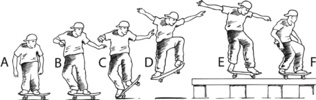
\includegraphics[width = 0.45\textwidth]{figure/f_ollie.png}
        \caption*{\centering \footnotesize Source: \cite{frederick_biomechanics_2006}}
        \caption[Ollie phases]{\footnotesize{(A)`Preparation': athlete lowers their centre of mass(COM) prepares muscles for upward acceleration. \\
        (B) `Pre-pop': skateboard rotates about it's wheels due to force of back foot. \\
        (C) `Pop': tail of the skateboard hits the ground. Skater takes advantage of the collision between the skateboard and ground to bring the skateboard up. \\
        (D) `Upward motion': the skater and skateboard are both airborne. \\
        (E) `Downward motion': the legs are extended to ensure a firm landing. \\
        (F) `Landing': the skater absorbs the impact. }}
        \label{fig:ollie}
\end{figure}

\begin{table}[b]
\begin{center} \label{table:dimensions}
\begin{tabular}{||c c||} 
 \hline
 Variable & Dimension range \\ [0.5ex] 
 \hline\hline
 Kick tail angle & 10-25 [deg]\\ 
 \hline
 Wheelbase & 0.30-0.50 [m]\\
 \hline
 Wheel diameter  & 48-60 [mm] \\
 \hline
 Truck height & 48-56 [mm] \\ 
 \hline
 Tail/nose length & 0.10-0.20[m] \\
 \hline
 Overall length & 0.74-0.85[m] \\
 \hline 
 Deck width& 0.19-0.22 [m] \\ [1ex] 
 \hline
\end{tabular}
\end{center}
    \caption[Typical dimension of a skateboard]{\centering Typical dimensions of a skateboard}
    \caption*{\centering \footnotesize Source: \cite{berger_handmade_2021}}
    \label{tab:dimensions}
\end{table}

Skaters know and feel when a specific skateboard performs to their liking. Though, they don’t know what dimensions support their performance. The skateboard might have evolved to an optimum throughout the years, but from an academical and mechanical point of view, skateboard design has not been proven optimal for specific tricks.

Some researches have tackled this problem by analyzing the skateboard in a planar riding model \cite{hubbard_lateral_1979,hubbard_human_1980,kremnev_nonlinear_2010,ispolov_skateboard_1996,rosatello_skateboard_2015,varszegi_stability_2017,varszegi_stabilizing_2016,varszegi_downhill_2016,varszegi_balancing_2014,kuleshov_mathematical_2007,kuleshov_various_2010}. Which has given insight in the dimensions and stability of rolling and turning. Researchers found that the stability of the skater with skateboard is dependent on the location, and input of the athlete, wheelbase, torsional spring stiffness of roll and forward speed \cite{varszegi_stability_2017,kremnev_nonlinear_2010,hubbard_lateral_1979}. These dimensional analyses don't apply to ollies. Others researched the ollie by investigating the contact forces \cite{anderson_ollie_2020,shield_contact-implicit_2022} and biomechanics \cite{frederick_biomechanics_2006,vorlicek_analysis_2015,wood_3d_2020,nakashima_simulation_2021,nevitt_ground_2006,candotti_lower_2012,dias_using_2016,anderson_ollie_2020,bridgman_human_1992,ou_postural_2021}. Two papers investigated the optimization of the ollie without changing the geometry \cite{anderson_ollie_2020,shield_contact-implicit_2022}. But research does not provide how the skateboards' dimensions influence the ollie. The skateboard community would benefit from knowing how the dimensions of the skateboard influence the performance of the ollie. 
Now that skateboarding joined the Olympics, knowing how to improve performance is more important then ever. The most concrete (i.e. criteria with physical measurement) Olympic judging criteria that applies to the ollie is height \cite{world_skate_skateboarding_2021}. I have parameterized the geometry and inertia characteristics of a skateboard modeled as a single rigid body with parameters: tail length, tail angle, deck length, truck height, and wheel radius. This is an appropriate parameterization for a skateboard designer because the width of the skateboard is usually chosen by preference. Also, the ollie is a movement that involves rotation in one plane, visible in fig. \ref{f_olliesteps}, which means only the inertia characteristics for this rotation are necessary. 
\newpage
\noindent This leads to the following research question:

\begin{quote}
\textit{
    What are the optimal geometric and inertial parameters of a skateboard for an Olympic athlete to reach maximal ollie height?}
\end{quote}

This paper aims to provide information to skaters on how the dimensions of the skateboard influence the ollie.\\ 

\vspace{-1cm}
\section{Method}
\noindent The chosen method to answer the research question is to find the optimal dimensions through optimization. Optimization in sports is helpful for finding optima in control and parameters \cite{ackermann_optimality_2010}. The steps that need to be taken to solve the optimization problem are:
\begin{enumerate}
    \item Understanding the Mechanics of the ollie through literature and a video analysis
    \item Optimal control problem and parameter optimization
    \item Implementing the mechanics into the optimization
    \item Solve the optimization problem for the dimensions of the skateboard for maximum ollie height. 
\end{enumerate}

Before I start with the analysis, I will explain all terminology of the parts of the skateboard. All parts are described with figure \ref{f_skateterminology}. The tail is the inclined part with a rounded top. The nose is the mirrored part on the other side of the skateboard. The tail inclination is with respect to the deck. The kink between the deck and the tail or nose is called the pocket. The deck in skateboard terminology is referred to the tail, nose and the part in between. Though, in this paper the deck refers exclusively to the indicated part in figure \ref{f_skateterminology}. Two trucks connect the wheels to the axles with ball bearings. The top of the skateboard is covered with a sandpaper-like sticker called grip-tape (black part). Concave is the radius of the deck. All pictures in this paper will refer to the front as the right hand side of the skateboard and the back as the left hand side. A riding direction is assumed to be positive right. This convention is chosen because left and right are ambiguous in skateboard terminology as the front foot can be either the right or left leg depending on the stance (goofy, regular respectively). 
\begin{figure}[b]
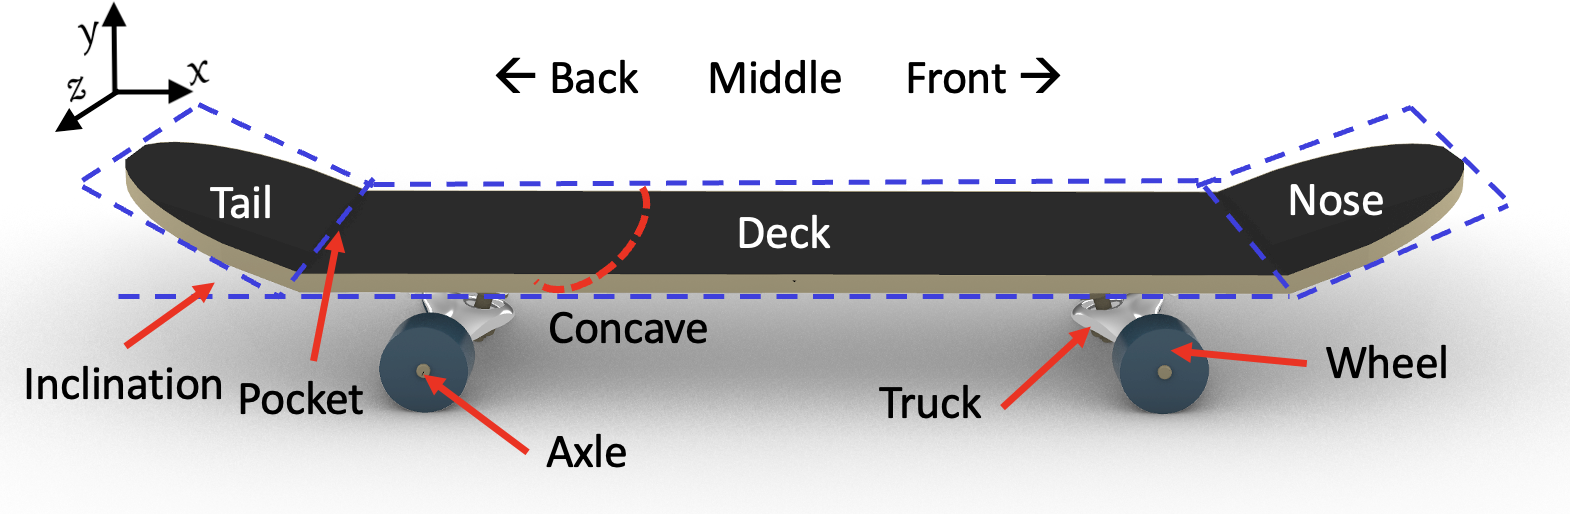
\includegraphics[width=0.5\textwidth]{figure/terminology.png}
\caption[Skateboard terminology]{Skateboard terminology}
\label{f_skateterminology}
\end{figure}

\subsection{Mechanics of the ollie} \label{ss_mechanics}
%%%%%%%%%%%%%%%% begin figure %%%%%%%%%%%%%%%%%%%
\begin{figure}[b]
\subfloat[Vertical ground reaction force]{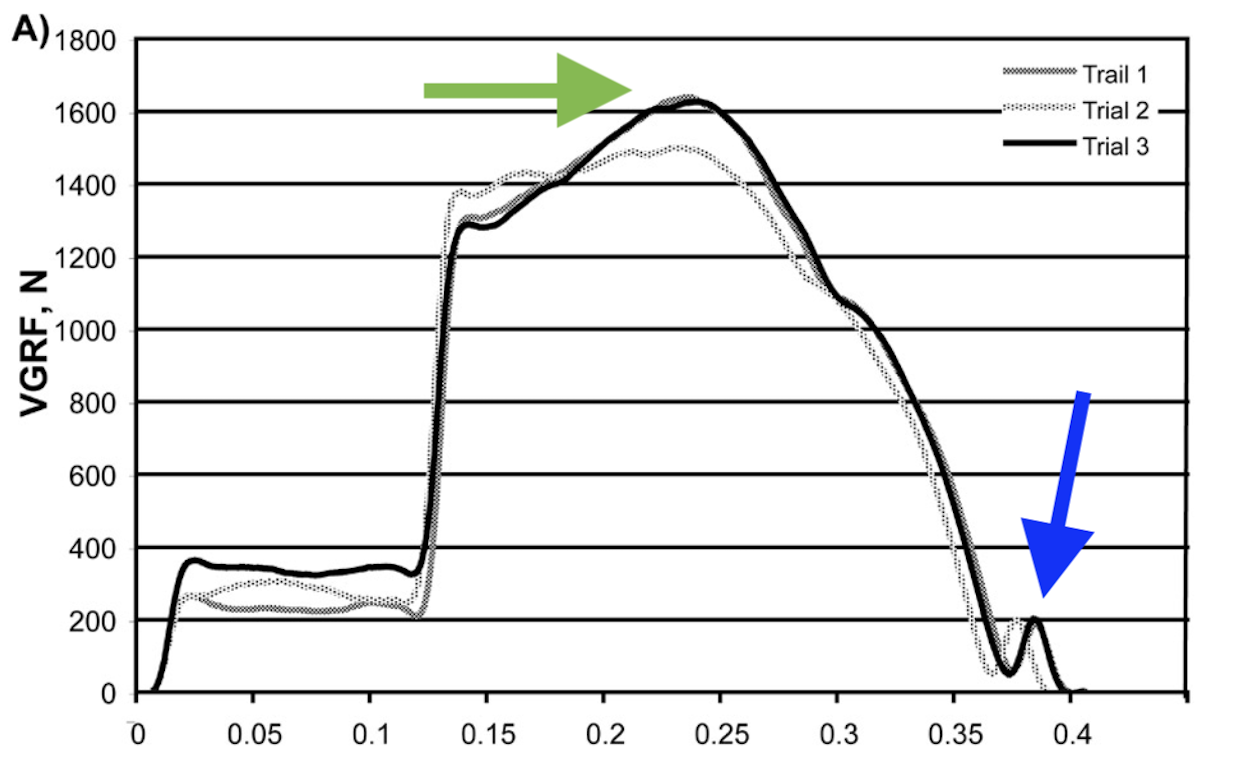
\includegraphics[width=0.25\textwidth]{figure/GRF1.png}}
\subfloat[Horizontal ground reaction force]{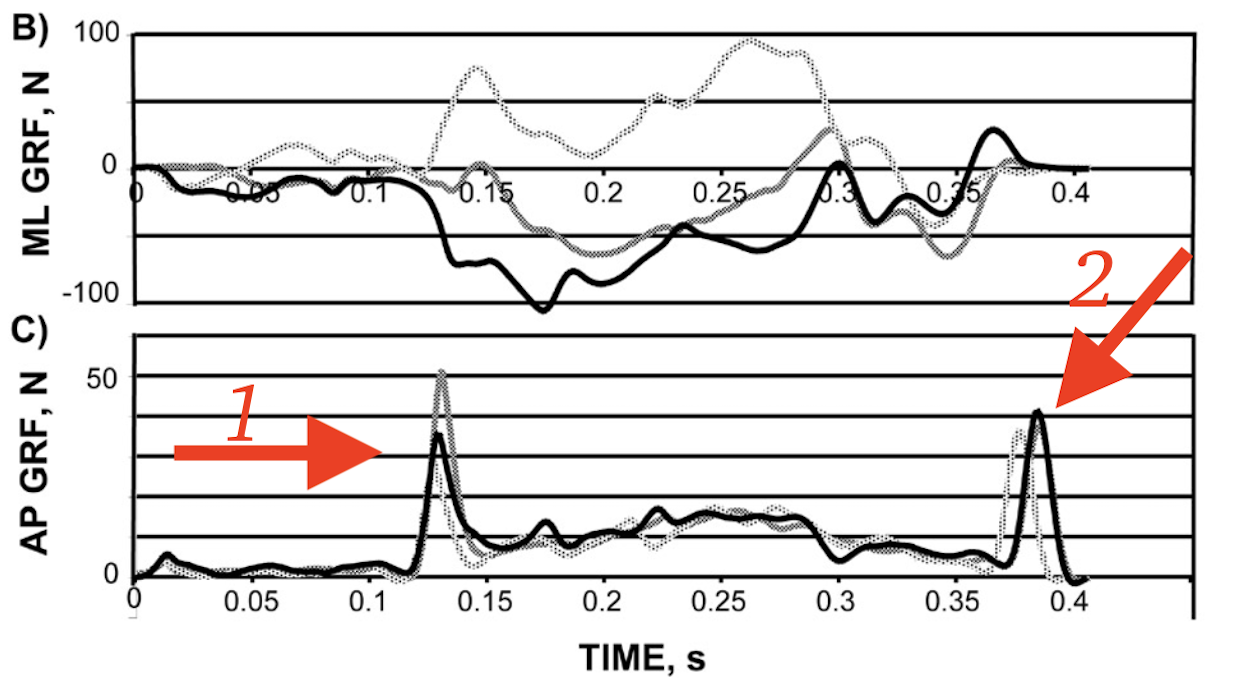
\includegraphics[width=0.25\textwidth]{figure/GRF2.png}}
\caption[Ollie ground reaction force]{Take-off ground reaction forces of the ollie. The green arrow is the highest peak, the blue arrow is the skateboard hitting the ground, the red arrows are friction peaks due to a hard push and tail impact respectively\cite{frederick_biomechanics_2006}}
\label{f_GRF}
\end{figure}
%%%%%%%%%%%%%%%% end figure %%%%%%%%%%%%%%%%%%%

\begin{figure*}[t]
\captionsetup[subfigure]{labelformat=empty}
    \subfloat[$t_1$=0.013]{{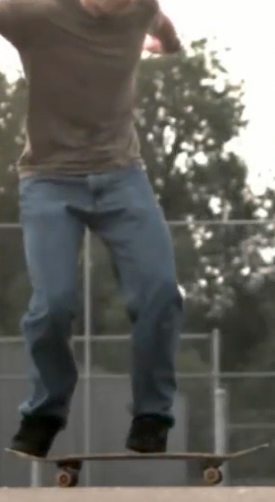
\includegraphics[width=0.13\textwidth]{figure/1.png} }}%
    \subfloat[$t_2$=0.129]{{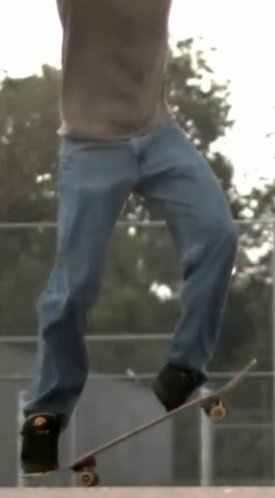
\includegraphics[width=0.13\textwidth]{figure/2.png} }}%
    \subfloat[$t_3$=0.181]{{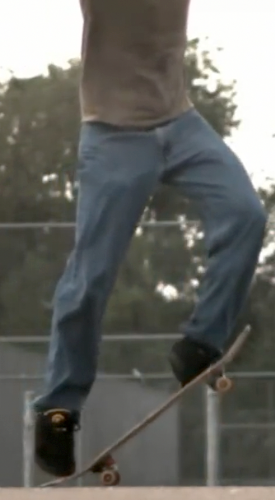
\includegraphics[width=0.13\textwidth]{figure/3.png} }}%
    \subfloat[$t_4$=0.187]{{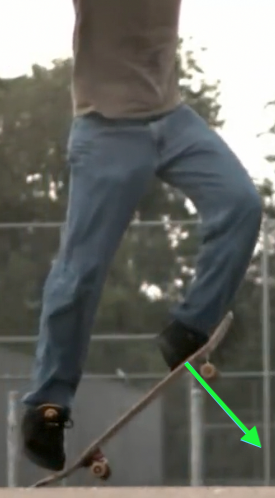
\includegraphics[width=0.13\textwidth]{figure/4.png} }}%
    \subfloat[$t_5$=0.303]{{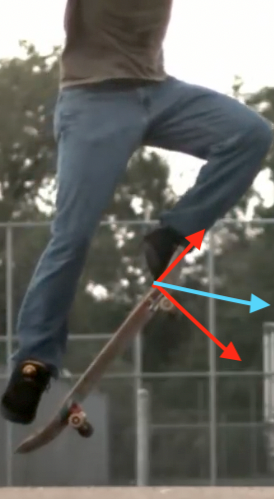
\includegraphics[width=0.13\textwidth]{figure/5.png} }}%
    \subfloat[$t_6$=0.431]{{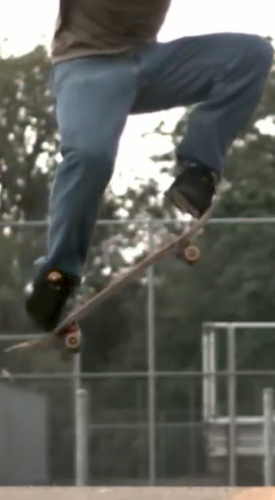
\includegraphics[width=0.13\textwidth]{figure/6.png} }}%
    \subfloat[$t_7$=0.543]{{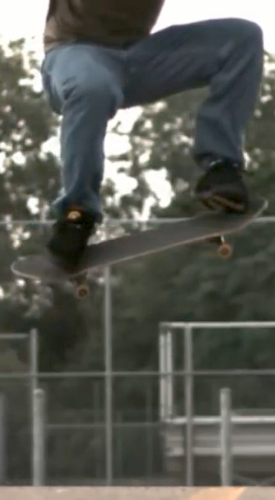
\includegraphics[width=0.13\textwidth]{figure/7.png} }}%
    \protect\newline
    \centering
    \subfloat[$t_8$=0.676$^1$]{{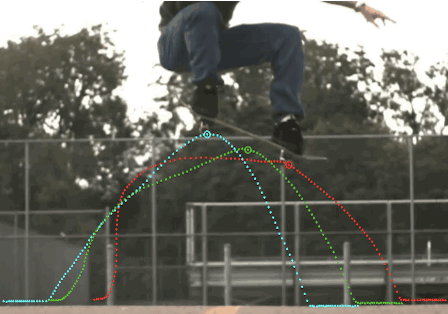
\includegraphics[width=0.336\textwidth]{figure/ollie_tracking_mid.png} }}
    \subfloat[$t_9$=0.722]{{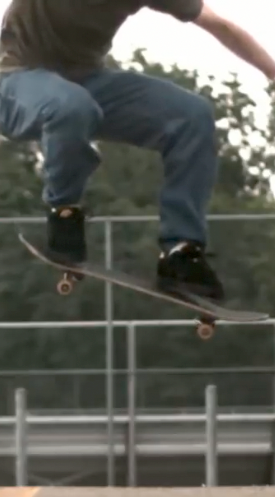
\includegraphics[width=0.13\textwidth]{figure/9.png} }}%
    \subfloat[$t_{10}$=0.904]{{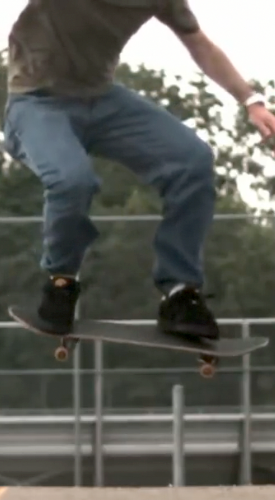
\includegraphics[width=0.13\textwidth]{figure/10.png} }}%
    \subfloat[$t_{11}$=1.097]{{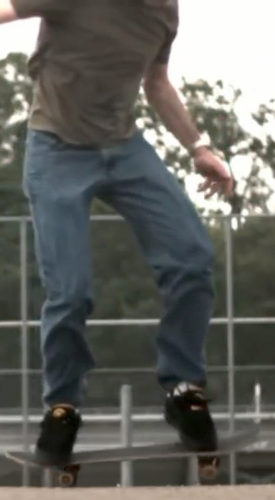
\includegraphics[width=0.13\textwidth]{figure/11.png} }}%
    \captionsetup{singlelinecheck=off}
    
    \vspace{-0.2cm}\caption[Ollie motion cues]{Green arrow: resultant force without friction, red arrows: force components whith friction, blue arrow: resultant force with friction. Blue-, green- and red line are trajectory of back wheel, middle and front wheel respectively\footnotesize\begin{itemize}
    \item[$t_1$] The skater is pushing firmly from his back leg and is starting to have less force on the front foot which results in the wheel just leaving the ground.
    \item[$t_2$] The front foot starts sliding relative to the board for the first time.
    \item[$t_3$] Tail collides with the ground, the front foot is still sliding and the back foot is barely in contact with the skateboard. 
    \item[$t_4$] Back foot is no longer in contact with the skateboard, the back wheels are not in contact with the ground anymore.
    \item[$t_5$] The front foot reached the nose of the skateboard.
    \item[$t_6$] Back foot contacts the board again.
    \item[$t_7$] Board is leveled out by the front foot.
    \item[$t_8$] Highest point is reached. Knees are fully tucked in. Feet are firmly placed on the deck. 
    \item[$t_9$] Front foot loses contact.
    \item[$t_{10}$] Board is horizontal, both feet are in contact.
    \item[$t_{11}$] The back wheels touch the ground and legs are almost fully streched out.
    \item[$^1$] \url{https://www.wired.com/2014/10/skateboard-physics-empzeal}
    \item[$^2$] \url{https://www.youtube.com/watch?v=339k4XEvbxY}
\end{itemize}}
    \label{f_olliesteps}
\end{figure*}

\noindent To understand the mechanics of the ollie, I analyzed a video to find motion cues during the ollie. The video was shot with a Redlake N3 high speed camera at 1000 fps and played back at 60 fps, the time of the events is calculated by taking the time in the video-editor and multiplying it by 1000/60. In a video editor the exact times are noted and a screenshot is taken whenever a distinct motion cue was observed. These motion cues ($t_1-t_{11}$) are given in figure \ref{f_olliesteps}. 

From the video it is clear that both feet can be in contact or not in contact with the board. The collision of the tail with the ground is only applied to the skateboard. The athlete is barely in contact with the skateboard and has already jumped when impact occurs. This is not interpreted in the findings of Fredericks et al. \cite{frederick_biomechanics_2006}. It is stated that the ground reaction force is typically described by a high magnitude peak due to the back foot pushing to the tail and slamming the tail into the ground (see figure \ref{f_GRF} green arrow). Though, after the large peak there is a tiny peak (blue arrow). This peak corresponds to the skateboard hitting the ground. The centre of mass (COM) of the human is already moving upwards and only the skateboard collides with the ground, not the skater. This same tiny peak is found when performing a kick-flip, a similar movement to the ollie but with a rotation about the x-axis(see figure \ref{f_skateterminology} for convention) \cite{determan_kinetics_2006}. 

This is confirmed in a paper by Nakashima \cite{nakashima_simulation_2021} stating that both feet should separate from the deck before the tail of the deck hits the ground. He also stated that the rotational velocity is mostly responsible for the skateboards' upward motion. When creating enough momentum about the rear axle, the rotational speed will provide an upward acceleration. 

The frictional forces seen in figure \ref{f_GRF} (red arrows) also suggest that the small peak is due to the impact of the skateboard. The ollie during the ground reaction force of figure \ref{f_GRF} was performed with a horizontal velocity resulting in a frictional contact of the tail scraping on the ground. When the tail hits the ground, friction should increase on the force plate. The only moment that friction increases is when a hard downward push creates an increase in rolling resistance (red arrow 1), and when the tail hits the ground (red arrow 2). The force is already below 200 [N] at that time instance, meaning that the human is either already airborne or about to be airborne.

Friction is not only seen during the impact, but also between the feet and the griptape. Due to the normal force perpendicular to the board together with a friction force tangential to the surface, the resultant force will take the form of a similar nature as shown in figure \ref{f_olliesteps}, $t_5$. If no friction would be present during this contact the resultant force would point more down as shown in $t_4$, resulting in a lower ollie. The higher the coefficient of friction between the foot and the deck, the more up the resultant force will be. And lastly it can be concluded that the bio mechanical obstruction of the feet cause the skateboard to not go further up. The knees are fully tucked in at the highest point, the skateboard can't go higher through this physical bound. 

A real skateboard bends and flexes during the ollie, but I decide to assume an rigid body model of the skateboard because of the increased complexity. Also, bending is a source of energy dissipation in addition to the energy loss due to local deformation \cite{stronge_impact_2000}. This suggests that an infinitely stiff board would dissipate the least energy, which would result in the highest ollies. On the other hand flexure of the board could serve as an energy storage for the human that could not have been used otherwise. For example in snowboarding, the flexure is used to gain upward momentum. In this paper flexure is not taken into account and could be an interesting topic for future researchers.


\newpage
\subsection{Introduction to the Optimal Control Problem}
\noindent To optimize the ollie and the geometry of the skateboard, the observations from the previous section should be modeled numerically with physics and mathematics. Before the physical ollie phenomena are discussed, the chosen optimization scheme is introduced. 

\subsubsection{Optimal Control}\label{s_optimalcontrol}
\noindent There are three types of optimizations to solve an optimal control problem (OCP) \cite{kelly_transcription_2017}:
\begin{itemize}
    \item \textbf{Dynamic programming} - This type of optimization discretizes the whole solution space and finds the global optimum. A perfect method for a low dimensional system. But when scaling to a high dimensional system the computation time will increase exponentially. 
    \item \textbf{Indirect methods} - Transcribe the problem and find where the slope of the objective is zero. Often numerically unstable and difficult to implement and initialize.
    \item \textbf{Direct methods} - Transcribe the problem then find the minimum of the objective function. Can transcribe well to high dimensional systems, but is prone to finding a local optima because it searches a single trajectory through state and control space rather than a global method like dynamic programming.
\end{itemize}
I chose the direct method, because direct methods are generally best for problems where dynamics and control must be computed to a similar accuracy, and the structure of the control trajectory is not known a priori \cite{kelly_introduction_2017}. Also, the ollie is highly non-linear and complex movement with high dimensionality . With this method it is possible to increase the dimensionality without increasing the difficulty to solve the optimization. 

\subsubsection{Transcription and Mesh}
\noindent Transcription is converting a continuous problem into a non-linear programming problem (NLP). There are shooting methods and simultaneous methods. A shooting method uses a simulation to enforce the system dynamics, while the simultaneous method enforces the dynamics at given points along the trajectory. The chosen method is a simultaneous method called orthogonal collocation. The software that is used is called PyCollo, which is direct orthogonal collocation transcription tool for Python \cite{brockie_predictive_nodate}. The dynamics and constraints are enforced over a discretization. The discretization exists of $N$ collocation points. The collocation points are either mesh points or polynomial points, but all collocation points are enforced to the constraints and dynamics. After transcription the problem is passed to the solver IPOPT (Interior Point OPTimizer). When the found IPOPT solution does not meet the error-tolerance set in PyCollo, the discretization is refined and a new iteration is solved in IPOPT. Mesh points, polynomial points, mesh sections and mesh refinement are explained in figure \ref{f_phmesh}. The polynomials are of the Legendre-Gauss-Lobatto (LGL) nature. More information on the mesh can be found in appendix A. The integration scheme is an implicit Runge-Kutta Kth method \cite{brockie_predictive_nodate}. This high order method will have a high accuracy with the disadvantage that all states and constraints need to be differentiable.

\begin{figure}
    \centering
    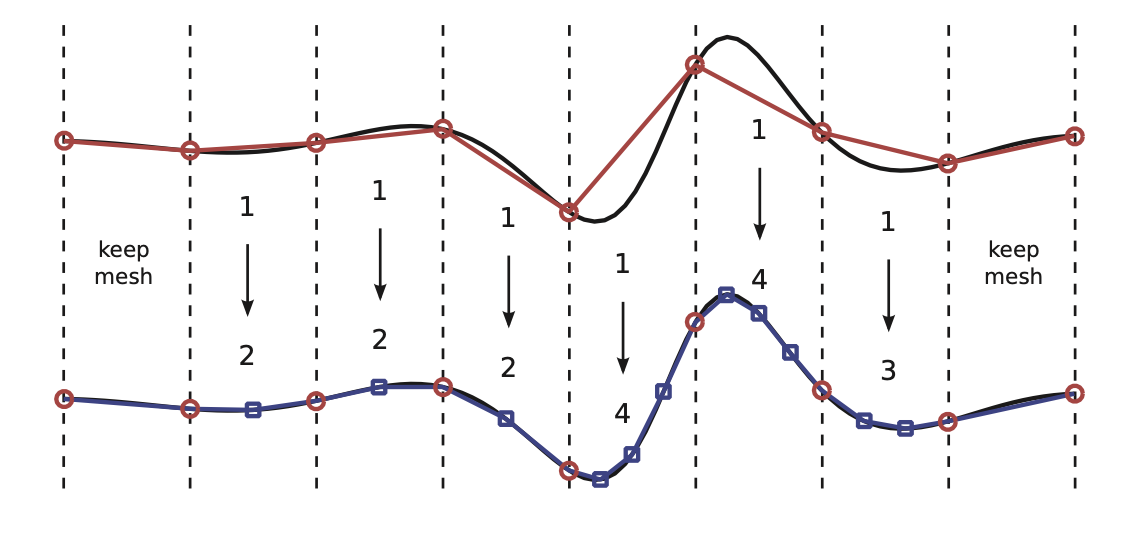
\includegraphics[width = 0.5\textwidth]{figure/phmesh.png}
    \caption[Mesh section and polynomials]{Mesh sections are indicated with the dotted vertical lines. The first line shows an optimization solution (red line) that has an error from the true solution (black line). With the increase of polynomial points the mesh is refined and the solution is better after a new iteration into IPOPT. If polynomial points exceed the limit of 10 points per mesh section, the mesh section will be made smaller. Highly nonlinear sections will refine more giving an efficient computation}
    \footnotesize Source: \cite{kelly_introduction_2017}
    \label{f_phmesh}
\end{figure}

\subsubsection{Hybrid problem}
\noindent The ollie problem is a hybrid problem, meaning that there will be discontinuities in the states. For example during impact the velocity states change sign instantly causing discontinuities. Discontinuities are per definition not differentiable, this means that in a higher order optimization the discontinuity need to be solved differently. The chosen method is to implement a multi-phase optimization. Multi-phase optimization concerns a sequence of continuous-state phases separated by discrete jumps in the states. Multi-phase optimization requires pre-modeled phases which leaves no opportunity for unsought solutions. Though, they are easier to compute and tend to be more accurate \cite{kelly_introduction_2017}. Since the impact is prescribed in the ollie, solving the impact velocities discretely will provide an accurate solution.

% The mechanics of the ollie show discontinuous behaviour, such as impact and friction. This usually leads to bad convergence for the solver. The solution is to change the system dynamics. For example, to discribe discontinous phenomena as continuous or split the problem up in several phases that are fully continuous or a combination of both. Impact can be solved with through-contact optimization. This is a continuous approximation of impact where contact mechanics are modeled with spring damper models.  The friction contact is not known in the ollie problem and can change throughout the whole movement. This is why a continuous approximation is chosen for the friction shown by equation \ref{e_friction}.
\subsection{Parameter optimization}\label{s_paropt}
\noindent In section \ref{s_optimalcontrol} it was made clear that with the chosen method increasing the dimensionality of the problem is feasible. The skateboards' parameters can be optimized as decision variables which increases the state space, but with direct methods this should not be a problem. It is similar to setting an initial value of a state free for optimization but now it will be a parameter defining the skateboards geometry. To optimize the geometry of the skateboard I made a parameterized model of the skateboard that scales it's mass and inertia values when changing the geometry, such that the dynamical response is scaled as well. I used the SymPy symbolic toolbox to create the parameterized models \cite{meurer_sympy_2017}. 

\subsubsection{Parameterized model}\label{ss_model}
%%%%%%%%%%%%%%%% begin figure %%%%%%%%%%%%%%%%%%%
\begin{figure}
\centerline{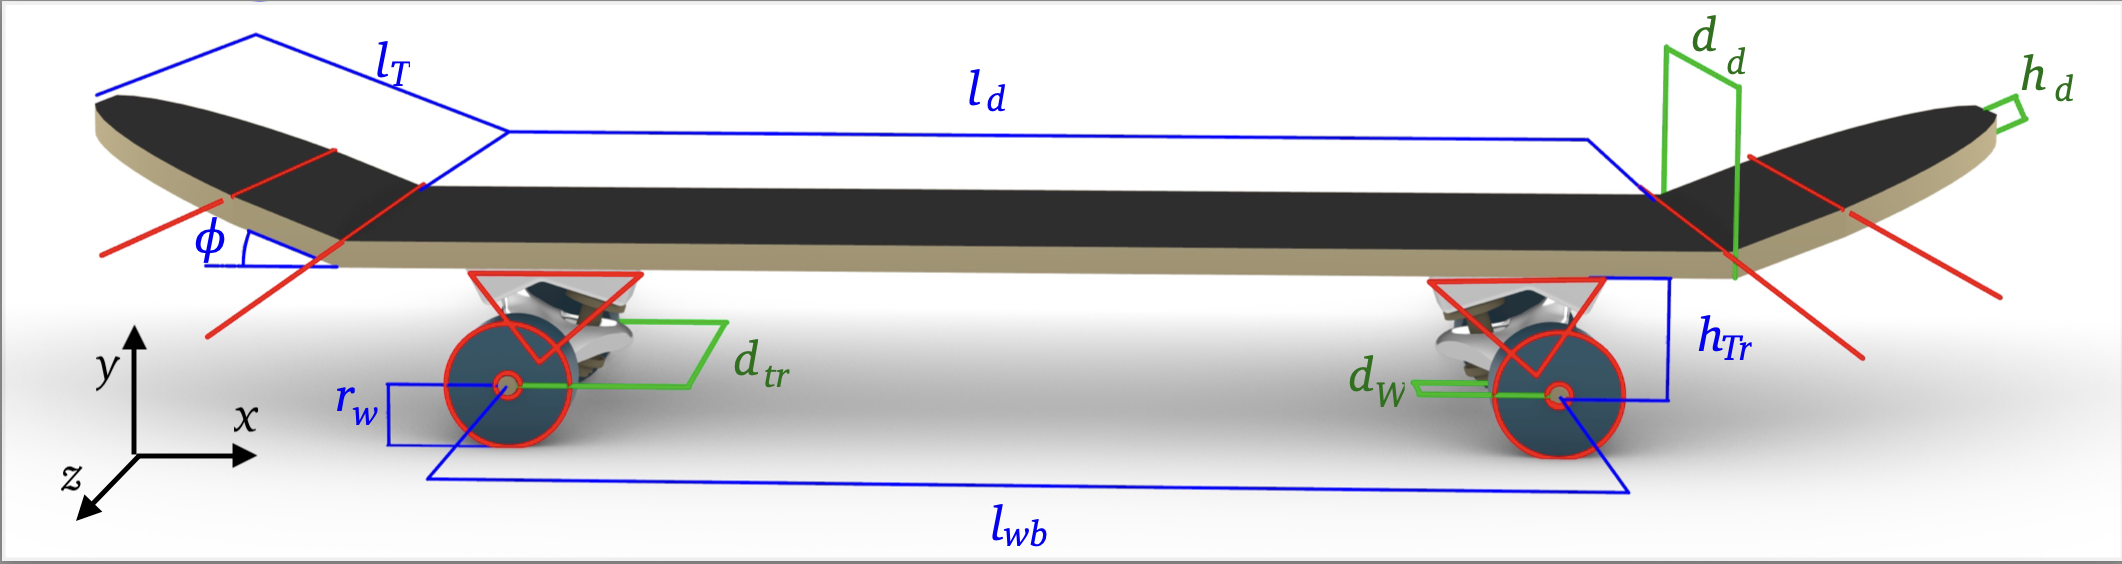
\includegraphics[width=0.5\textwidth,trim={0.1cm 0.1cm 0.1cm 0.05cm},clip]{figure/parameterized.png}}
\caption[11-Segment skateboard model]{Parameterized skateboard. Blue variables are located in the xy-plane. All blue variables except for $h_d$ and $d_{com}$ are optimized during the ollie optimization. Green variables are chosen by preference. Red lines split the skateboard into 11 basic shaped segments for inertia calculation (see figure \ref{f_basicshapes})}
\label{f_11segments}
\end{figure}
%%%%%%%%%%%%%%%% end figure %%%%%%%%%%%%%%%%%%%

\noindent The most widely accepted skateboard is the Popsicle stick skateboard (see section \ref{s_intro}). A simplification of the Popsicle stick skateboard is minimally described in ten variables. A symmetrical shape is assumed, whereas in reality nose and tail length and inclination often vary. The simplified skateboard is made up of straight lines only and concavity is not taken into account. An infinitely stiff skateboard is assumed as stated in section \ref{ss_mechanics}. Eight variables are located in the xy-plane shown in blue in fig.\ref{f_11segments}. Wheelbase ($l_{wb}$), deck length ($l_{d}$), length tail and nose ($l_{t}$), tail and nose inclination relative to the deck ($\phi$), truck height ($h_{tr}$), wheel radius ($r_{w}$), and COM distance from deck $d_{com}$. These will be the optimization variables because they affect the 2D kinematics of the ollie directly, except for $d_{com}$. As $d_{com}$ is a function of the other parameters. All other parameters are set at the industry standard or a measured value (see table \ref{t_typical}). Deck thickness ($h_d$) is dependent on the amount of layers of veneer that is used during production. All zx-plane related variables are shown in green in fig.\ref{f_11segments}. Truck width ($d_{tr}$), and wheel width ($d_w$), deck width ($d_d$). They are usually chosen by the skater through preference and won't be part of the optimization. Truck and deck width are assumed to be equal. This leads to the variables that will be optimized for improving the geometry of the skateboard during an ollie:
\begin{equation}
    [l_{wb},\ l_d,\ l_t,\ \phi,\ h_{tr},\ r_w ]
\end{equation}

\subsubsection{Mass distribution}\label{ss_mass}
\noindent The mass and it's distribution influence the dynamic response of the skateboard \cite{moore_force_nodate}. A mass model is made to be able to scale the mass and it's distribution when the optimized parameters are changed. The skateboards' COM is calculated as a composite of 11 basic constant density shapes shown in figure \ref{f_basicshapes}. The shapes consist of semi-cylinders, cuboids, cylinders and triangular prisms. To calculate the mass of each part, the volume of each segment is calculated and multiplied by it's density except for the trucks. For the trucks, density is calculated from a measured truck weight divided by the volume of the truck estimated as an triangular prism. The typical weight influencing properties are seen in table \ref{t_typical}. See appendix A for mass, inertia, and geometry calculations. 
\begin{figure}
    \centering
    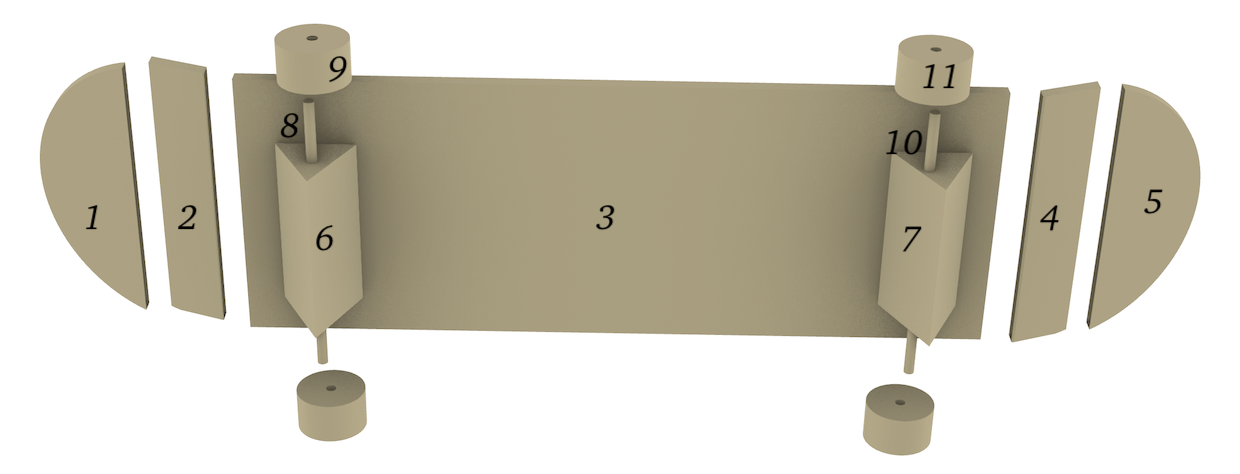
\includegraphics[width = 0.5 \textwidth]{figure/Basicshapes.png}
    \caption[Exploded 11 segment model]{Clarification on the 11 segment model. Now you can see that there are 13 shapes, but the wheels are taken as one wider cylinder in 2D, which results in 11 segments}
    \label{f_basicshapes}
\end{figure}
%%%%%%%%%%%%%%% begin table   %%%%%%%%%%%%%%%%
\begin{table}[t]
\begin{center}
\caption[Industry standard and measured skateboard dimensions]{Industry standards and measured values from a PolarSkate Co. deck with Independent trucks}
\label{t_typical}
\begin{tabular}{l l l}
& & \\ % put some space after the caption
\hline
Description & Variable & Value \\
\hline
Wheel density (PU) & $\rho_{pu}$    & $1130 \quad [\frac{kg}{m^3}]$ \footnotemark\\
Hard maple density & $\rho_{maple}$ & $705 \quad [\frac{kg}{m^3}]$ \footnotemark\\
Thickness veneer & $d_{veneer}$ & $0.0016 \quad [m]$ \footnotemark\\
Specific mass PVA glue & $s_{glues}$ & $0.105 \quad [\frac{kg}{m^2}]$ $^{3}$  \footnotemark  \\
Density steel & $\rho_{steel} $ & $ 7700 \quad [\frac{kg}{m^3}] $ \\
Radius axle & $r_{axle} $   & $0.004 \quad [m] ^*$ \\
Width deck & $d_{D}$ & $0.21 \quad [m] ^*$ \\
Number of ply's & $n_{ply}$  & $7 $ \\
Mass bearing & $m_{bearing} $ & $0.012 \quad [kg] ^*$ \\ 
Mass truck   & $m_{truck} $   & $0.366 \quad [kg] ^*$ \\
\hline
\multicolumn{3}{l}{$^{1}$ \scriptsize{\url{https://www.lorkindustrias.com/}}} \\ \noalign{\vskip -4mm}    
\multicolumn{3}{l}{$^{2}$ \scriptsize{\url{https://www.wood-database.com/hard-maple/}}} \\ \noalign{\vskip -4mm}
\multicolumn{3}{l}{$^{3}$ \scriptsize{\url{https://www.timberaid.com/}}} \\ \noalign{\vskip -4mm}
\multicolumn{3}{l}{$^{4}$ \scriptsize{\url{http://www.franklinadhesivesandpolymers.com}}} \\ \noalign{\vskip -4mm}
\multicolumn{3}{l}{$^{*}$ \scriptsize{Measured with caliper (+-0.1mm) or with scale (+-1gram)}} \\ \noalign{\vskip -4mm}
\end{tabular}
\end{center}
\end{table}
%%%%%%%%%%%%%%%% end table %%%%%%%%%%%%%%%%%%%

%%%%%%%%%%%%%%% begin table   %%%%%%%%%%%%%%%%
\begin{table}
\begin{center}
\caption[Inertia]{Formulas of volume and inertia of each basic shape to calculate skateboards inertia. $l=$ length, $d=$ width, $r=$ radius L = length of isosceles, $\beta$ = top angle of isosceles}
\label{t_volume_inert}
\begin{tabular}{c l p{1.06in}}
& & \\ % put some space after the caption
\hline
Shape & Volume & Inertia \\
\hline
Cuboid           & $l\cdot d\cdot h$              & $\frac{m}{12} (l_x^2+l_y^2)$ \\
Triangular prism & $\frac{1}{2} l\cdot d\cdot h$  &  $\frac{1}{2} m L^2\left(1-\frac{2}{3} \sin ^2 \beta\right)$ \cite{morin_introduction_2008}\\
Cylinder         & $\pi h (R^2-r^2)$                        &  $I_{x},I_{y} = \frac{m}{12} (3 r^2 + l^2)$ $I_{z} = \frac{r^2}{2 m} $ \\
Semi-cylinder    & $\frac{1}{2}\pi h (R^2-r^2)$             &  $(\frac{1}{4}-\frac{16}{9 \pi^2}) m r^2)$ \\
\hline

\end{tabular}

\end{center}
\end{table}
%%%%%%%%%%%%%%%% end table %%%%%%%%%%%%%%%%%%%


\subsubsection{Inertia}\label{ss_inertia}
\noindent To know the dynamic rotational response of the skateboard, the inertia about the skateboards' COM is needed. When the optimized parameters change the inertia should scale accordingly. A simplified inertia is calculated from the basic shapes found in figure \ref{f_11segments}. Inertia's about the COM of each segment can be found in table \ref{t_volume_inert}. The total inertia about the COM of the skateboard is calculated with the parallel axis theorem:

\begin{equation}
    I_{total} = \sum_{i=1}^{11} I_i + m_i  |\vec r_{i/com}| ^2
\end{equation}

\noindent A series of measurements is performed to validate the inertia model. For more detailed information on the inertia model and inertia measurement see Appendix A
% \paragraph{Verification}
% To make sure the theoretical models are valid, the mass en inertia of two arbitrary skateboards are measured. 
% \paragraph{Inertia measurement}
% The moment of inertia of the two skateboards are measured by hanging the parts as a compound pendulum and measuring their periods of oscillation. A similar method has been shown effective by Moore \cite{moore_accurate_2010}.

% For the simulation only the inertia about the COM in the xy-plane is necessary. 

% When considering a compound pendulum in a 2D-plane with friction, the torque acting on the system due to the gravity is:

% \begin{equation} \label{torque}
%     \tau = -L m g sin(\theta) + c L \dot sin(\theta)
% \end{equation}
% Eulers second law of motion with a fixed origin reduces to $\sum M_o = I_o \Ddot \theta $. Assuming small angles \ref{torque} can be written as:
% \begin{equation}
%     \Ddot \theta I_o = -L m g \theta + c L \dot sin(\theta)
% \end{equation}

% Pendulum
% How measurement is done


\subsection{Multi-phase Direct Collocation}\label{s_multiphase}
\noindent Provided the framework to perform a parameter optimization that scales mass and inertial values accordingly, the ollie optimal control problem should be set up next. Section \ref{s_multiphase} will show the method of modeling the ollie phenomena as well as the implementation within the optimization.

\newpage
\subsubsection{General formulation}
\noindent The multi-phase OCP with phases $p \in [1,2,3]$ involves determining the states $\mathbf{q^{(p)}}$, control $u^{(p)}$, phase initial times $t_0^{(p)}$, final times $t_F^{(p)}$, global parameter variables $\sigma$, while maximizing the objective function:
\begin{equation}
    maximize\ \mathcal{J}
\end{equation} 
Subject to the dynamical constraints:
\begin{equation}
\ddot{\mathbf{q}}^{(p)}=\alpha^{(p)}
\end{equation}
with path constraints,
\begin{equation}
        \gamma^{(p)}:\quad \gamma_{min} < ... < \gamma_{max}\\
\end{equation}
and with endpoint constraints:
\begin{equation}
    \beta:\quad \beta_{min} < ... < \beta_{max}
\end{equation}
The ollie OCP will be explained in the order of equations (2-5). Starting with the choice of phases and objective ($\mathcal{J}$). Then describing the dynamic constraints $\alpha$, consisting of the equations of motion (EOM) for the different phases for the human and the skateboard. Followed by the constraints $\gamma$, where the kinetics and kinematics of the human, and friction are implemented. Then endpoint constraints $\beta$, which contain modeling of impact and the bounding of time. The initial and final state and control values are found in Appendix A and are set to a wide margin. If the margin is not set widely, it will be discussed during these paragraphs. All together, this gives all information necessary to solve the ollie OCP. Section \ref{s_summary} gives a summary of the implementations before starting the results section.

In section \ref{s_paropt} are the geometrical variables described that will be optimized. The wheelbase $l_{wb}$, deck length $l_d$, tail length $l_t$, tail inclination $\phi$, truck height $\h_{tr}$, and wheel radius $r_w$ are set as global parameter variables:
\begin{equation}
\begin{array}{rlrl}
    \sigma_{1} &= l_{wb},\ \sigma_{2} &= l_d,\ \sigma_{3} &= l_t,   \\ 
    \sigma_{4} &= \phi,\ \sigma_{5} &= h_{tr},\  \sigma_{6} &= r_w 
\end{array}
\end{equation}

\subsubsection{Phases and Objective} \label{s_phases}
\noindent The phases of the ollie shown in figure \ref{fig:ollie} in section 1 are \cite{frederick_biomechanics_2006}
\begin{itemize}
    \item[(A)]Preparation
    \item[(B)]Pre-pop
    \item[(C)]Pop
    \item[(D)]Upward motion
    \item[(E)]Downward motion
    \item[(F)]Landing
\end{itemize}
For the purpose of the optimization this has been simplified to three phases:
\begin{enumerate} \label{n_phases}
    \item Preparation phase (A,B)
    \item Upward motion (C,D)
    \item Downward motion (E,F)
\end{enumerate}
\noindent I chose to take A and B as one phase, because the dynamics will not change during these phases. Then the same goes for phase C and D, except that compared to phase 1, the dynamics have changed. The skateboard is now airborne, meaning that there is no ground reaction force any more. Furthermore between phases 1 and 2 discontinuities will occur in the velocity states due to impact. By choosing the phase switch at that specific time instance, the discontinuities can be handled during the switch of the phases, creating a continuous domain over both phases. More on this later in section \ref{p_endpoints}. The end of the second phase is chosen such that the objective function can be described properly. Namely, the objective function of the multi-phase optimization needs to be a function of initial or final state variables \cite{brockie_predictive_nodate}. The objective is to ollie as high as possible, thus by choosing the end of phase 2 to be the highest point of the skateboard, the objective can be expressed in terms of final state variables of phase 2. Because a parameter optimization will occur simultaneously with finding the optimal trajectory, the parameters should not be able to influence the objective. For example, if the objective would be to reach maximum height with the tip of the tail, then the parameter optimization will find maximum tail length, tail inclination, truck height, and wheel radius. Because all these variables influence the height of the tip of the tail. To make sure the objective function is independent of the parameter variables, the skateboard is constrained to be level at the highest point and the objective is the middle of a fictional tangent touching lowest point of both wheels. This result in the objective function:

\begin{equation}
    \mathcal{J} = y_s^{(2)}(t_F) + d_{com} - h_{tr} - r_w 
\end{equation}

Where $y_s^{(2)}(t_F)$ is the final state COM location of the skateboard, $d_{com}$ the skateboards' COM to the deck, $h_{tr}$ the truck height, and $r_w$ is the wheel radius.

\subsubsection{System Dynamics}\label{s_systemdynamics}
\begin{figure}
    \centering
    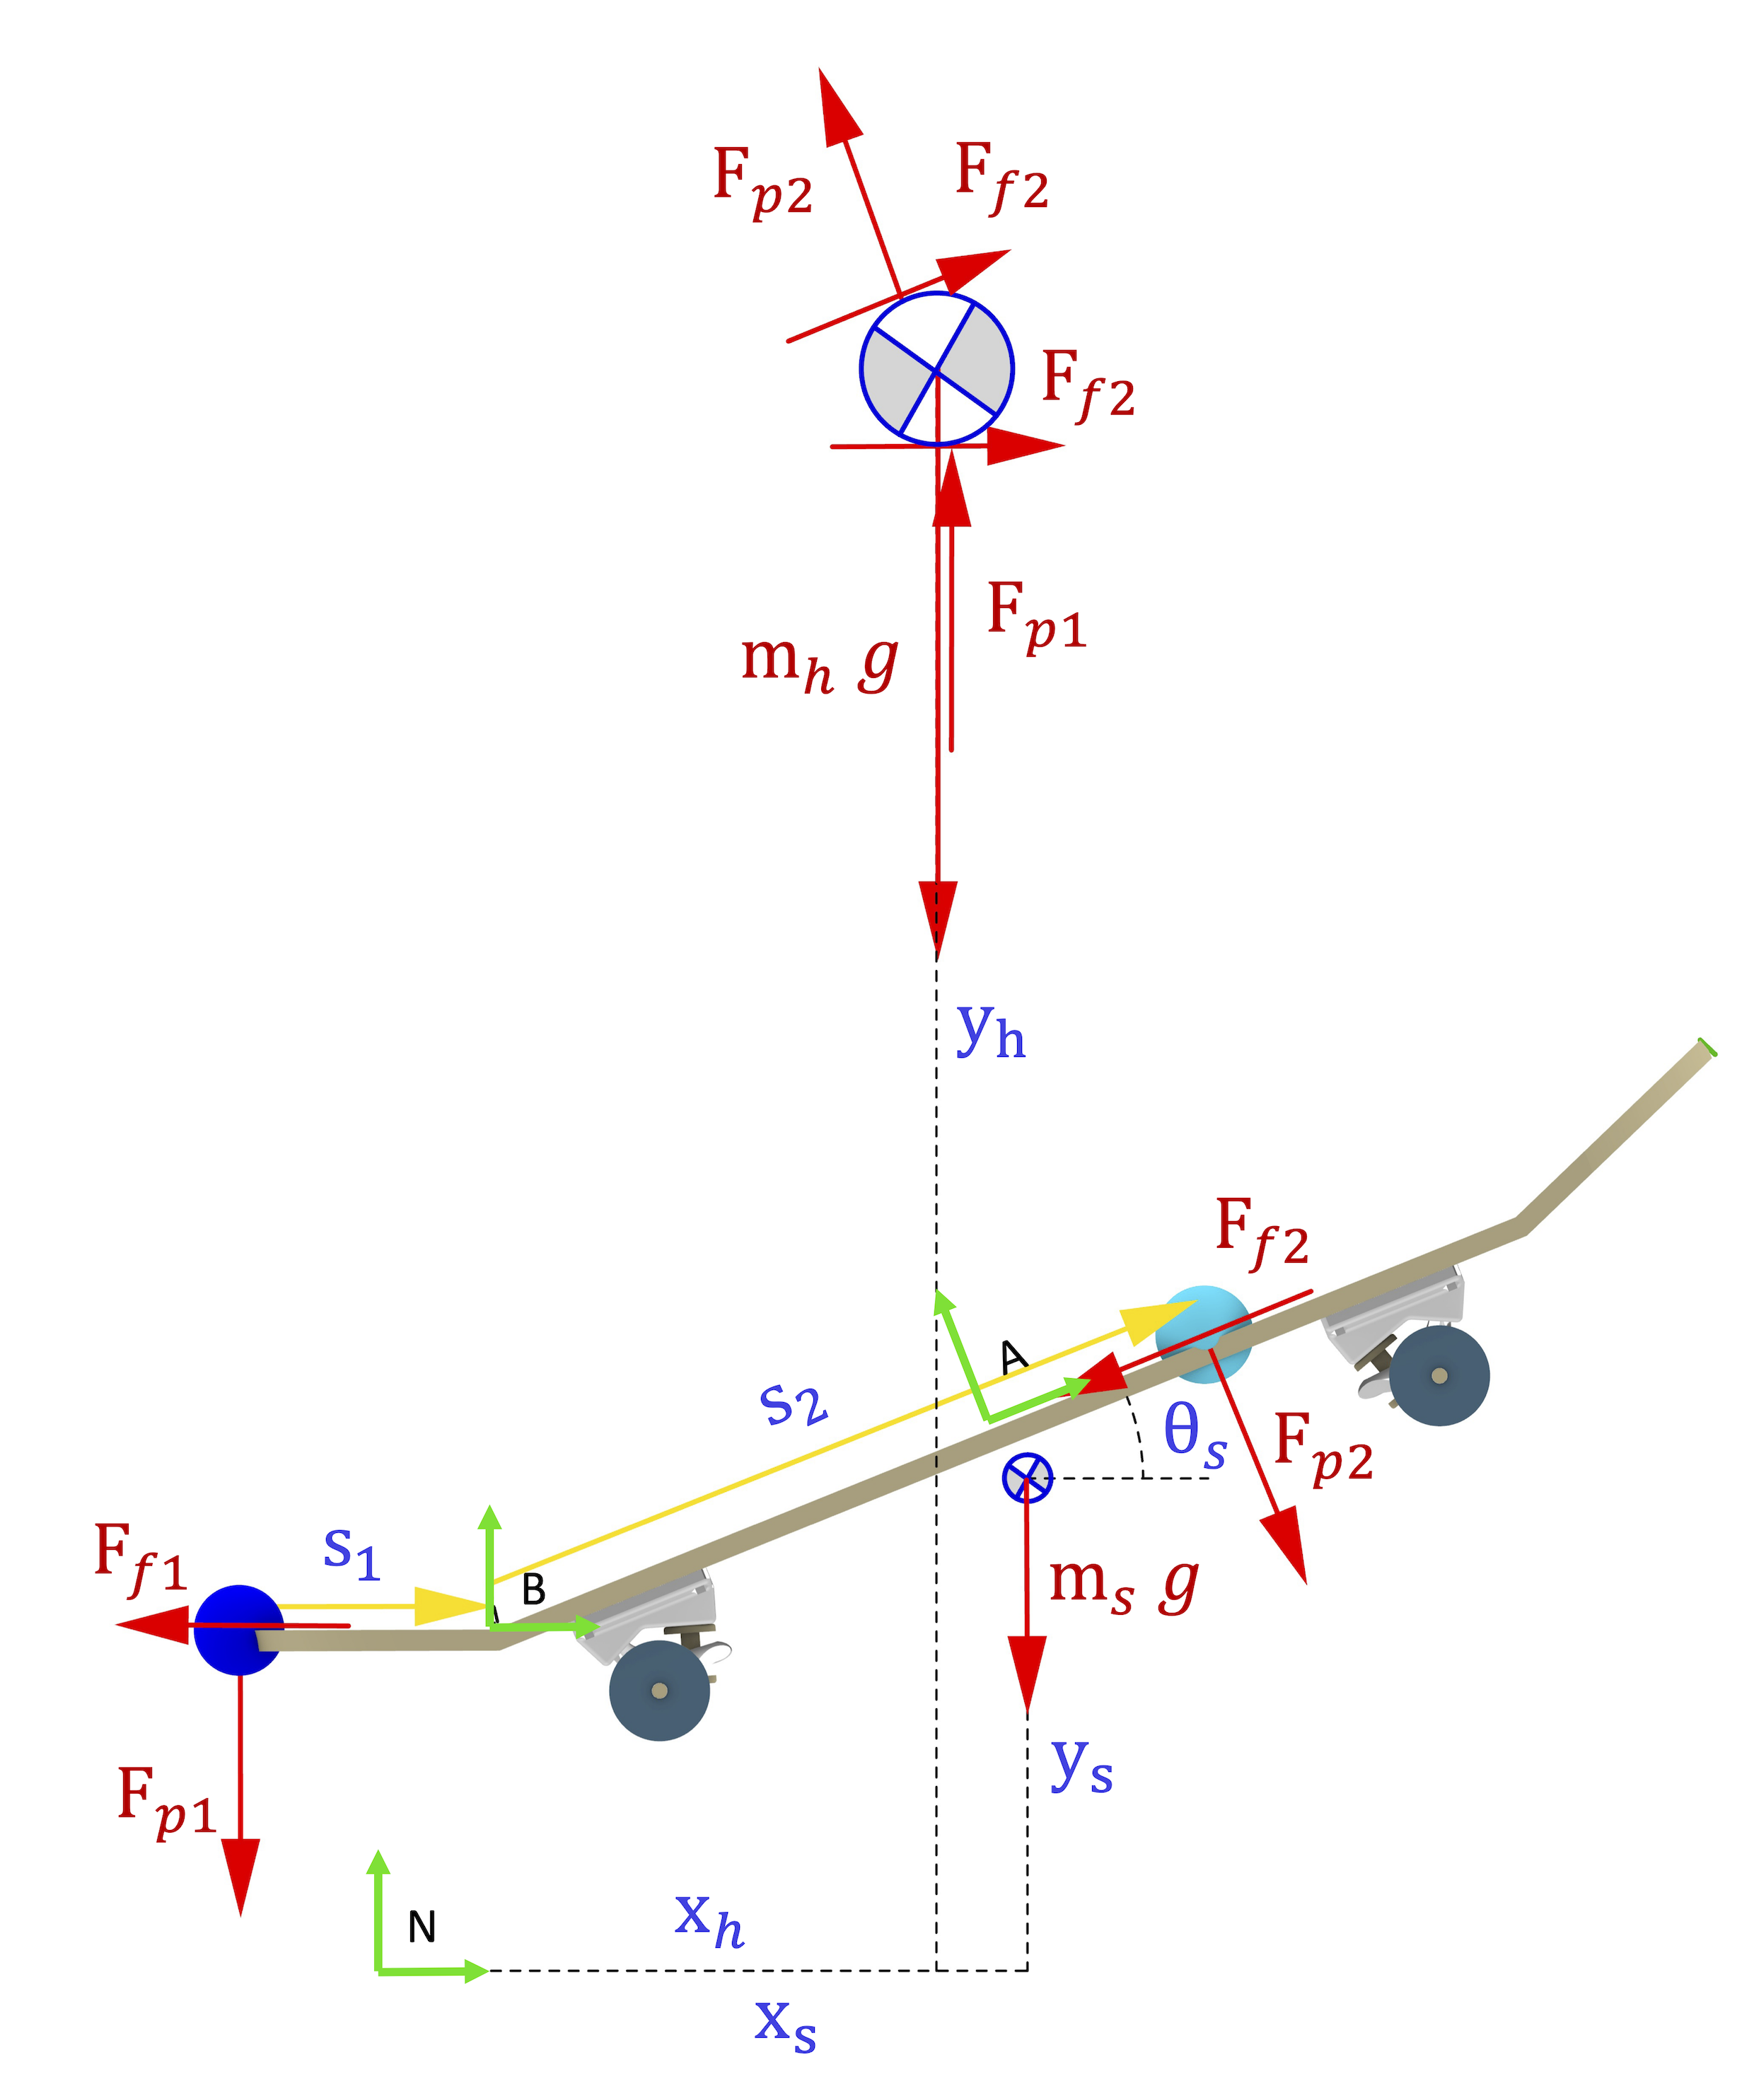
\includegraphics[width=0.45\textwidth]{figure/FBD_skater_feet.png}
    \caption[Free Body Diagrams phase 2 and 3]{Free body diagrams of human and skateboard for phase 1. Blue letters are state variables, Red arrows are forces, the dark blue dot indicates the back foot and the forces that are exerted by the foot. Same goes for the front foot, indicated with a cyan dot. When the foot slides, $s$ is changed and friction will be present. The force exerted by the feet are always perpendicular to the board and can never be negative. Green arrows are frames, N frame is the inertial frame, A and B are body fixed. The forces are equal and opposite acting between the feet and the human centre of mass (top). Skateboard has 3 degrees of freedom, the human has two.}
    \label{f_FBD}
\end{figure}
\noindent The system exists of a point mass (the humans' COM) interacting with a rigid body (skateboard). The interaction between the mass point and the body are simulated with equal and opposite forces acting between the massless feet of the human and the COM of the human. The feet locations can move along the top of the skateboard. In figure \ref{f_FBD} is visible that the forces $F_{p1},F_{p2},F_{f1}$, and $F_{f2}$ are equal and opposite between the feet and the COM. $F_{p1},F_{f2}$ are expressed in the body fixed frame B. $F_{p2},F_{f2}$ are expressed in the body fixed frame A. The perpendicular forces $F_{p1}$, and $F_{p2}$ are positively bound to make sure the feet can never pull perpendicularly on the skateboard. I derived the EOMs using SymPy mechanics and the symbolic toolbox \cite{meurer_sympy_2017}.

\paragraph{Human Equations of Motion}
\noindent I modeled the human as a point mass. The point mass is the COM of a human. The simplification ignores many body segments. Which means this model is not representable in terms of metabolic leg power. Only the mechanical power output can be estimated with this model \cite{van_der_kruk_power_2018}. This is confirmed by Morin in \cite{morin_biomechanics_2018}. With this approximation, inertia of the humans' body and segments is neglected. This is reasonable because during the ollie, the human rotates minimally on top of the skateboard (see figure \ref{f_olliesteps}). The human interacts with the skateboard with forces perpendicular to the skateboard $F_{p1,2}$ and frictional forces tangent to the deck surface ($F_{f1,2}$). These forces are equal and opposite forces between the skateboard and the human as shown in \ref{f_FBD}. The location of these force points are dependent on the location of the feet. The back and front feet are indicated with a blue and cyan dot and are defined on the skateboard with variables $s_1$ and $s_2$ respectively. The kinetics and kinematics of the human will be discussed in the constraint section. The human has two degrees of freedom; $x_h$, and $y_h$. Since the forces on the skateboard are equal and opposite to the human, the EOM are formed from equation \ref{e_Fi} without rotational component and equation \ref{e_newtoneuler} with a different mass matrix $\mathbf{M_h} = [m_h, m_h]^T$ :
The EOMs of the human are found with the Newton Euler equations:
\begin{equation}\label{e_newtoneuler}
\begin{array}{c}
        m_s \cdot \ddot x_s = \sum F_x  \\
        m_s \cdot \ddot y_s = \sum F_y  \\
        I_s \cdot \ddot \theta_s = \sum M_c
    \end{array}
\end{equation}
The forces are expressed in the body fixed frames A, and B. This results in the force of the back foot, force of the front foot and combined the total force acting on the human:
\begin{equation} \label{e_humanforce}
\begin{array}{cc}
      \mathbf{F_{bf}} = F_{p1} \cdot \mathbf{\hat b_y} + F_{f1} \cdot \mathbf{\hat b_x}\\
      \mathbf{F_{ff}} = F_{p2} \cdot \mathbf{\hat a_y} + F_{f2} \cdot \mathbf{\hat a_x}\\
      \mathbf{F_h}    = \mathbf{F_{bf}} + \mathbf{F_{ff}}
\end{array}
\end{equation}
Combining equation \ref{e_newtoneuler} and \ref{e_humanforce} expressed in the inertial frame N gives the EOM for the human for all three phases:
\begin{equation}
    \left[\begin{array}{cc}
        m_h & 0 \\
        0 & m_h \\
    \end{array}\right] \cdot \left[\begin{array}{c}
         \ddot x_h  \\
         \ddot y_h \\
    \end{array}\right]=\left[\begin{array}{c}
        \mathbf{F_h}\cdot \mathbf{\hat n_x}  \\
        \mathbf{F_h}\cdot \mathbf{\hat n_y}\\
    \end{array}\right]
\end{equation}
Which lead to the first two dynamic constraints for all three phases:
\begin{equation}
\begin{split}
        \alpha_{1}^{(1,2,3)} = \frac{\mathbf{F_h}\cdot \mathbf{\hat n_x}}{m_h}\\
        \alpha_{2}^{(1,2,3)} = \frac{\mathbf{F_h}\cdot \mathbf{\hat n_y}}{m_h}
\end{split}
\end{equation}

\paragraph{Skateboard Equations of Motion - phase 1}
\begin{figure}[b]
    \centering
    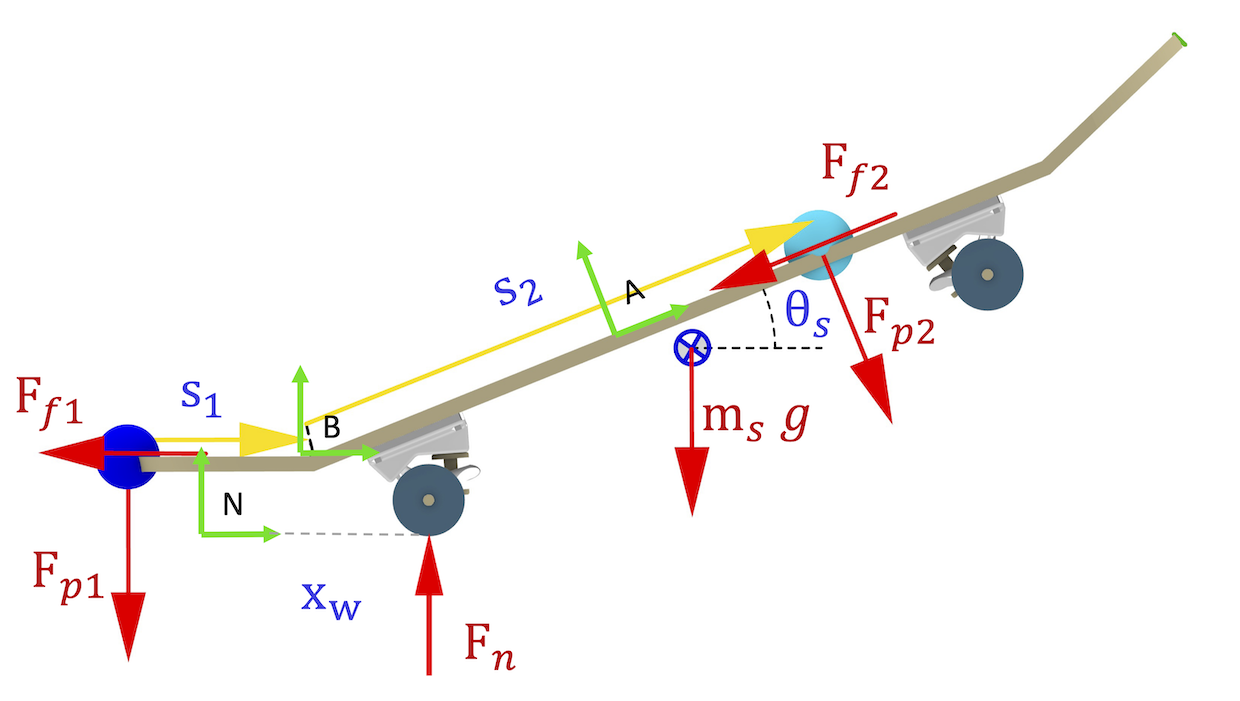
\includegraphics[width = 0.5\textwidth]{figure/FBD_phase1.png}
    \caption[Free body diagram phase 1]{Free body diagram phase 1. The back wheel is now modeled as sliding joint which reduces the degrees of freedom to 2. This is really  similar to the cart-pole problem. The equations are correct as long as the normal force at the wheel is not negative.}
    \label{f_FBDphas1}
\end{figure}
The EOM of the skateboard are derived with the TMT method \cite{vallery_heike_advanced_2018}. As stated in section \ref{s_phases}, the dynamics of phase 1 and 2 are different. The dynamics of phase 2 and 3 are the same. During phase 1 the EOM are derived with a sliding joint at the back wheel. This is done to eliminate the ground reaction forces from the EOM. The COM coordinates are

\begin{equation}
    \mathbf{x} = [x_s, y_s, \theta_s]^T
\end{equation}
The skateboard when considering the back wheel as a joint can be described by two generalized coordinates $x_w$ (x-location back wheels), and $\theta_s$ (angle w.r.t. ground) as shown in figure \ref{f_FBDphas1}. This is done to eliminate the ground reaction forces. The generalized coordinates are:
\begin{equation}
    \mathbf{q} = [x_w, \theta_s]^T
\end{equation}
And the CoM coordinates expressed in the generalized coordinates are:
\begin{equation}
\mathbf{x}=\left[\begin{array}{c}
\frac{l_{w b} \cos \left(\theta_s\right)}{2}+x_w+\left(d_{c o m}-h_{t r}\right) \sin \left(\theta_s\right) \\
\frac{l_{w b} \sin \left(\theta_s\right)}{2}+r_w+\left(h_{t r}-d_{c o m}\right) \cos \left(\theta_s\right) \\
\theta_s
\end{array}\right]
\end{equation}
Differentiating $\mathbf{x}$ once and taking the Jacobian with respect to the velocities gives transformation matrix T:
\begin{equation}
    J_{\dot{\mathbf{x}}}(\mathbf{q}) = \textbf{T} = \left[\begin{array}{c c}
1 & -\frac{l_{w b} \sin \left(\theta_s\right)}{2}+\left(d_{c o m}-h_{t r}\right) \cos \left(\theta_s\right) \\
0 & \frac{l_{w b} \cos \left(\theta_s\right)}{2}+\left(d_{c o m}-h_{t r}\right) \sin \left(\theta_s\right) \\
0 & 1
\end{array}\right]
\end{equation}
Convective terms $\mathbf{g_k}$ are found by taking the Jacobian of $\mathbf{\dot  x}$ with respect to $\mathbf{q}$ and multiplying it by $\mathbf{\dot  q}$ (e.g. $J_{\mathbf{\dot  x}}(\mathbf{q})\cdot \mathbf{\dot  q}$):

\begin{equation}
\mathbf{g_k} = 
\left[\begin{array}{c}
\dot \theta_s^2\left(-\frac{l_{w b} \cos \left(\theta_s\right)}{2}-\left(d_{c o m}-h_{t r}\right) \sin \left(\theta_s\right)\right) \\
\dot \theta_s^2\left(-\frac{l_{w b} \sin \left(\theta_s\right)}{2}+\left(d_{c o m}-h_{t r}\right) \cos \left(\theta_s\right)\right) \\
0
\end{array}\right]
\end{equation}
Two sets of bound vectors are equivalent when they equal resultants and equal moments about any point \cite{moore_force_nodate}. This means that all the forces acting on the skateboard can be described by resultant forces on and moments to the COM. The moments caused by the back and front foot about the COM are $Mc_{bf}, Mc_{ff}$ respectively. Thus the CoM-applied forces and torques $\mathbf{F_{a}}$ are:
 
\footnotesize
\begin{equation}\label{e_Fi}
\begin{array}{c}
    \mathbf{F_{a}}= \left[\begin{array}{c}
-F_{p 1} \sin \left(\phi-\theta_s\right)+F_{p 2} \sin \left(\theta_s\right)-F_{w 1} \cos \left(\phi-\theta_s\right)-F_{w 2} \cos \left(\theta_s\right) \\
-F_{p 1} \cos \left(\phi-\theta_s\right)-F_{p 2} \cos \left(\theta_s\right)+F_{w 1} \sin \left(\phi-\theta_s\right)-F_{w 2} \sin \left(\theta_s\right)-g m_s \\
Mc_{bf} + Mc_{ff}
\end{array}\right] 
\\ \\
Mc_{bf} = -F_{p 1} (-d_{\text {com }} \sin (\phi)-\frac{l_d \cos (\phi)}{2}-l_t+s_1)+F_{w 1}(d_{c o m} \cos (\phi)-\frac{l_d \sin (\phi)}{2})
\\ \\
\footnotesize Mc_{ff} = -F_{p 2}\left(-\frac{l_d}{2}+\mathrm{s}_2(t)\right)+F_{w 2} d_{c o m}
\end{array}
\end{equation}  
\smallskip
\normalsize
The skateboards' mass matrix $\mathbf{M_s} = diag(m_s,m_s,I_s)$ together with the transformed CoM applied coordinates form the EOM of phase 1:
\begin{equation} \label{e_eoma}
    \mathbf{T}^T \mathbf{M_s} \mathbf{T} \cdot \left[\begin{array}{c}
         \ddot x_w  \\
         \ddot \theta_s 
    \end{array}\right] = \mathbf{T}^T (\mathbf{F_a} - \mathbf{M_s} \cdot \mathbf{g_k})
\end{equation}
Rewriting the EoM gives two dynamical constraints valid for phase 1:
\begin{equation}
    \alpha_{3,4}^{(1)} =   \left(\mathbf{T}^T \mathbf{M_s} \mathbf{T} \cdot  \mathbf{T}^T\right)^{-1} (\mathbf{F_a} - \mathbf{M_s} \cdot \mathbf{g_k})
\end{equation}

\paragraph{Flight Equations of Motion - phases 2 and 3}
\noindent The EOM for phases 2 and 3 for the skateboard are without ground contact. The EOMs are derived similarly as the ground EOM, but now there generalized coordinates are the COM coordinates, since the body has 3 degrees of freedom. Thus $\mathbf{q} = \mathbf{x}$, which results in: $J_{\mathbf{\dot x}} \left(\mathbf{q}\right) = diag(1,1,1)$, and $\mathbf{g_k} = [0, 0, 0]^T$.  The COM applied forces $\mathbf{F_a}$ are the same as the ground EOM and don't need to be transformed. This gives the EOM of phases 2 and 3:
\begin{equation}\label{e_eomb}
\mathbf{M_s} \cdot \left[\begin{array}{c}
         \ddot x_s  \\
         \ddot y_s \\
         \ddot \theta_s 
    \end{array}\right] =  \mathbf{F_a}
\end{equation}
Which are in the same form as the Newton Euler equations (eq. \ref{e_newtoneuler}). This leads to the last two dynamic constraints valid for phase 2, and 3:
\begin{equation}
    \alpha_{5,6}^{(2,3)} = (\mathbf{M_s})^{-1}\mathbf{F_a}
\end{equation}
%%%%%%%%%%%%%%%% begin figure %%%%%%%%%%%%%%%%%%%
\begin{figure}[b]%
    \centering
    \subfloat[\centering 45.5" world record ollie. $^{1}$  ]{{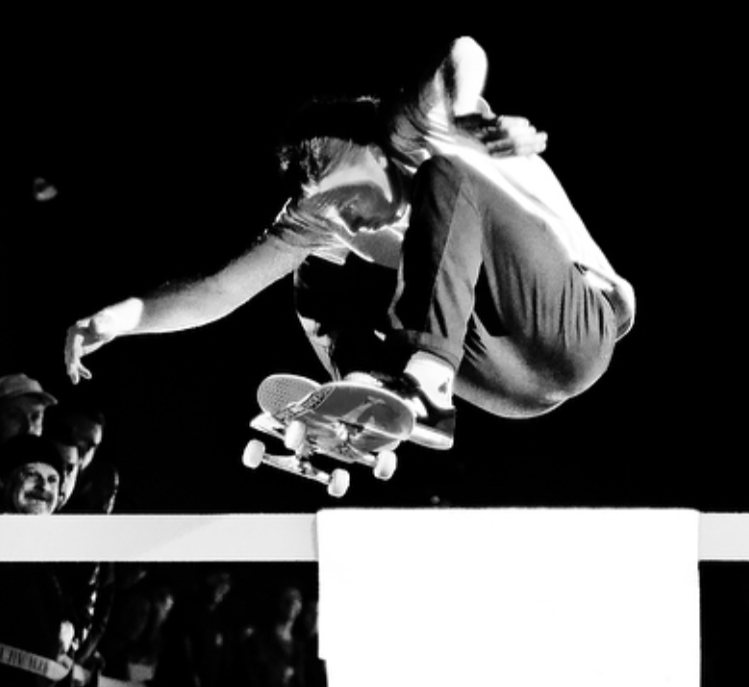
\includegraphics[width=0.2\textwidth]{figure/JakeHayes.png} }}%
    \quad
    \subfloat[\centering Yeadon model in same configuration]{{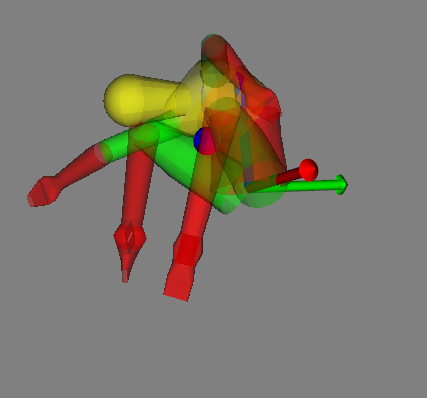
\includegraphics[width=0.2\textwidth]{figure/JakeHayesYeadon.png} }}%
    \caption{Reconstruction of world record ollie} 
    \label{fig:f_record}
    \centering \footnotesize \url{https://theberrics.com/world-record-ollie-footage}$^{1}$%
\end{figure}
%%%%%%%%%%%%%%%% end figure %%%%%%%%%%%%%%%%%%%
\subsubsection{Constraints}
\noindent Now that the dynamics are presented, we can move on to the constraints section. In this section the human kinetics and kinematics will be explained together with the friction model. 

\paragraph{Human}
\noindent The human is simplified as a point mass which reduces complexity for the optimization but sacrifices the reality. To make sure the human as a point mass still gives the output of a more complex model, the kinetics and kinematics will be constrained. 
\subparagraph{Kinematics}
\noindent The kinematics of the human controller are bound by the musculoskeletal restrictions of the human body. The musculoskeletal restricions are difficult to comprise in a point mass model. The first restriction is that the feet can only be within a certain distance of the human COM. This is not simply the leg length, because the COM location of the human will change when the legs are moved. The maximum and minimum feet location with respect to the COM of the human are found with Yeadon, a package for Python to configure a humanoid to a position and find distances between points \cite{yeadon_simulation_1990}. The model is set to a 1.80[m] tall human and is matched to a picture of the world record ollie of Jake Hayes. The reconstruction is seen in fig.\ref{fig:f_record}. The largest possible distance measured with the same model but now configured to an upright position. This leads to the first two constraint:


\begin{equation}\label{\e_yeadon}
\begin{split}
    \gamma_{1}^{(2,3)}:\quad  0.466 < y_h - \mathbf{r_{comH \mathbin{/} bf}} \cdot \mathbf{\hat n_y} < 1.13 \\ 
    \gamma_{2}^{(2,3)}:\quad  0.466 < y_h - \mathbf{r_{comH \mathbin{/} ff}} \cdot \mathbf{\hat n_y} < 1.13 
\end{split}
\end{equation}
These constraints describe that the vertical ($\mathbf{ \hat n_y}$) distance between the feet and the COM can never be outside of the given bounds. The constraint will become very complex if it would be the magnitude of the vector between the feet and the COM thus a vertical approximation is chosen. This constraint will not exceed musculoskeletal limits if the feet do not separate an an extreme distance (split). To make sure this behaviour does not happen, another constraint is implemented that the feet should never be separated more from each other than within a reasonable operating distance.
\begin{equation}
        \gamma_{3}^{(1,2,3)}:\quad   0.1 < |\mathbf{r_{bf/ff}}| < 1
\end{equation}
The skater should not leave the board in horizontal direction either. This gives the next constraint:
\begin{equation}
    \gamma_4^{(1,2,3)}:\quad  -0.3 < x_h - \mathbf{r_{comS\mathbin{/}comH}}\cdot \mathbf{\hat n_x} < 0.3
\end{equation}

To make sure the feet never leave the skateboard, $s_1$ and $s_2$ are positively bound from the end of the tail and the left pocket of the deck respectively (see fig \ref{f_FBD}. To make sure the feet do not leave the skateboard on the other end of the parts, two constraints are added:
\begin{equation}
\begin{array}{c}
    \gamma_{5}^{(1,2,3)}:\quad  0 < s_1-l_t < \infty  \\
    \gamma_{6}^{(1,2,3)}:\quad  0 < s_2-l_d < \infty  \\
\end{array}
\end{equation}
The feet can still be in a no contact scenario as seen in section \ref{ss_mechanics}. This is simulated by when zero force is exerted. 

\subparagraph{Kinetics}
\noindent The kinetics of the human are bound to the characteristics of the countermovement jump (CMJ) during the first phase of the ollie. The CMJ motion is chosen because, 76.3\% of the variance in the performance of the ollie maneuver can be explained by the CMJ (CMJ) \cite{candotti_lower_2012}. The CMJ is reported to have good reliability and is a strong assessment of lower-body mechanical power \cite{barker_relationships_2018}. During a vertical jump, joint torques, knee extensor force, hip abduction forces all map to one output variable: the ground reaction force. The only sensible way to capture the kinetics of a human jumper for a point mass model is the ground reaction force, because only more complex approximation can capture contributions of individual segments. Thus, the ground reaction force of the CMJ is used to realize a realistic COM human jumper model. In figure \ref{f_cmj} a typical ground reaction force for a CMJ is shown. By constraining the vertical rate of force development (RFD) ($dF/dt$, slope in figure \ref{f_cmj}), the maximum force $F_{max}$, maximum displacement $\Delta s$, and maximum mechanical power $P$, the total mechanical output of the legs is constrained for a simple point mass model. By constraining the RFD, the shortening or lengthening cycle is simulated. The maximum force will make sure the force does not exceed the maximum capabilities. By constraining the power, given a constrained force, the maximum velocity is also constrained due to $P = F v_{rel}$.
Due to a constrained maximum distance($\Delta s$) the force can work over, the work done is also constrained due to $W = F ds$, given a constrained force. The data for the RFD, $F_{max}$, $\Delta s$, $P$ is taken from a Division-I male, soccer players with a mean height of 179.5[cm], weight of 75.5[kg], and age of 19.65 years \cite{barker_relationships_2018}. $\Delta s$ and $P$ are calculated in the paper with a point mass approximation which is important to map to the optimization properly. The data was measured for two legs simultaneously, which is unfortunate for the optimization since the two legs can work separately and which might lead to different kinetic data. Though, the constraints are set on the sum of the forces and the forces separately due to the possibility of out of phase pushing and pulling which could result in a combined satisfaction of the constraint but individual legs could exceed the physical limitations. The maximum distance is constraint implemented similar to equation \ref{\e_yeadon} with the same upper bound:
\vspace{-0.1in}
\begin{equation}
\begin{split}
        \gamma_{7}^{(2,3)}:& \quad  1.13-\Delta s < y_h - \mathbf{r_{comH \mathbin{/} bf}} \cdot \mathbf{\hat n_y} < 1.13 \\ 
      \gamma_{8}^{(2,3)}:& \quad  1.13-\Delta s < y_h - \mathbf{r_{comH \mathbin{/} ff}} \cdot \mathbf{\hat n_y} < 1.13 
      \end{split}
\end{equation}

\begin{figure}
    \centering
    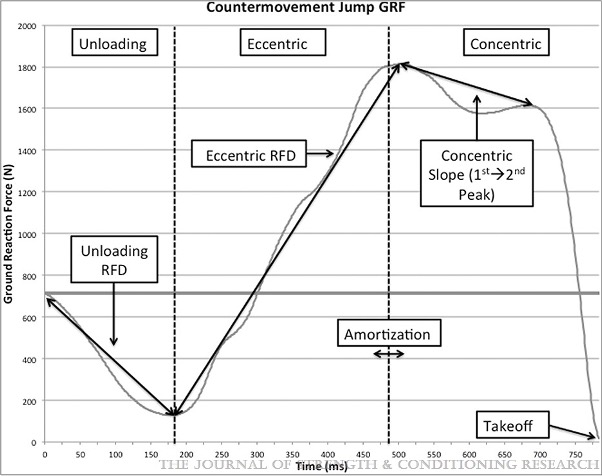
\includegraphics[width=0.4\textwidth]{figure/countermovementjumpRFD.jpg}
    \caption[Ground reaction force of CMJ]{Phases during CMJ. During unloading, the human lowers their COM quickly. During the eccentric phase, the gained downward velocity during the unloading phase is braked until the lowest point is reached which is at the amortization. During the concentric phase the legs are stretched out and upward speed is gained until the take-off. At take-off the vertical speed is maximal.}
    \centering \footnotesize Source: \cite{barker_relationships_2018}%
    \label{f_cmj}
\end{figure}
\noindent The maximum force constraints are set at the sum of all vertical forces $\mathbf{F_h}\cdot \mathbf{\hat n_y}$, and to the vertical components of the back and front feet ($\mathbf{F_{bf}}\cdot \mathbf{\hat n_y}, \mathbf{F_{ff}}\cdot \mathbf{\hat n_y}$)
\begin{equation}
\begin{array}{c}
    \gamma_{9}^{(1,2,3)}:\quad  -32.61 m_h < \mathbf{F_h}\cdot \mathbf{\hat n_y} < 32.61 m_h   \\
    \gamma_{10}^{(1,2,3)}:\quad  -32.61 m_h < \mathbf{F_{bf}}\cdot \mathbf{\hat n_y} < 32.61 m_h \\
    \gamma_{11}^{(1,2,3)}:\quad  -32.61 m_h < \mathbf{F_{ff}}\cdot \mathbf{\hat n_y} < 32.61 m_h \\
\end{array}
\end{equation}
The unloading RFD ($-41.8 m_h$) and eccentric RFD ($196.41 m_h$) are implemented in the constraints:
\begin{equation}
    \begin{array}{c}
        \gamma_{12}^{(1)}:\quad  -41.8 m_h < \dot \mathbf{F_h}\cdot \mathbf{\hat n_y} < 196.41 m_h   \\
    \end{array}
\end{equation}
The power is found per leg by calculating the dot product between relative velocity between the foot and the human COM and the resultant force acting on the foot. 
\begin{equation}\label{e_power}
    \begin{array}{c}
         P_{bf} = \mathbf{\dot r}_{comH/bf} \cdot \mathbf{F_bf}  \\
         P_{ff} = \mathbf{\dot r}_{comH/ff} \cdot \mathbf{F_bf}  \\
    \end{array}
\end{equation}
Just like the maximum force constraints, the legs can work out of phase (one leg negative work, one leg positive). To avoid that the limits are exceeded the power needs to be bound absolutely. Absolute values are not feasible in higher order optimization problems like this one \cite{kelly_introduction_2017}. Though a trick like these constraints can create an absolute bound in the constraint space, resulting in the following constraints:
\begin{equation}
    \begin{array}{c}
         \gamma_{13}^{(1)}:\quad  -54.62 m_h < P_{bf} + P_{ff} < 54.62 m_h  \\
         \gamma_{14}^{(1)}:\quad  -54.62 m_h < P_{bf} - P_{ff} < 54.62 m_h  \\
         \gamma_{15}^{(1)}:\quad  -54.62 m_h < P_{ff} - P_{bf} < 54.62 m_h  \\
    \end{array}
\end{equation}
The horizontal ($\mathbf{\hat n_x}$) direction forces are now unconstrained. The data in from the CMJ paper does not include any horizontal forces. Since the body of the human does not rotate during the jump, the horizontal forces are approximated with maximum abduction force. The maximum abduction force is obtained by pushing sideways against a scale whilst standing up-straight. This maximum force bound is not very accurate, but the power of abduction force is captured in the power calculation in equation \ref{e_power}. This leads to a reliable abduction force approximation. With the constraints:
\begin{equation}
    \begin{array}{c}
         \gamma_{16}^{(1,2,3)}:\quad  -200 < \mathbf{F_{ff}}\cdot \mathbf{\hat n_x} < 200  \\
         \gamma_{17}^{(1,2,3)}: \quad -200 < \mathbf{F_{ff}}\cdot \mathbf{\hat n_x} < 200 \\ 
    \end{array}
\end{equation}
Only the maximum force constraints $\gamma_{11-13}$ and $\gamma_{18-19}$ apply to all phases. The CMJ constraints are only applied to the first phase, since phase 1 concerns the CMJ movement. 

\paragraph{Friction}
\noindent According to section \ref{ss_mechanics} the feet are sliding along the griptape to level the skateboard out and drag the skateboard up during the preparation phase 1, and upward motion phase 2. The used method implements static and dynamic friction and is a simplification to the frictional contact implicit optimization called the relaxed formulation by Patel et al. \cite{patel_contact-implicit_2019}. This method is able to have unplanned discontinuous frictional contact with direct collocation without a hybrid method. Usually this would be considered impossible since direct collocation enforces the dynamics and constraints over a continuous domain, where discontinuities in the system dynamics usually lead to infeasibility \cite{kelly_transcription_2017}. The downside is that with this method it is difficult to converge to a feasible solution without a proper initial guess and the computation time is rather high \cite{shield_contact-implicit_2022,patel_contact-implicit_2019}. I have found a way to simplify this method, which represents a contact implicit frictional contact that solves optimally under 2 minutes without initial guess. To explain the simplifications and for the sake of clarity, I will first explain the impact method of Patel et al., but I won't use this in my optimization.

%%%%%%%%%%%%%%%% begin figure %%%%%%%%%%%%%%%%%%%
\begin{figure}
\centerline{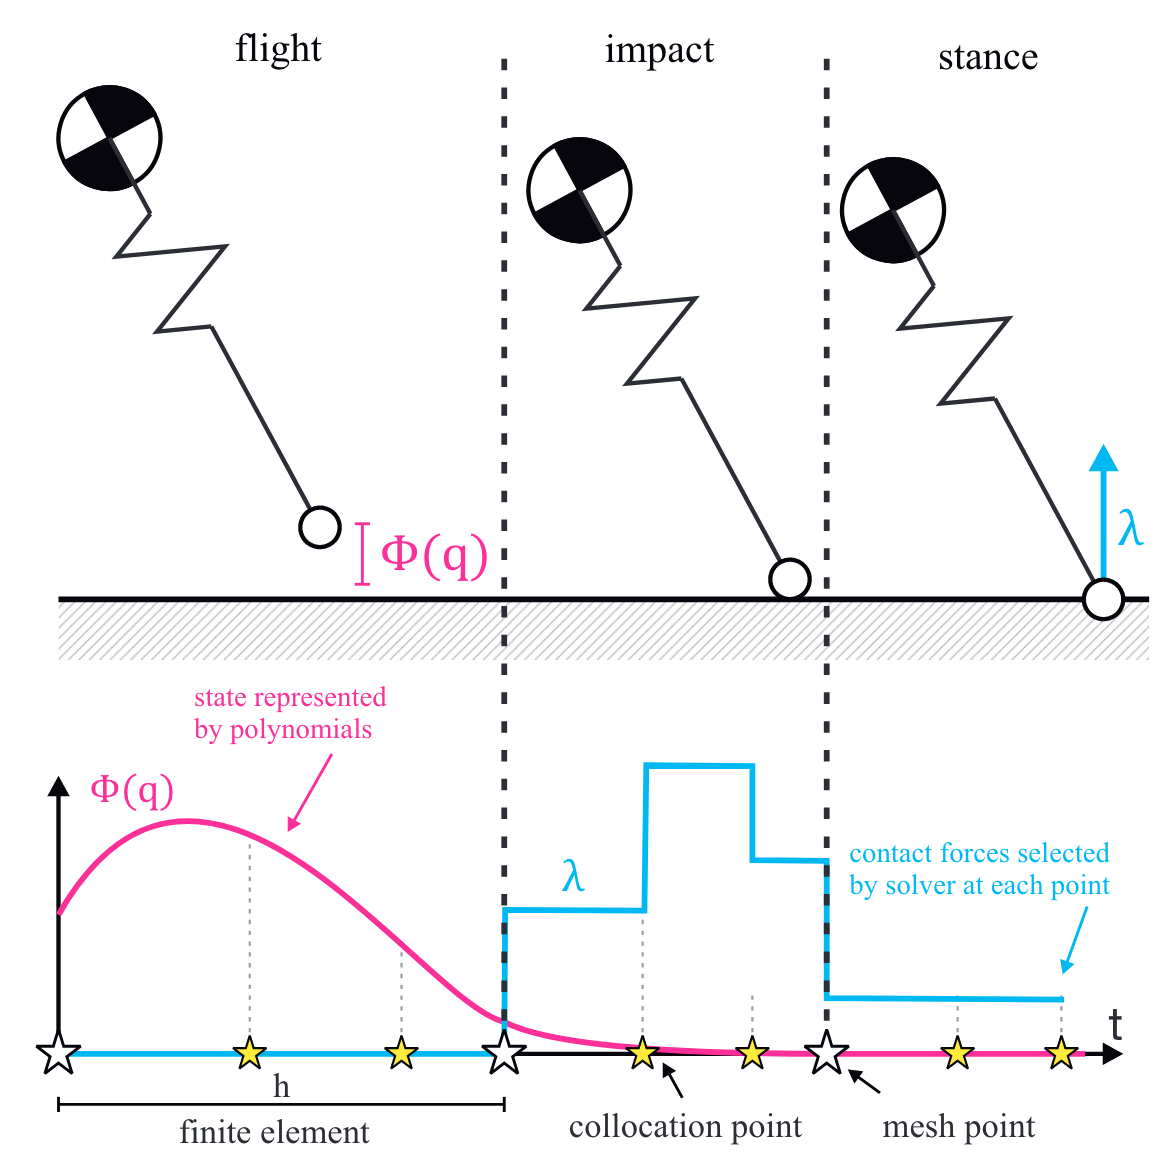
\includegraphics[width=0.4\textwidth]{figure/relaxed_method.png}}
\caption[Relaxed impact method]{Relaxed impact formulation. Contact mode is changed at each mesh point, the contact force $\lambda$ is selected by solver at each collocation point. Source: \cite{patel_contact-implicit_2019}}
\label{f_relaxed}
\end{figure}
%%%%%%%%%%%%%%%% end figure %%%%%%%%%%%%%%%%%%%

The relaxed formulation is shown in figure \ref{f_relaxed}. It implements a contact constraint that will look one time-step ahead to be able to initiate a contact force before impact. Let $C_c(\mathbf{q})$ be the relative distance between the two bodies that impact, and let the normal force $F_n$ be a control variable. The following constraints will ensure that only when the next time step is in contact ($C_c(\mathbf{q}(t+1)$) the normal force $F_n > 0$ when there is no contact at the next time step, $F_n$ must be zero:
\begin{equation}\label{e_patelimpact}
    F_n\ C_c(\mathbf{q}(t+1) = 0,\quad C_c(\mathbf{q}) \geq 0,\quad F_n \geq 0
\end{equation}
This result of this formulation is shown graphically in figure \ref{f_discontinuities}. When constraining an optimization problem likewise, the solver will find the normal forces needed to comply to the non penetration constraint $C_c(\mathbf{q}) \geq 0$. This method has been used in the optimization of an ollie. Though the initial guess needed to be similar to the solution to find feasible solutions. The model with a full body human operator took 43 minutes to solve \cite{shield_contact-implicit_2022}. 
To simplify the model I excluded this impact formulation, because I assume that the feet are always located on the skateboard, but can be out of contact by exerting zero force. In this case, where the human is not modeled with multiple segments but as a point mass, it is possible to exclude equation \ref{e_patelimpact}. By setting the normal forces of the feet $F_{p1},F_{p2}$ as control variables. The foot location is also regulated by a control variables. The acceleration is controlled instead of the foot location itself to still have smooth realistic foot trajectories. Resulting in the control variables:
\begin{equation}
    \mathbf{u}^{(1,2,3)} = [F_{p1},F_{p2},\ddot s_1, \ddot s_2]    
\end{equation}

Now that the difficult to solve contact formulation by Patel in equation \ref{e_patelimpact} is replaced by a simplified formulation, I will continue with the friction model that is used in this optimization.
Friction is present during the ollie when sliding the foot along grip-tape, when rolling, and when the tail hits the ground if the tail has a relative velocity tangential to the impact surface. Friction is a highly non-linear and discontinuous phenomenon. In general the dominant friction components that have been modeled include static friction (A force that opposes the input force at zero velocity), Coulomb friction (constant motion opposing force at non-zero velocity), viscous friction (when fluid exists between the contact surfaces), and the Stribeck effect (a speed dependent friction) \cite{makkar_new_2005}. 
\begin{figure}
    \centering
    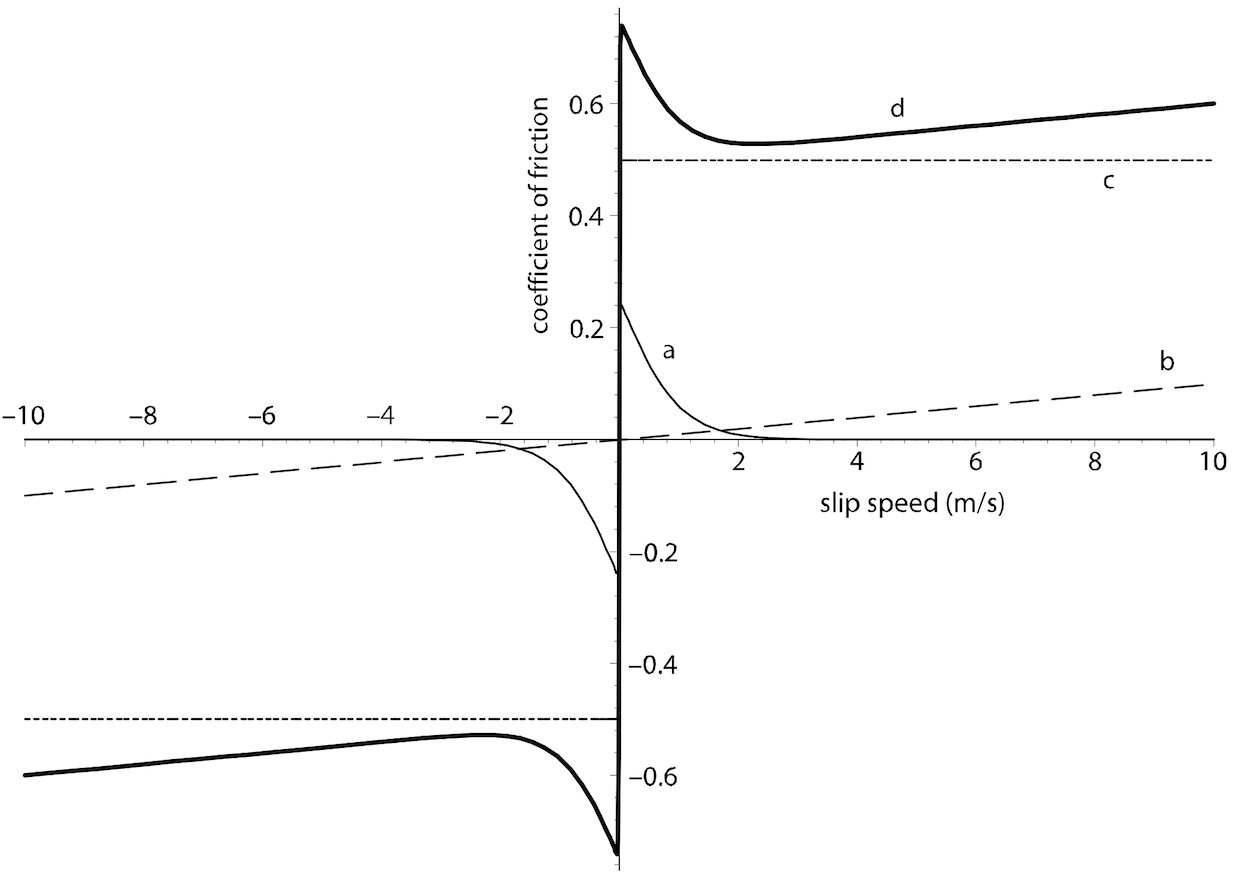
\includegraphics[width=0.4\textwidth]{figure/friction_.png}
    \caption[Friction effects]{Friction model as a composition of different effects including a) Stribeck effect, b) viscous dissipation, c) coulomb effect, d) combined model}
    \label{f_friction}
\end{figure}

%When modeling friction continuously, pure static friction does not exist since at zero velocity the friction function will be zero as well due to symmetry. 
Just like the normal force, friction can also only exist during contact. The friction is solved with a set of constraints. The first step to implement this friction is to create slack variables that divide the friction forces as described in the system dynamics $F_{f1},F_{f2}$ into a positive and negative components. For simplicity reasons I will only derive the friction of the back foot along the skateboard. The front foot friction is obtained by exactly the same process. By replacing $_1$ to $_2$ in the following equations, the front foot friction is also realized
\begin{equation} \label{e_plusminfric}
   F_{f1} = F_{f1}^+ - F_{f1}^- 
\end{equation}
As described in section \ref{s_systemdynamics}, the forces perpendicular to the skateboard are positive definite such that the force can never pull on the skateboard. Now the created slack variables also need to be positive definite:
\begin{equation}
    F_{p1} \geq 0,\quad F_{f1}^+ \geq 0,\quad F_{f1}^- \geq 0  
\end{equation}
Static and dynamic friction is bound by the friction cone shown in figure \ref{f_frictioncone}. The magnitude of dynamic friction is $F_{p1}\ \mu$ with a direction opposed to the relative sliding velocity (see figure \ref{f_frictioncone}. The static friction is bound by the whole surface of the friction cone and is only possible when the feet are not sliding. To realize this, another slack variable $\psi$ is introduced which represents the magnitude of the relative velocity $\dot s_1$ between the foot and the skateboard. 
\begin{equation}
\begin{split}
    \gamma_{18}^{(1,2,3)}: \quad & \psi_1 + \dot s_1  \geq 0 \\
    \gamma_{19}^{(1,2,3)}: \quad & \psi_1 - \dot s_1  \geq 0 \\
\end{split}
\end{equation}
Now static friction can be implemented with a set of constraints:
\begin{equation}
\begin{split}\label{e_frictioncontrol}
       \gamma_{20}^{(1,2,3)}: \quad & \mu F_{p1} - F_{f1}^+ - F_{f1}^- \geq 0 \\
       \gamma_{21}^{(1,2,3)}: \quad & (\mu F_{p1} - F_{f1}^+ - F_{f1}^-)\ \psi_1  = 0
\end{split}
\end{equation}
The first constraint assures that the positive component or the negative component of the friction is always smaller than $\mu F_{p1}$. The second constraint makes sure that when the foot slides ($\psi_1 \not = 0$),  the sum of the positive and negative friction components equal $\mu F_{p1}$. It is important that when sliding in positive direction, the negative friction component $F_{f1}^-$ should equal $\mu F_{p1}$ and $F_{f1}^+=0$ and vice versa. This is realized with the following constraints:
\begin{equation}
\begin{split}
    \gamma_{22}^{(1,2,3)}: \quad & F_{f1}^+ (\psi_1 + \dot s_1)  = 0 \\
    \gamma_{23}^{(1,2,3)}: \quad & F_{f1}^- (\psi_1 - \dot s_1)  = 0
\end{split}
\end{equation}
This type of constraint ($A\cdot B = 0$) has three possible solutions $A= 0,\ B=0,\ or\ A,B = 0$. By filling in a numerical example, the desired behaviour is shown. For example looking at the first constraint, when $\dot s_1 = -1$, then $\psi_1 + \dot s =  0$ and $F_{f1}^+$ can be a positive number. Then looking at the second constraint, when $\dot s = -1$, then $\psi - \dot s = 2$ and $F_{f1}^- = 0$. Combining this with the second equation in equation \ref{e_frictioncontrol} gives: $(\mu F_{p1} - F_{f1}^+ - 0) \cdot 0 = 0$, which results in $F_{f1}^+ = \mu F_{p1}$. This is exactly what it should be given a negative relative sliding velocity. 
The friction for the front foot will be another six constraints: $\gamma_{24-30}^{(1,2,3)}$ 
\begin{figure}
    \centering
    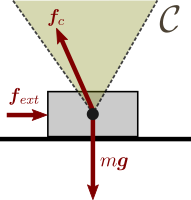
\includegraphics{figure/Frictioncone.png}
    \caption[friction cone]{$f_c$ is the reaction force exerted by the ground on the box, which is composed of a normal force $f_n$ equal and opposite to $mg$ and friction $f_w$ equal and opposite to $f_{ext}$. The box is stationary if $f_{ext} < f_n\ \mu$. Static friction is bound by $-f_n\ \mu < f_w < f_n\ \mu$. But when $f_{ext}\ >\ f_n\ \mu$, the box will start to slide with velocity $v$ and $f_w = f_n\ \mu$. Dynamic friction is described by $f_w = -sign(v) f_n\ \mu$. The top of the cone is unbound, because when a vertical external load would be applied, the normal force would change in magnitude.} 
    \footnotesize Source:\url{https://scaron.info/robot-locomotion/}
    \label{f_frictioncone}
\end{figure}

\subsubsection{Endpoint constraints} \label{p_endpoints}
\noindent To fully describe the ollie optimization problem, all phases need to be glued together. In the multi-phase optimization scheme all initial and final time variables are treated as separate variables. By constraining the corresponding variables between the phases, the variables can be treated as one variable over all three phases.

\paragraph{Impact}
\noindent Just before the skateboard is airborne, the tail hits the ground. During this collision the ground exerts a linear impulse normal to the ground. The method by Vallery and Schwab \cite{vallery_heike_advanced_2018} is based on the Newton impact law. The Newton impact law rewritten in terms of the optimization states is:
\begin{equation}\label{e_newtonimpact}
    \mathbf{\dot q_{rel}}^{(2)}(t_0) = -e\ \mathbf{\dot q_{rel}}^{(1)}(t_F)
\end{equation}
Where $\dot q_{rel}^{(2)}(t_0)$, and $\dot q_{rel}^{(1)}(t_F)$ are the relative speeds just after impact at the first collocation point of phase 2, and just before impact at the last collocation point of phase 1 respectively.  $e$, the empirical constant related to the amount of dissipated energy during impact, is called the coefficient of restitution (COR). When $e=1$ we have mechanical energy preservation, and for $e=0$ all impact energy is lost into dissipation. Now lets write this equation in matrix form. Let $C_c(\mathbf{q})$ be the relative distance normal to the contact surface. By taking the Jacobian with respect to the generalized coordinates and multiplying it with the generalized velocities we find the relative generalized velocity:
\begin{equation}\label{e_relativevelocity}
    \frac{d}{dt}\left(C_c(\mathbf{q})\right) = J_{\mathbf{q}}(C_c(\mathbf{q}))\ \mathbf{\dot q} = \mathbf{C_{c,i}}\  \mathbf{\dot q}
\end{equation}
Combine equations \ref{e_newtonimpact}, and \ref{e_relativevelocity} to get:
\begin{equation}
    \mathbf{C_{c,i}}\  \mathbf{\dot q}^{(2)}(t_0) = -e\ \mathbf{C_{c,i}}\ \mathbf{\dot q}^{(1)}(t_F)
\end{equation}
Now by introducing a Langrange multiplier $\rho_c$ which is used to solve the reaction impulse calculated with $\mathbf{C_{c,i}}\ \rho_c$ the linear impulse and momentum equation is:
\begin{equation}\label{e_linearimpulse}
    \mathbf{M_s}\ \mathbf{\dot q}^{(2)}(t_0) + \mathbf{C_{c,i}}\ \rho_c = \mathbf{M_s}\ \mathbf{\dot q}^{(1)}(t_F)
\end{equation}
Where $\mathbf{M_s}$ is the mass matrix of the system. Now writing equation \ref{e_linearimpulse} with equation \ref{e_relativevelocity} as an added constraint the velocities after impact are solved. This gives the first four endpoint constraints that define the impact of the tail:
\begin{equation}
    \beta_{1,2,3,4}: \quad \left[\begin{array}{cc}
        \mathbf{M_s} & \mathbf{C_{c,i}} \\
        \mathbf{C_{c,i}}^T & 0
    \end{array} \right]\
    \left[\begin{array}{c}
       \mathbf{\dot q}^{(2)}(t_0)  \\
        \rho_c 
    \end{array}\right] = 
    \left[\begin{array}{c}
         \mathbf{M_s}\ \mathbf{\dot q}^{(1)}(t_F)   \\
         -e\ \mathbf{C_{c,i}}^T\ \mathbf{\dot q}^{(1)}(t_F)
    \end{array}\right]
\end{equation}

Because the states in phase 1 are expressed in different variables than phase 2 as shown in section \ref{s_systemdynamics}, variables $\dot q^{(1)}(t_F)$ needs to be rewritten to the CoM coordinates $x_s,y_s$, and $\theta_s$. Also the initial values of variables $x_s^{(2)}(t_0), y_s^{(2)}(t_0)$ are dependant on the final time variables $x_w^{(1)}(t_F), \theta_s^{(1)}(t_F)$ and are set as an endpoint constraint
\footnotesize
\begin{equation}
\begin{split}
\beta_5:& \ x_s^{(2)}(t_0) = \frac{l_{w b} \cos \left(\theta_s\right)}{2}+x_w^{(1)}(t_F)-\left(-d_{c o m}+h_{t r}\right) \sin \left(\theta_s^{(1)}(t_F)\right) \\
\beta_6:& y_s^{(2)}(t_0) = \frac{l_{w b} \sin \left(\theta_s\right)}{2}+r_w+\left(-d_{c o m}+h_{t r}\right) \cos \left(\theta_s^{(1)}(t_F)\right)
\end{split}
\end{equation}
\normalsize
%%%%%%%%%%%%%%%% begin figure %%%%%%%%%%%%%%%%%%%
\begin{figure}
\centerline{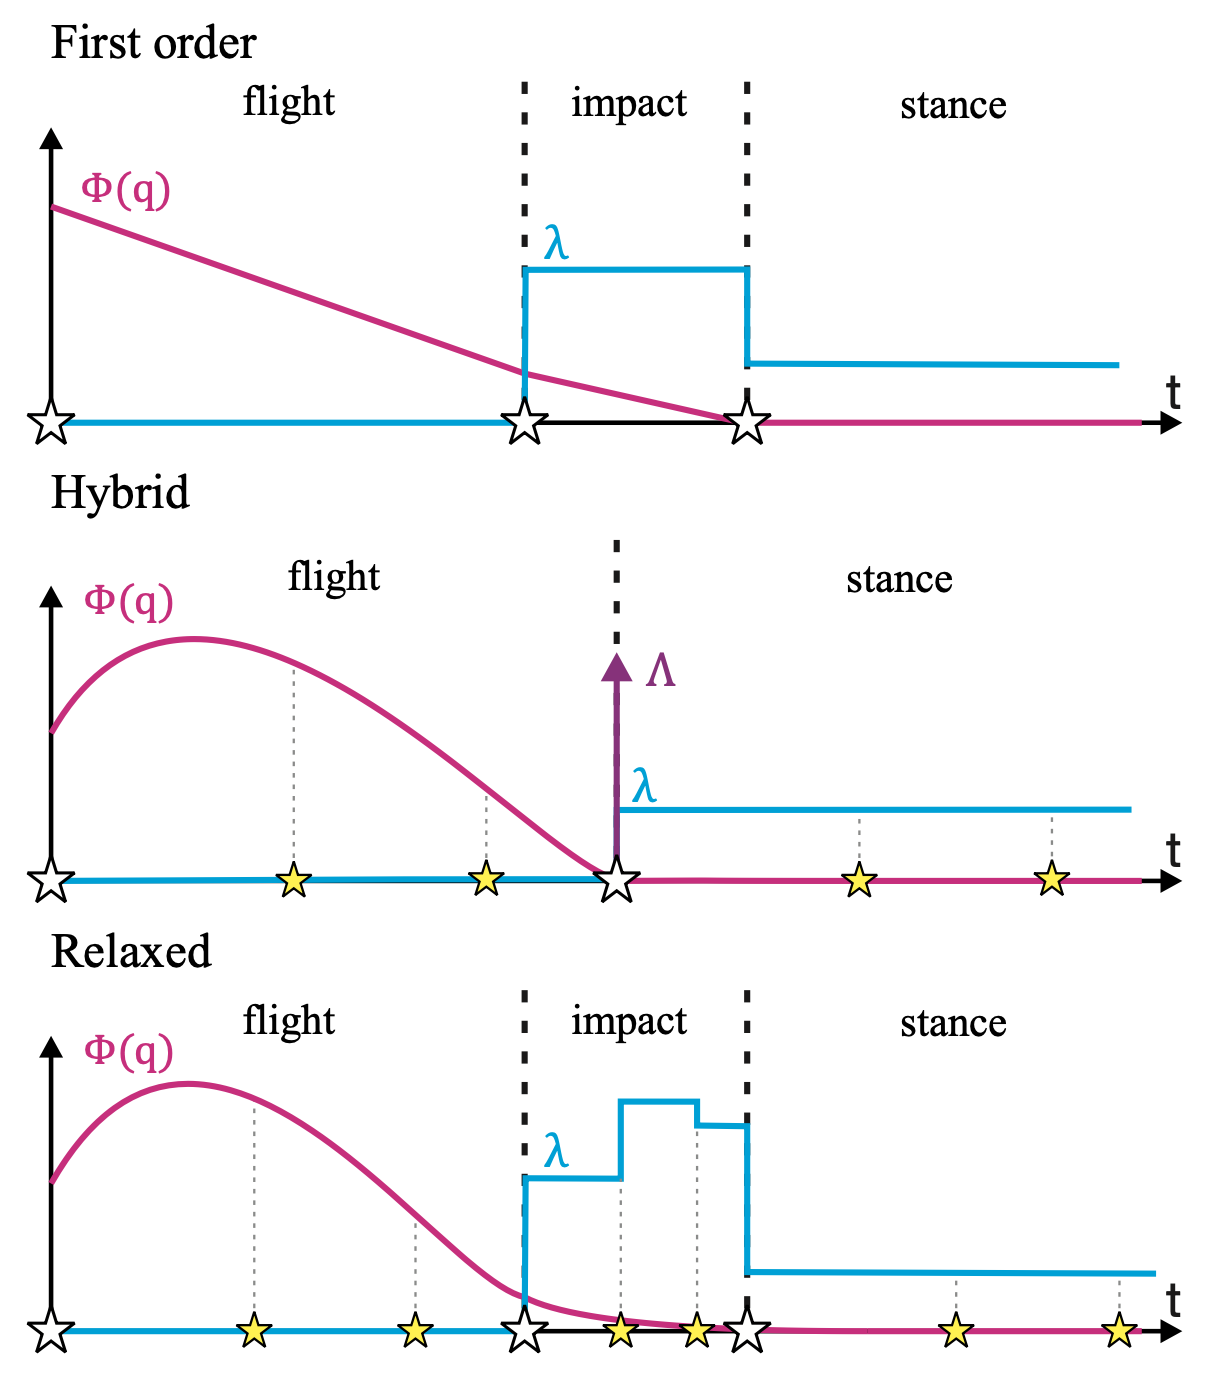
\includegraphics[width=0.3\textwidth]{figure/impactmethods.png}}
\caption{Three impact models used in optimization \cite{patel_contact-implicit_2019}. }
\label{f_discontinuities}
\end{figure}
%%%%%%%%%%%%%%%% end figure %%%%%%%%%%%%%%%%%%%

This method is a discontinuous method where velocity states will have jumps as seen in figure \ref{f_discontinuities}, second graph. This is opposed to continuous methods that will continuously change the velocity state over time (figure \ref{f_discontinuities} first graph). For example Ackerman and van den Bogert \cite{ackermann_optimality_2010} modeled the ground as a spring damper system that exerts a force when the contact point penetrates the contact surface with a gait optimization. When spring damper constants are implemented correctly, the energy should be dissipated during contact. The advantages of this model is that in an optimization the states are all continuous. This makes it possible to have unplanned impact (contact implicit optimization). In other words, you are not prescribing when and how impact occurs. The disadvantage of this model is that it is rather unaccountable for the actual force output. When solving such a problem imagine that an object is about to encounter impact and penetration depth equals 0, the states have a velocity state $v$ towards to the contact surface. The penetration depth of the next time step with a simple forward Euler integration will be $v \delta t$. This means that the magnitude of the time step will influence the penetration depth, which in terms influences the force output. The used discontinuous method will be independent of time step size and the ground does not have to be modeled complexly to get a desired force output. Furthermore, the behaviour of the impact will be constant over different iterations with different solutions, and will be more precise since a higher order optimization method can be used. 

\paragraph{Time}
\noindent The result of the optimization should be continuous in time over all three phases. This is obtained by endpoint constraints: 
\begin{equation}
    \begin{array}{c}
         \beta_7: \quad t_F^{(1)} = t_0^{(2)}  \\
         \beta_8: \quad t_F^{(2)} = t_0^{(3)}  \\
    \end{array}
\end{equation}

The time variables are set as optimization variables, meaning that the optimization should know when to switch phase. This is done by the impact angle of the skateboard. This is a function of the parameter values:
\begin{equation}
    \theta_{impact} = -\operatorname{atan}\left(\frac{h_{t r}+l_t \sin (\phi)+r_w}{-\frac{l_d}{2}-l_t \cos (\phi)+\frac{l_{w b}}{2}}\right)
\end{equation}
The end of phase 1 should equal this angle. This is obtained with endpoint constraints:
\begin{equation}
    \beta_7: \quad \theta_s^{1}(t_F) = \theta_{impact}
\end{equation}

To make sure the human starts the ollie from a standing position, the vertical forces at the beginning of phase 1 are equal to the bodyweight:
\begin{equation}
    \beta_8: \quad \mathbf{F_h} \cdot \mathbf{\hat n_y} = m_h g
\end{equation}

The definition of landing the ollie has been set to the back wheel touching the ground at a minimum of 0 [rad] (level) and a maximum of $\frac{1}{6} \pi$[rad] (rotated counter clockwise sligthly). The optimization stops when the backwheel touches the ground.

\begin{equation}
    \beta_9 : \frac{-l_{wb}}{2} \sin(\theta_s(t_F^{(2)})) - r_w + y_s(t_F^{(2)}) + (d_{com} - {d_tr}) \cos(\theta_s(t_F^{(2)}))
\end{equation}
Variables $\theta_s, s_1, s_2, \dot s_1, \dot s_2, x_h, y_h, \dot x_h, \dot y_h$ have equal endpoints between phase 1 and 2 ($b_{9-18})$. All state variables have equal endpoints between phase 2 and 3 ($b_{18-32}$). Initial and final endpoint constraints are set to a wide range and are found in Appendix B, \ref{t_constraints}.

\subsection{Settings}\label{s_settings}
\noindent The NLP tolerance is set to $1e^{-8}$, and the mesh tolerance is set to $1e^{-3}$. The amount of mesh sections for the first two phases are set to 30, phase 3 is set to 10 mesh sections. The landing phase is not as important as the preparation and upward motion phase as those define the final height and thus the objective.


\subsection{Summary}\label{s_summary}
\noindent To summarize all the findings, the general formula for the multi-phase ollie OCP is implemented in one overview. The objective function for the ollie OCP is 
\begin{equation}
     maximize\ (y_s^{(2)}(t_F) + d_{com} - h_{tr} - r_w)
\end{equation} 
Subject to the dynamical constraints in phase 1:
\begin{equation}
\begin{array}{c}
        \alpha_{1} = \frac{\mathbf{F_h}\cdot \mathbf{\hat n_x}}{m_h}\\
        \alpha_{2} = \frac{\mathbf{F_h}\cdot \mathbf{\hat n_y}}{m_h}\\
        \alpha_{3,4}^{(1)} =   \left(\mathbf{T}^T \mathbf{M_s} \mathbf{T} \cdot  \mathbf{T}^T\right)^{-1} (\mathbf{F_a} - \mathbf{M_s} \cdot \mathbf{g_k})
\end{array}
\end{equation}
And for phase 2 and 3:
\begin{equation}
    \begin{array}{c}
        \alpha_{1} = \frac{\mathbf{F_h}\cdot \mathbf{\hat n_x}}{m_h}\\
        \alpha_{2} = \frac{\mathbf{F_h}\cdot \mathbf{\hat n_y}}{m_h}\\ 
        \alpha_{5,6} = (\mathbf{M_s})^{-1}\mathbf{F_a}
    \end{array}
\end{equation}
With path constraints during phase 1:
\begin{equation}
    \begin{array}{c}
         \gamma_{3-6},  \\
         \gamma_{9-30},
    \end{array}
\end{equation}
And during phase 2 and 3:
\begin{equation}
    \begin{array}{c}
         \gamma_{1-11}  \\
         \gamma_{16-30}
    \end{array}
\end{equation}
With endpoint constraints $\beta_{1-9}$.
In the first phase the state variables $q^{(1)}$, control variables $u_c^{(1)}$, slack control variables $u_s^{(1)}$ are:
\begin{equation}
\begin{array}{rl}
   \mathbf{q^{(1)}} =& [x_w , th_s, x_h, y_h, \dot x_w, \dot th_s,\dot x_h, \dot y_h]    \\
   \mathbf{u_c^{(1)}} =& [fp1, fp2, dds_1, dds_2]  \\
   \mathbf{u_s^{(1)}}=&  [F_{f1}^+, F_{f1}^-, \psi_1,F_{f2}^+, F_{f2}^-, \psi_2] 
\end{array}
\end{equation}
During the second and third phase the state variables $q^{(2,3)}$, control variables $u_c^{(2,3)}$, slack control variables $u_s^{(2,3)}$ are:
\begin{equation}
\begin{array}{rl}
   \mathbf{q^{(2,3)}} =& [x_s, y_s, \theta_s, x_h, y_h, \dot x_s, \dot y_s, \dot \theta_s,\dot x_h, \dot y_h]    \\
   \mathbf{u_c^{(2,3)}} =& [F_{p1}, F_{p2}, \ddot s_1, \ddot s_2]  \\
   \mathbf{u_s^{(2,3)}}=&  [F_{f1}^+, F_{f1}^-, \psi_1,F_{f2}^+, F_{f2}^-, \psi_2] 
\end{array}
\end{equation}
With the global parameters variables $\sigma$ as any combination of the optimized geometric parameters: 
\begin{equation}
    \sigma_i \in [l_{wb}, l_d, l_t, \phi, h_{tr}, r_w]
\end{equation}

The results will show several optimizations with different combinations of parameter optimizations to search the solution space for optimal shapes. The first set of optimizations will be without optimized parameter variables to show proper functioning of the model. The second set of optimizations will be single variable optimizations where only one variable from the optimized parameter variables is chosen to be optimized. The third set of optimization will be variations to multiple optimized parameter variables. The results will show the optimal trajectories and geometries of these optimizations together with detailed trajectories over time a video posted on youtube created by the model.



\section{Results}
\noindent Figures \ref{f_singlepar}, and \ref{f_multipar} show 9 skateboard shapes that have improved ollie height compared to the industrial standard Popsicle stick skateboard geometry (Base in figure \ref{f_nopar}) when optimized for optimal ollie height. The best performing skateboard shape (number 2 in figure \ref{f_multipar} improved ollie height by 11.1 \%. All optimizations are with a null seed initial guess and solved with an optimal IPOPT exit status with the desired NLP tolerance and mesh tolerance found in \ref{s_settings}. All optimizations were solved within 3 minutes. Four skateboards did not show improvement in ollie height, which are indicated with a red dot. These are per definition local maxima, because the base optimization is a higher solution, which is in the solution space of these optimizations. 

\subsection{Optimal Trajectories and \\Geometries}
\subsubsection{No parameter optimization}
\begin{figure*}
    \centering
    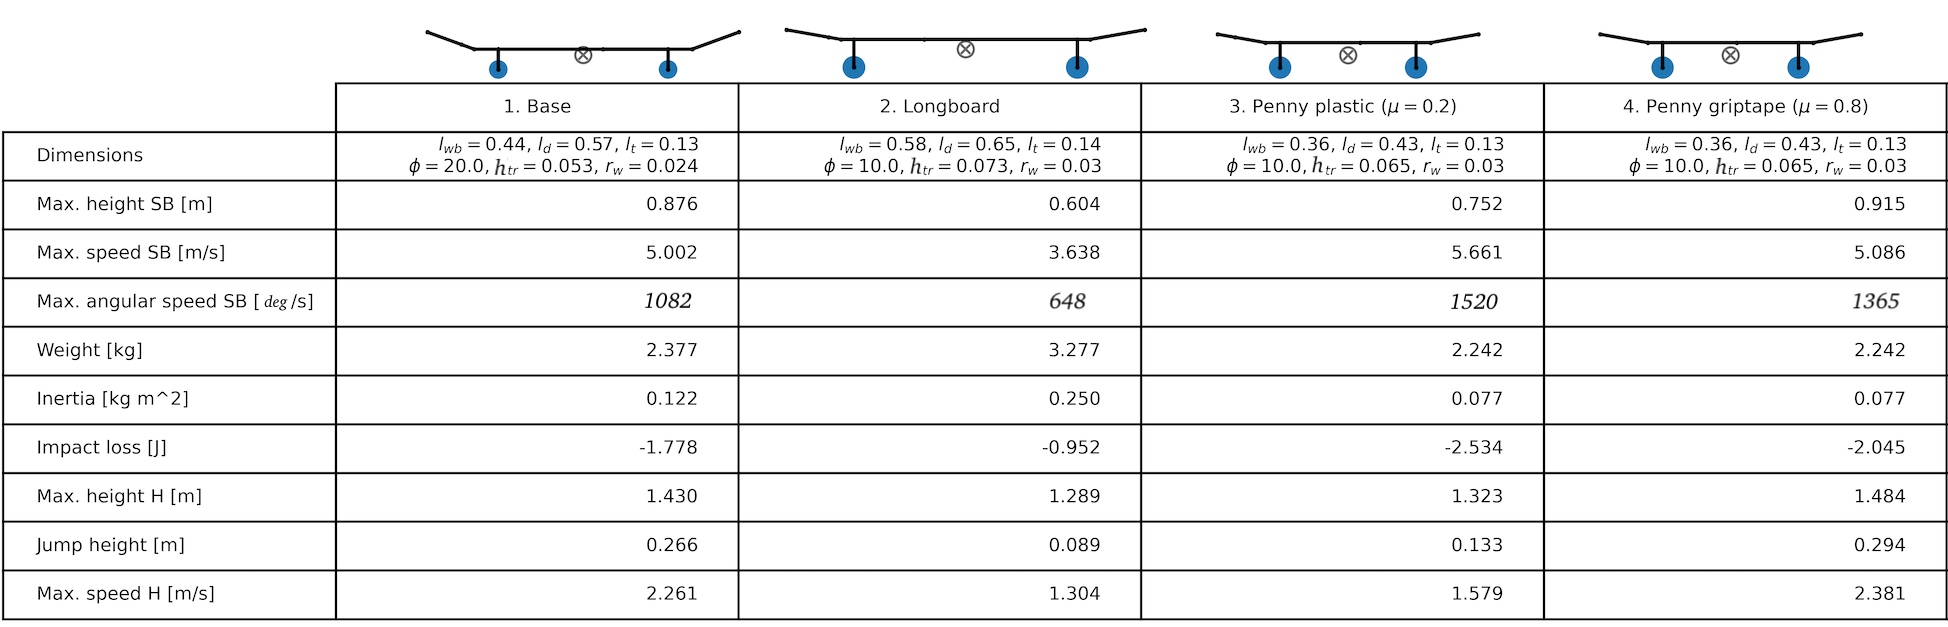
\includegraphics[trim={0 0 0 0},clip,width=\textwidth]{figure/Results/no_optimization_table_dpi600.png}
    \caption[Optimal control  benchmarks for ollie without parameter optimization]{Optimal control benchmarks for ollie without parameter optimization - Schematic skateboard set-ups used to find the optimal ollie. The table shows important benchmarks. Jump height is calculated by minimum vertical position minus take-off vertical position of the person. The impact loss is calculated with kinetic energy of the skateboard after impact minus kinetic energy of the skateboard prior to impact. Other variables are direct output from optimization. }
    \label{f_nopar}
\end{figure*}

\noindent The no parameter optimization was done test the real life scenario that a long board and a penny board are more difficult to ollie. The longboards' dimension are set to an arbitrary OEM longboard.\footnote{\url{https://hlcskateboardfactory.com/ shape: MB701}} The penny boards' dimensions are set to an arbitrary penny board. A penny board is usually made from plastic.\footnote{\url{https://skateboardelite.com/what-is-penny-board/}} The coefficient of friction for the plastic penny is set to 0.2 \cite{bani-hani_data_2019}. For a comparison if the shape of a penny could actually ollie higher a version with griptape is also shown. The three boards are optimized to verify the optimization. Longboard complies with the real life scenario and the optimization shows a 31\% decrease in ollie height compared to the base . The penny board with a plastic top (lower coefficient of friction) is able to ollie 14.2\% lower than the base.

The base skateboard is able to ollie 31\% higher than the long board. The longboards' maximum angular velocity is 40.0\% lower compared to the base skateboard. This is probably due to the fact that the inertia and mass of the long board are higher which will make it harder for the human with limited power to rotate it and get it up. The jump height of the human on the long board is 66.5\% lower compared to the base, meaning that a lot of power is going into the long board instead of jumping up. Resulting in the human mainly to tuck in without jumping). The impact loss is lower for the long board. This could be correlated to the fact that it reaches lower speeds. The contrary is seen with the plastic penny board. It reaches higher speeds and loses more energy during impact. The penny boards are 5.7\% lighter than the base board but have a lower inertia mainly due to the smaller size of the penny board. With a plastic penny board, the human is not able to ollie higher than with the base skateboard. The human jumps 50.0\% and ollies 0.124 [m] lower with the plastic penny board. With grip-tape the penny board is able to ollie higher than the base skateboard. In real life the penny board and long board are harder to ollie. The same is shown in the optimization for the long board. This suggests that the kinetics of the optimization are similar to reality. The penny with griptape is able to ollie higher than the base skateboard, which could have multiple causes. One of them is that a real penny board is made of plastic which deforms more than wood. Which could cause more dissipation of energy and a more difficult control to ollie. The other cause could be that the optimization is lacking kinematic constraints for the human. In real life it is harder to maintain balance when your feet are in a narrow stance. During the balancing narrow stance, in real life it could be more difficult to exert maximal leg power.

\subsubsection{Single parameter optimization}

\begin{figure*}[t]
    \centering
    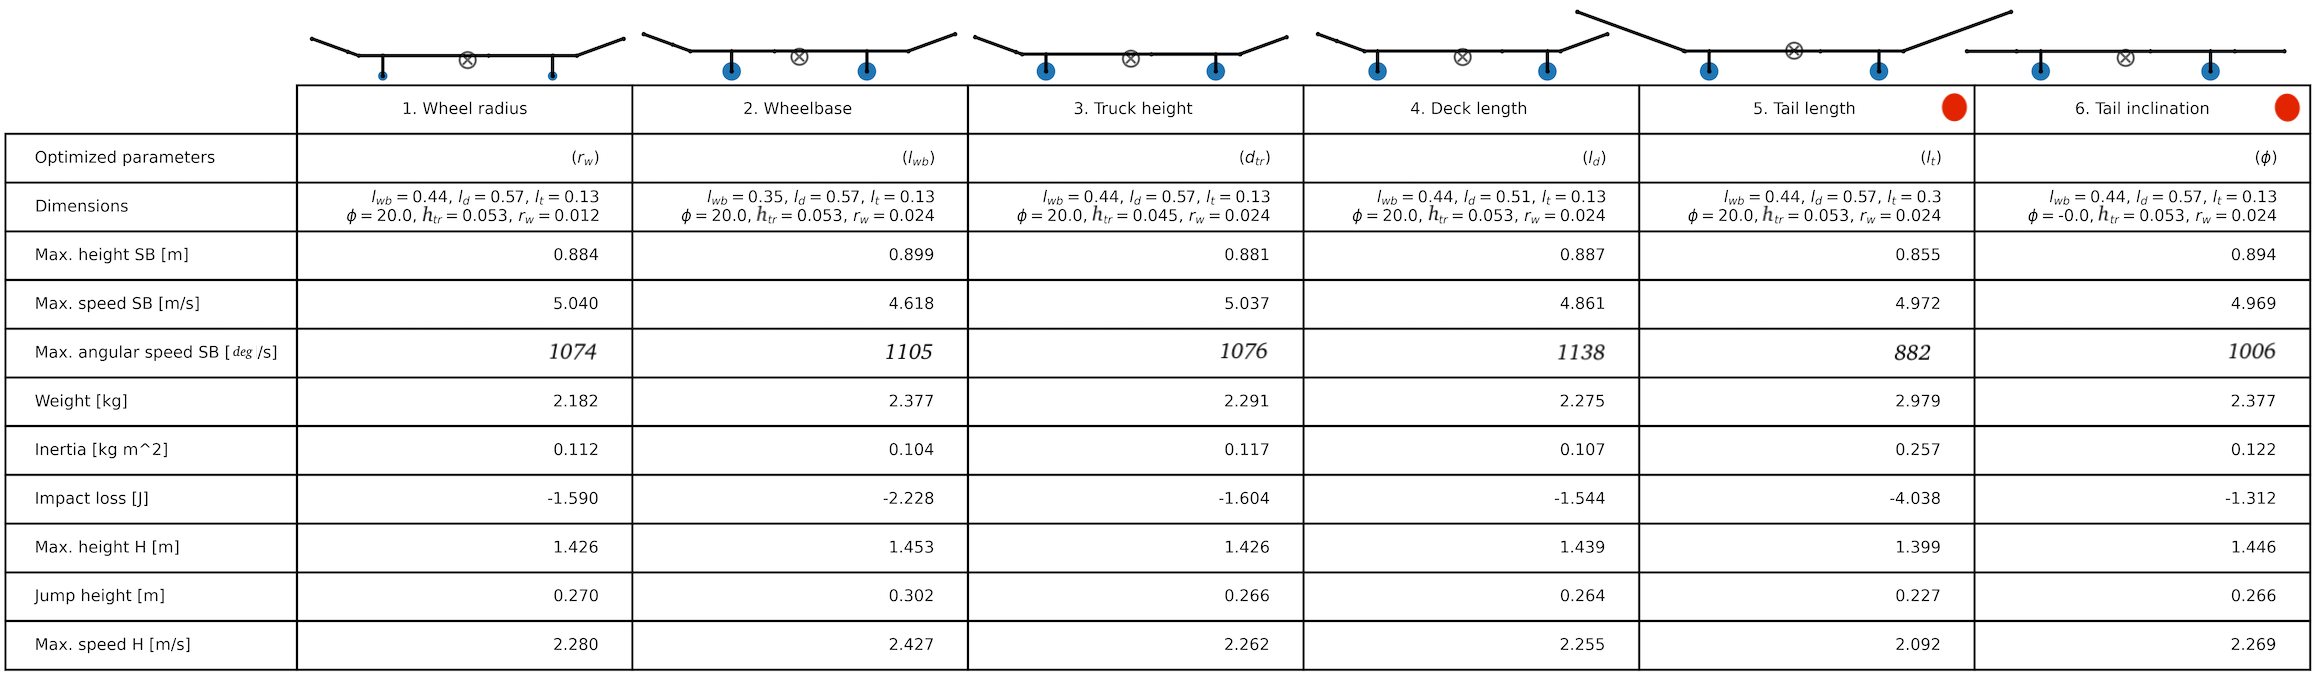
\includegraphics[trim={0cm 0cm 0cm 0cm},clip,width=\textwidth]{figure/Results/single_optimization_table_dpi600.png}
    \caption[Geometry solutions and benchmarks for single parameter optimization]{Geometry solutions and benchmarks for single parameter optimization. The best performing optimization is 2, where the wheelbase is optimized.}
    \label{f_singlepar}
\end{figure*}
\noindent All single parameter optimizations are visible in figure \ref{f_singlepar}. Compared to the base skateboard, all single parameter optimization skateboards were able to ollie higher except for the tail length optimization. The difference in ollie height between the base and the single parameter optimizations is minimal (0.05-0.023 [m]) which suggests that the base skateboard is very close to it's optimum when only one variable can be changed. All single parameter skateboards except for the wheelbase and tail length optimizations show similar human jump height. Which indicates that with these configurations the human is able to exert similar power over time. With a smaller wheelbase the human was able to jump higher. The main differences are found in the weight and inertia reduction which could be the main `drive' of the single parameter optimization. Geometrically the optimizer isn't able to find a large ollie improvement as seen between the base and long board. Still, the optimizer can find a higher optimum by decreasing weight and inertia with all single parameter optimizations except for the tail length and tail inclination optimizations. Which indicates that inertia and weight reduction is a positive influence for ollie height. Dynamically this makes sense because with lower mass and inertia values it easier to lift and rotate the skateboard. The wheel radius, truck height, and tail inclination are hitting the bounds of 0.0125[m], 0.045[m], and 0[deg] respectively, which may indicate a local maxima. Also the tail length optimization did not find a higher maxima than the base optimization which makes it a local maximum per definition, because the base skateboard is a possible solution for this optimization.

\subsubsection{Multiple parameter optimization}
\begin{figure*}
    \centering
    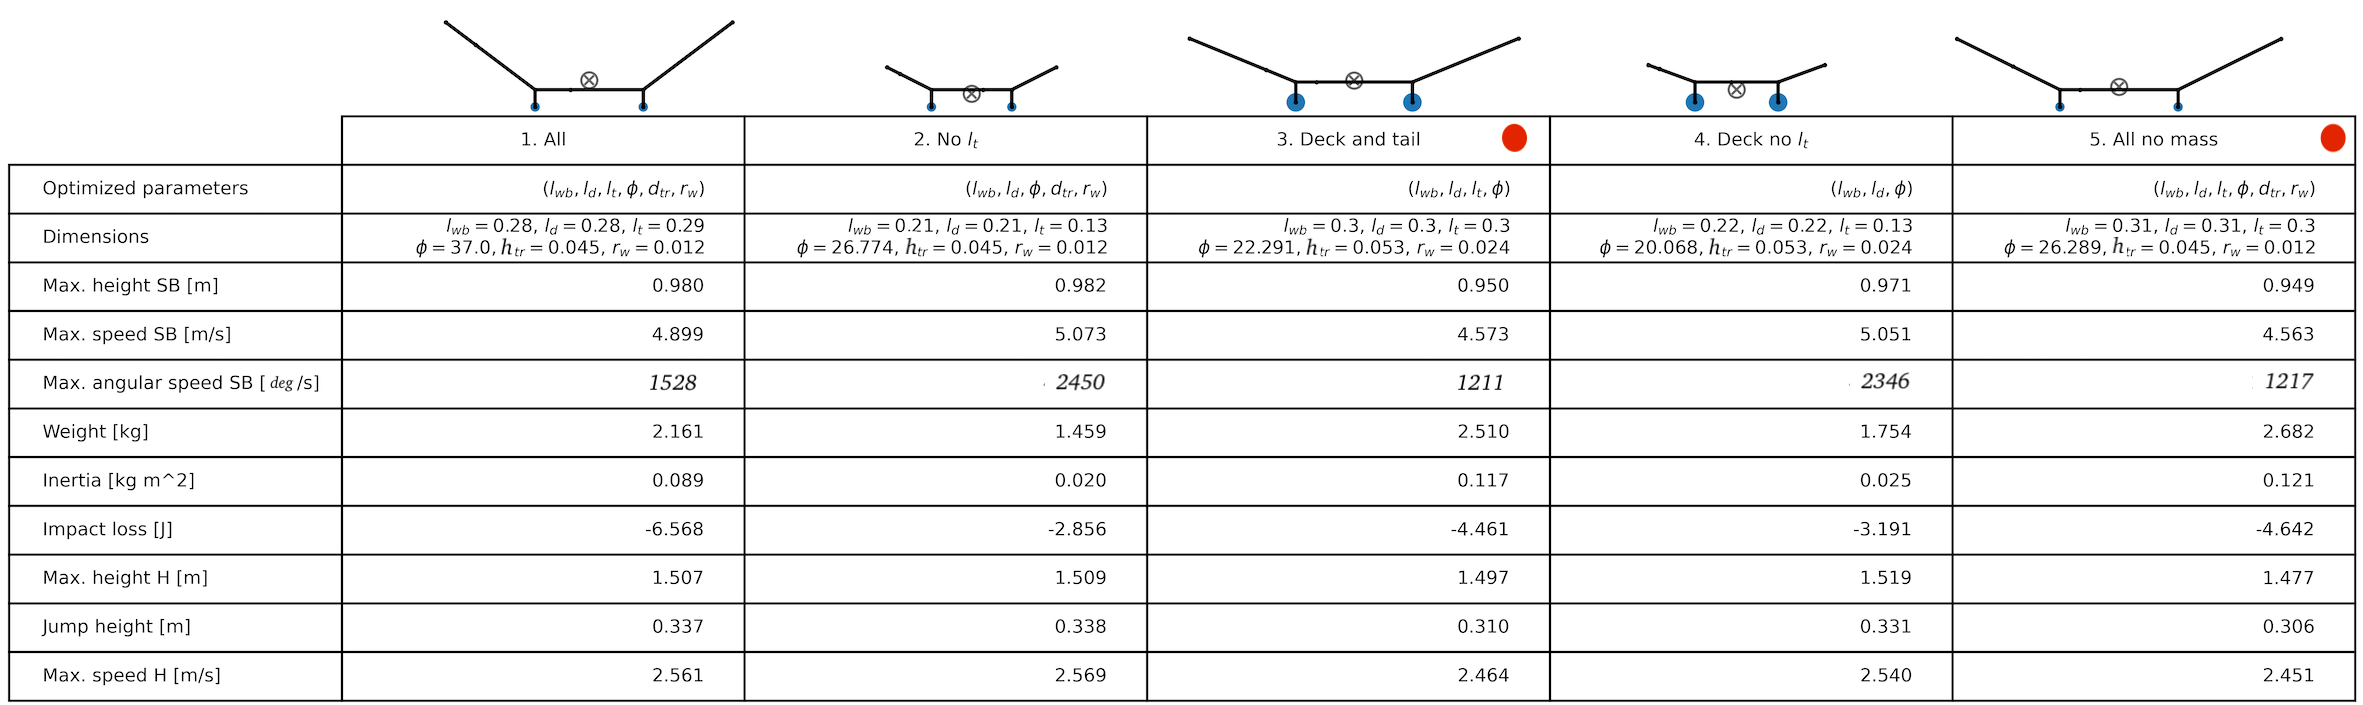
\includegraphics[trim={0cm 0cm 0cm 0cm},clip,width=\textwidth]{figure/Results/multi_optimize_table_dpi600.png}
    \caption[Geometry solutions and benchmarks for multiple parameter optimization]{Schematics of multiple parameters optimizations. Table shows important benchmarks.}
    \label{f_multipar}
\end{figure*}

\noindent All multiple parameter optimizations are visible in figure \ref{f_multipar}. When multiple parameters are optimized the ollie height is improved by 0.074-0.106 [m] compared to the base skateboard. The first column, 'All' in figure \ref{f_multipar} shows the set-up when all parameters are optimized. As seen with the single parameter optimization the tail length is causing strange optima. Once again it is shown that when not optimizing the tail length, the ollie height is higher. This proves that the optimization of all variables is a local optimum, since the optimum found with the `no $l_t$' (figure \ref{f_multipar}) skateboard is a possible solution to the optimization. Same goes for the full deck optimization. The full deck optimization does not optimize wheel radius and truck height. The ollie height for this optimization is 0.021 [m] lower than the same optimization with fixed tail length. This proves that the full deck optimization is a local maxima which is caused by the optimization of the tail length. The cause of hitting a local optimum because of the tail length needs further investigation. When the tail length increases the impact loss increases as well. This is logical when thinking of the tail speed $v = \omega \times r$, which means, the larger the distance between the tip of the tail and COM of the skateboard, the larger the local speed at the tail. The larger the speed at the tail, the more momentum is lost during impact, which is the reason for the higher impact losses. The impact loss is dependant on the mass and speed, the higher the mass or the speed, the higher the impact loss will be. For example in the `no $l_t$' (figure \ref{f_multipar}) optimization the angular velocity before impact is more than twice as high compared to the base optimization. But the mass is also 0,878[kg] less. Thus, the large angular velocity causes the impact loss to be higher, but the mass reduction reduces it, only causing a slight gain in impact loss. 

The most promising optimizations are analyzed further by looking into the states and control over time and compared to the base optimization. The single parameter optimizations show little improvement. The best performing single parameter optimization is the wheelbase optimization with an increase of 2.6\%. The best performing multiple parameter optimization are `no $l_t$' (figure \ref{f_multipar}) (12.0\% increase in ollie height) and deck without tail length (10.7\% increase in ollie height).  All other detailed figures of the optimizations are found in Appendix A. 
\begin{figure*}
    \centering
    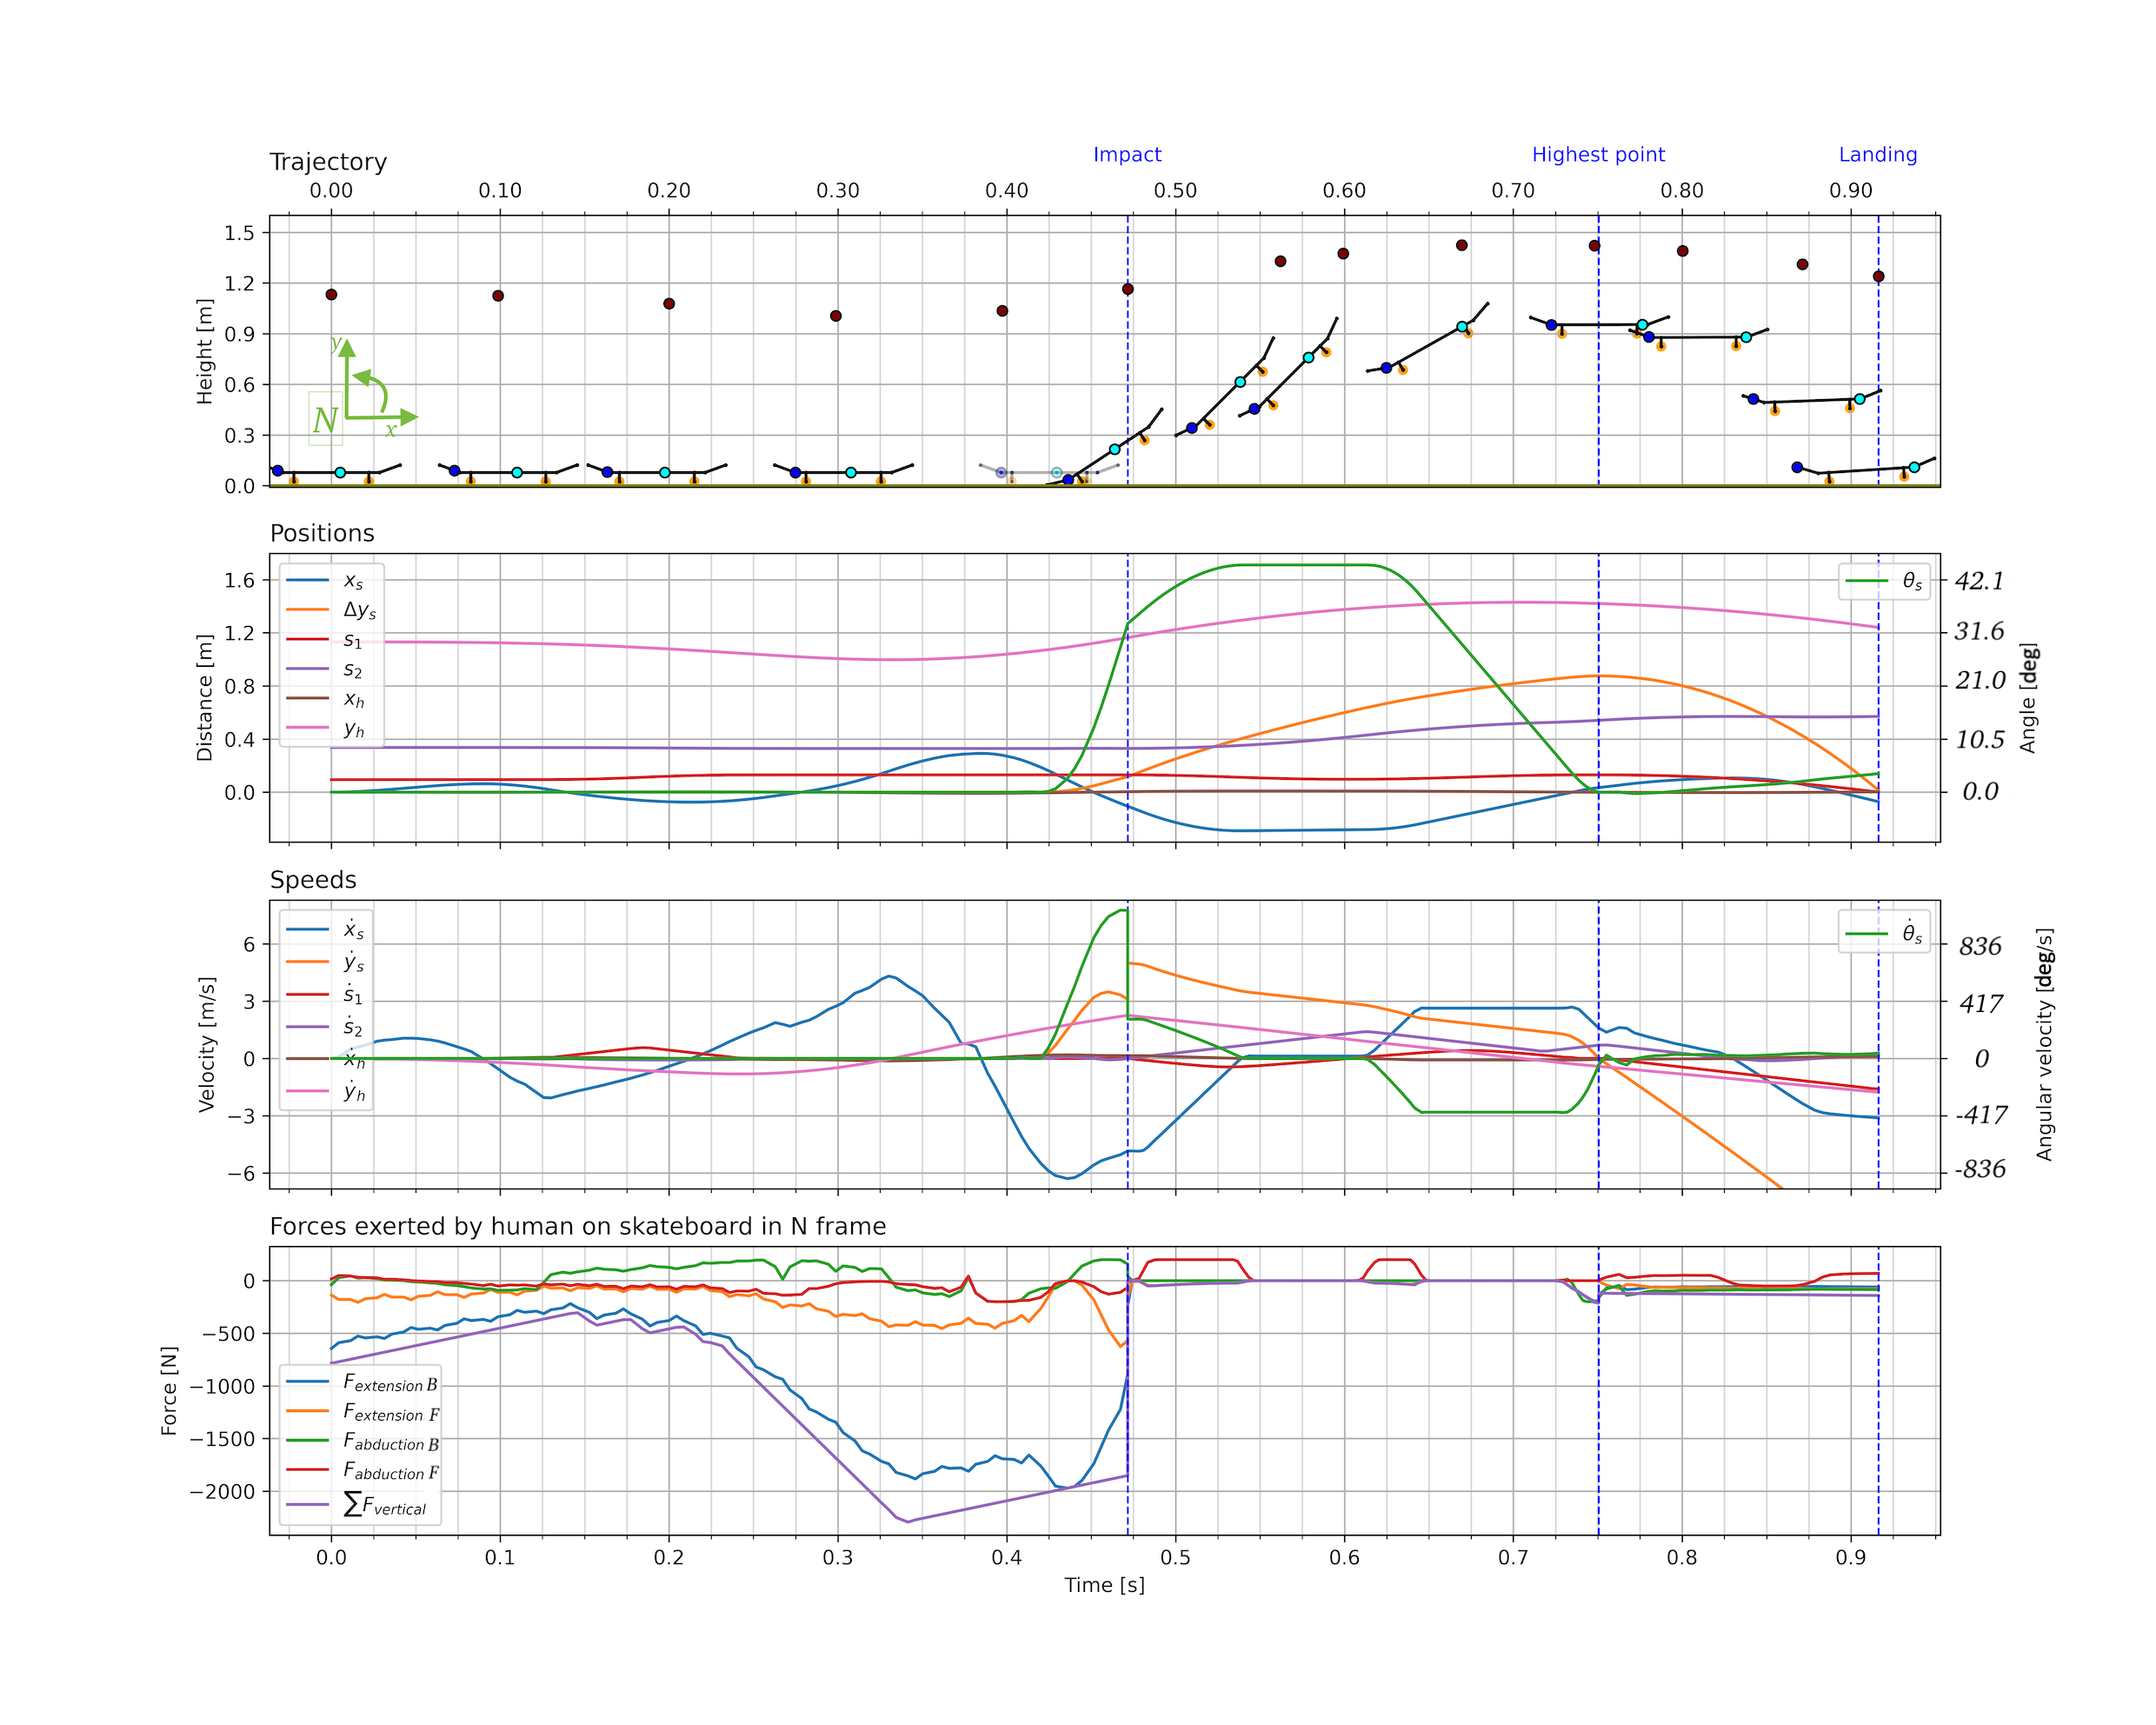
\includegraphics[trim={0cm 0cm 0cm 0cm},clip,width=\textwidth]{figure/Results/data_basedpi600.png}
    \vspace{-1.5cm}\caption[Trajectory, positions, speeds, and forces of base optimization]{Optimization of base skateboard. Corresponds to results in figure \ref{f_nopar}.1. Graph (1) shows the trajectory of the skateboard, (2) are the positions, (3) are the speeds, (4) are the forces. The blue dotted lines are the phase switches. First the human lowers their COM (pink,2) by decreasing vertical force (purple, 4), at minimal human COM height there is maximal force and zero speed (pink,3). Maximal force is almost fully caused by the extension force of the back foot (blue,4). Speed is increased until impact and it reaches maximum speed (pink,3 at impact). Just before impact the skateboard rotates its angle (green,2) from 0 to impact angle. Mid air the speeds are constant except ones effected by gravity (orange,pink,3). The moments forces are exerted the velocities change (t=0.5, t=0.63). The human reaches its highest point before the skateboard. At the highest point force is exerted to `catch' the skateboard. Landing is achieved by stretching and landing on the back wheel }
    \label{f_noparameter}
\end{figure*}
\subsection{Detailed trajectories}
\noindent The results of the optimizations are presented stacked vertically with a shared x-axis which represent time in figures \ref{f_noparameter}, \ref{f_wheelbase}, \ref{f_notail}, and \ref{f_notailnotruck}. The top plots in these figures are the trajectories shown with snapshots at certain time increments. The human centre of mass corresponds with the time of the snapshot. The phase switches are indicated with the blue dotted lines. The positions of the back and front feet are indicated with the dark blue and light blue dot respectively. The second and third plots in these figures are the positions and the velocities respectively. The bottom plots show the forces exerted by the human acting on the skateboard. All states and forces are expressed in the N-frame convention visible in the left corner of the trajectory. The angle and angular velocity are expressed on a second vertical axis at the right of the figures because the units are different from the rest of the states. The forces are presented with the extension force and abduction force. The extension forces correspond to N-frame y direction and abduction forces act in N-frame x-direction as explained in section ref{}. The blue line corresponds to N-frame y-direction leg force acting between the center of mass (red dot in trajectory figure) and the back foot (blue dot in trajectory figure), while the orange line corresponds to the N-frame y-direction leg force acting between the center of mass and the front leg (cyan dot in trajectory figure). The abduction forces are the forces acting between the feet and the COM in N-frame x-direction. For example, before impact, both legs are pushing vertically down on the board, after impact the front foot is pushing sideways in positive x-direction. The sum of the N-frame y-axis forces is presented as the purple line. To see all trajectories that will be presented in the following paragraphs with forces as a video, visit: \url{https://www.youtube.com/watch?v=jw5DmNnvD7c}. In the video static friction and dynamic friction are shown to be performing properly.


\subsubsection{Base skateboard optimization}


\noindent The first figure concerns the optimal control problem without parameter optimization shown in figure \ref{f_noparameter}. The trajectory is very similar to the trajectory seen in figure \ref{f_olliesteps}. Though you have to take into account that this ollie is a standing ollie without an initial horizontal velocity, whereas figure \ref{f_olliesteps} shows a riding ollie. The skateboard relative to the human first moves forward, and just before the impact it rapidly moves backward followed by the tail hitting the ground. The backwards movement happens such that the human can effectively pull the skateboard up and forward with friction and perpendicular force which results in the skateboard being straight under the human at the highest point. The backwards velocity is clearly visible in fig. \ref{f_nopar} speeds, where the blue line before impact is at the largest negative velocity. After impact the velocity will gradually become positive and ending at an almost 0 x position of the skateboard (blue line in positions at second dotted line). If there would not have been a backwards movement, the skateboard would have been pushed out of reach of the human's feet when the board is leveling out. The skateboard is leveled out by a positive abduction force of the front foot (red line forces at $t=0.47-0.55$ and $t=0.62-0.65$). These forces result in a decrease in angular rotation (green line speeds, same time span), and a level skateboard at the highest point (green line positions at highest point = 0).
You can see that the back foot is almost fully located at the pocket of the skateboard. This is the point with the lowest velocity of the tail, the tip of the tail has the highest velocity due to $v = \omega \times r$. When the board is rotating the power that can maximally be exerted by the human legs is limited by the force and the relative velocity: $P_{leg} = v_{rel} F$. This means that if the intention is to jump up as high as possible, the relative speed should be as low as possible, which is why the foot should be in the pocket. When the foot would be on the tip, more distance is lost which could have resulted in a higher jump. 
The impact changes the momentum of the skateboard. In the speeds graph it is visible that the angular velocity at impact vastly reduces (green line, 1082 to 286 [deg/s]), whilst vertical velocity is gained (orange line, 3 to 5 m/s).
The human starts with their knees slightly bent, and having full body weight on the skateboard. In the first phase the human lowers their COM in order to prepare the legs to jump. This is called the unloading phase (from $t=0 - 0.2$). After the unloading phase the force increases. Here the human is braking the downward velocity gained during the unloading phase up until the highest peak of the sum of the vertical forces (purple line). This is called eccentric braking. Then the human vertical velocity (pink line speeds) is at 0 and the human has reached its lowest point. From $t=0.35$ until impact the human is gaining upward speed  (pink line speeds) and reducing the force. The force needs to reduce to comply to the power bound ($P_{leg} = v_{rel} F$). This phase is called the concentric phase. Then the human has lost contact from the skateboard just after impact. Followed by an upward motion gradually decreasing due to gravity, reaching it's highest point just before the skateboard reaches it's highest point. The slopes and maximum of the vertical forces (purple line) are bound by the eccentric RFD(negative) and concentric RFD(positive) and the maximum force permitted. The optimizer is at the bounds and wants to maximize force and power output. The forces are not fully smooth due to the fact that the bounds are on both legs, thus simultaneous counteracting of forces between the front and back leg is permitted in the optimization. Having more kinetic data on single legs could improve this. Also the polynomial to estimate the solution used by the software is not plotted correctly here, so the line should be smoother when using the polynomials used per mesh section provided by the software. Due to practical implications this has not been done. The third reason why the control can be less? smooth is due to the friction constraints. These constraints are difficult to solve and are demanding for the optimizer, which sometimes results in non-smooth forces.
The landing is slightly on the back wheels and the human is almost fully stretched out when landing.

\newpage
\subsubsection{Wheelbase optimization}
\begin{figure*}
    \centering
    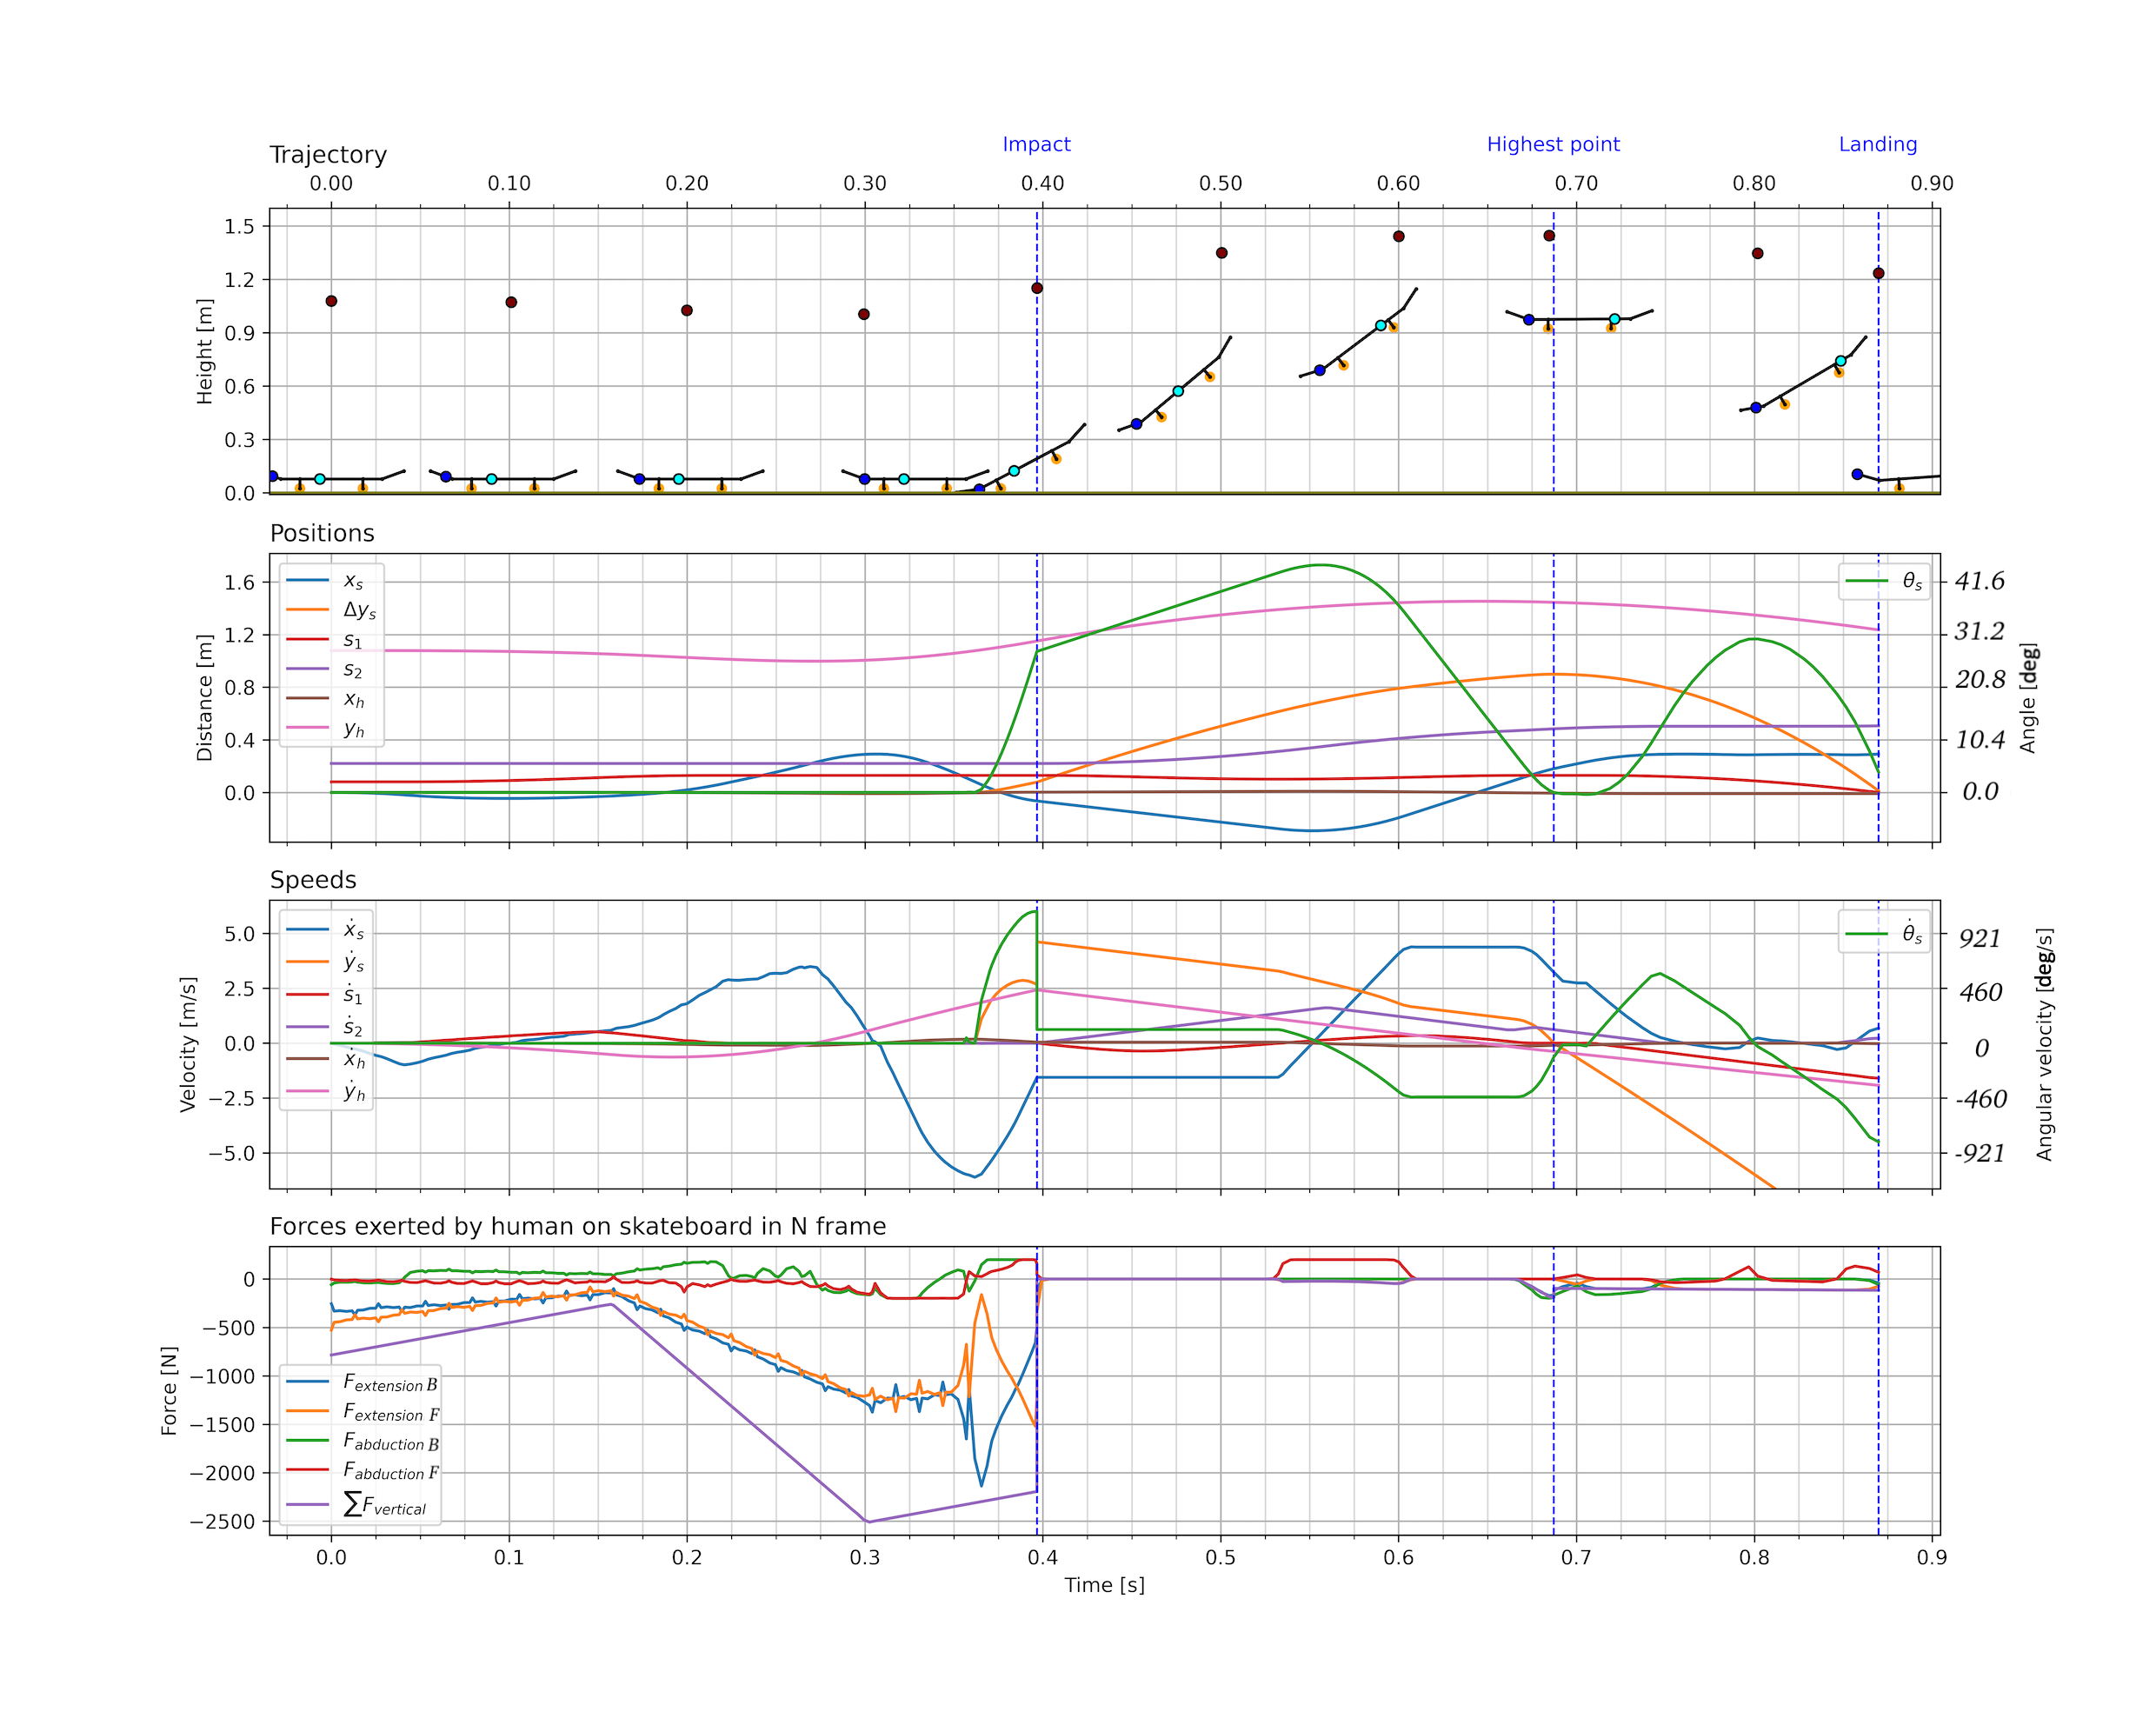
\includegraphics[trim={0cm 0cm 0cm 0cm},clip,width=\textwidth]{figure/Results/data_l_wbdpi600.png}    \vspace{-1cm}\caption[Trajectory, positions, speeds, and forces for wheelbase optimization]{Optimization of wheelbase. Corresponds to results in figure \ref{f_singlepar}.2. 0.09[m] smaller wheelbase compared to base, 0.023[m] higher ollie. Three striking differences, the first is that the jumping force is now equally dependant on the back and front extension force (blue,orange,4), the second is that there is only one force peak between impact and highest point. The third striking part is that the skateboard rotates before landing (t=0.8).}
    \label{f_wheelbase}
\end{figure*}
\noindent The next optimization concerns the single parameter optimization shown in figure \ref{f_wheelbase}. The wheel base of the skateboard will be optimized along with optimal control. The performance of this skateboard has been discussed in figure \ref{f_singlepar}. This skateboard was able to ollie 0.023[m] higher than the base optimization. Most of the phenomena seen in the base optimization are also visible for this optimization. The human lowers their weight, pushes the skateboard forward then pulls it backward. Angular velocity is lost during impact (-1193 [deg/s] and vertical speed is gained (green and orange lines speeds). After impact abduction force with the front leg is used to pull the skateboard up and level it out. The first difference is visible in the force plot. The sum of the vertical forces (purple line) does not stagger when unloading. A straight line up, down, and then up is achieved. Secondly, a higher angular velocity is achieved compared to the base. The back foot is once again in the pocket of the board, but now the front foot is at equal distance from the wheel having perfect balance. At this position both legs can exert equal force without rotating the board during eccentric braking ($t=0.15 - 0.3$). Then suddenly shortly before the impact, the front foot (orange line forces) pulls up and the back foot pushes down to create a maximal momentum about the back axis creating a steep sudden increase in angular velocity. The decreased wheelbase causes the impact angle to be lower and the angular velocity near zero just after impact (green lines positions and speeds). This leaves a period of rest such that the skateboard can gain height. While the front foot is in a sliding motion, the foot starts pushing down on the board at t=0.53.  This is almost enough to level the board out at the highest point. But the negative angular rotation caused by this push is caught with the back foot at the highest point making sure the board is leveled. 
The reason why this board can ollie higher is because it needs less control during the upward motion to level the board out and is able to reach higher angular velocities due to reduced inertia. By decreasing the wheelbase, the inertia of the skateboard is decreased. With a decreased inertia, the dynamic response is faster resulting in higher angular velocity with the same amount of torque produced. Also less force is needed to level the skateboard during the upward motion because the same amount of force input will result in a larger angular deflection compared to the base skateboard. 

\begin{figure*}[t]
    \centering
    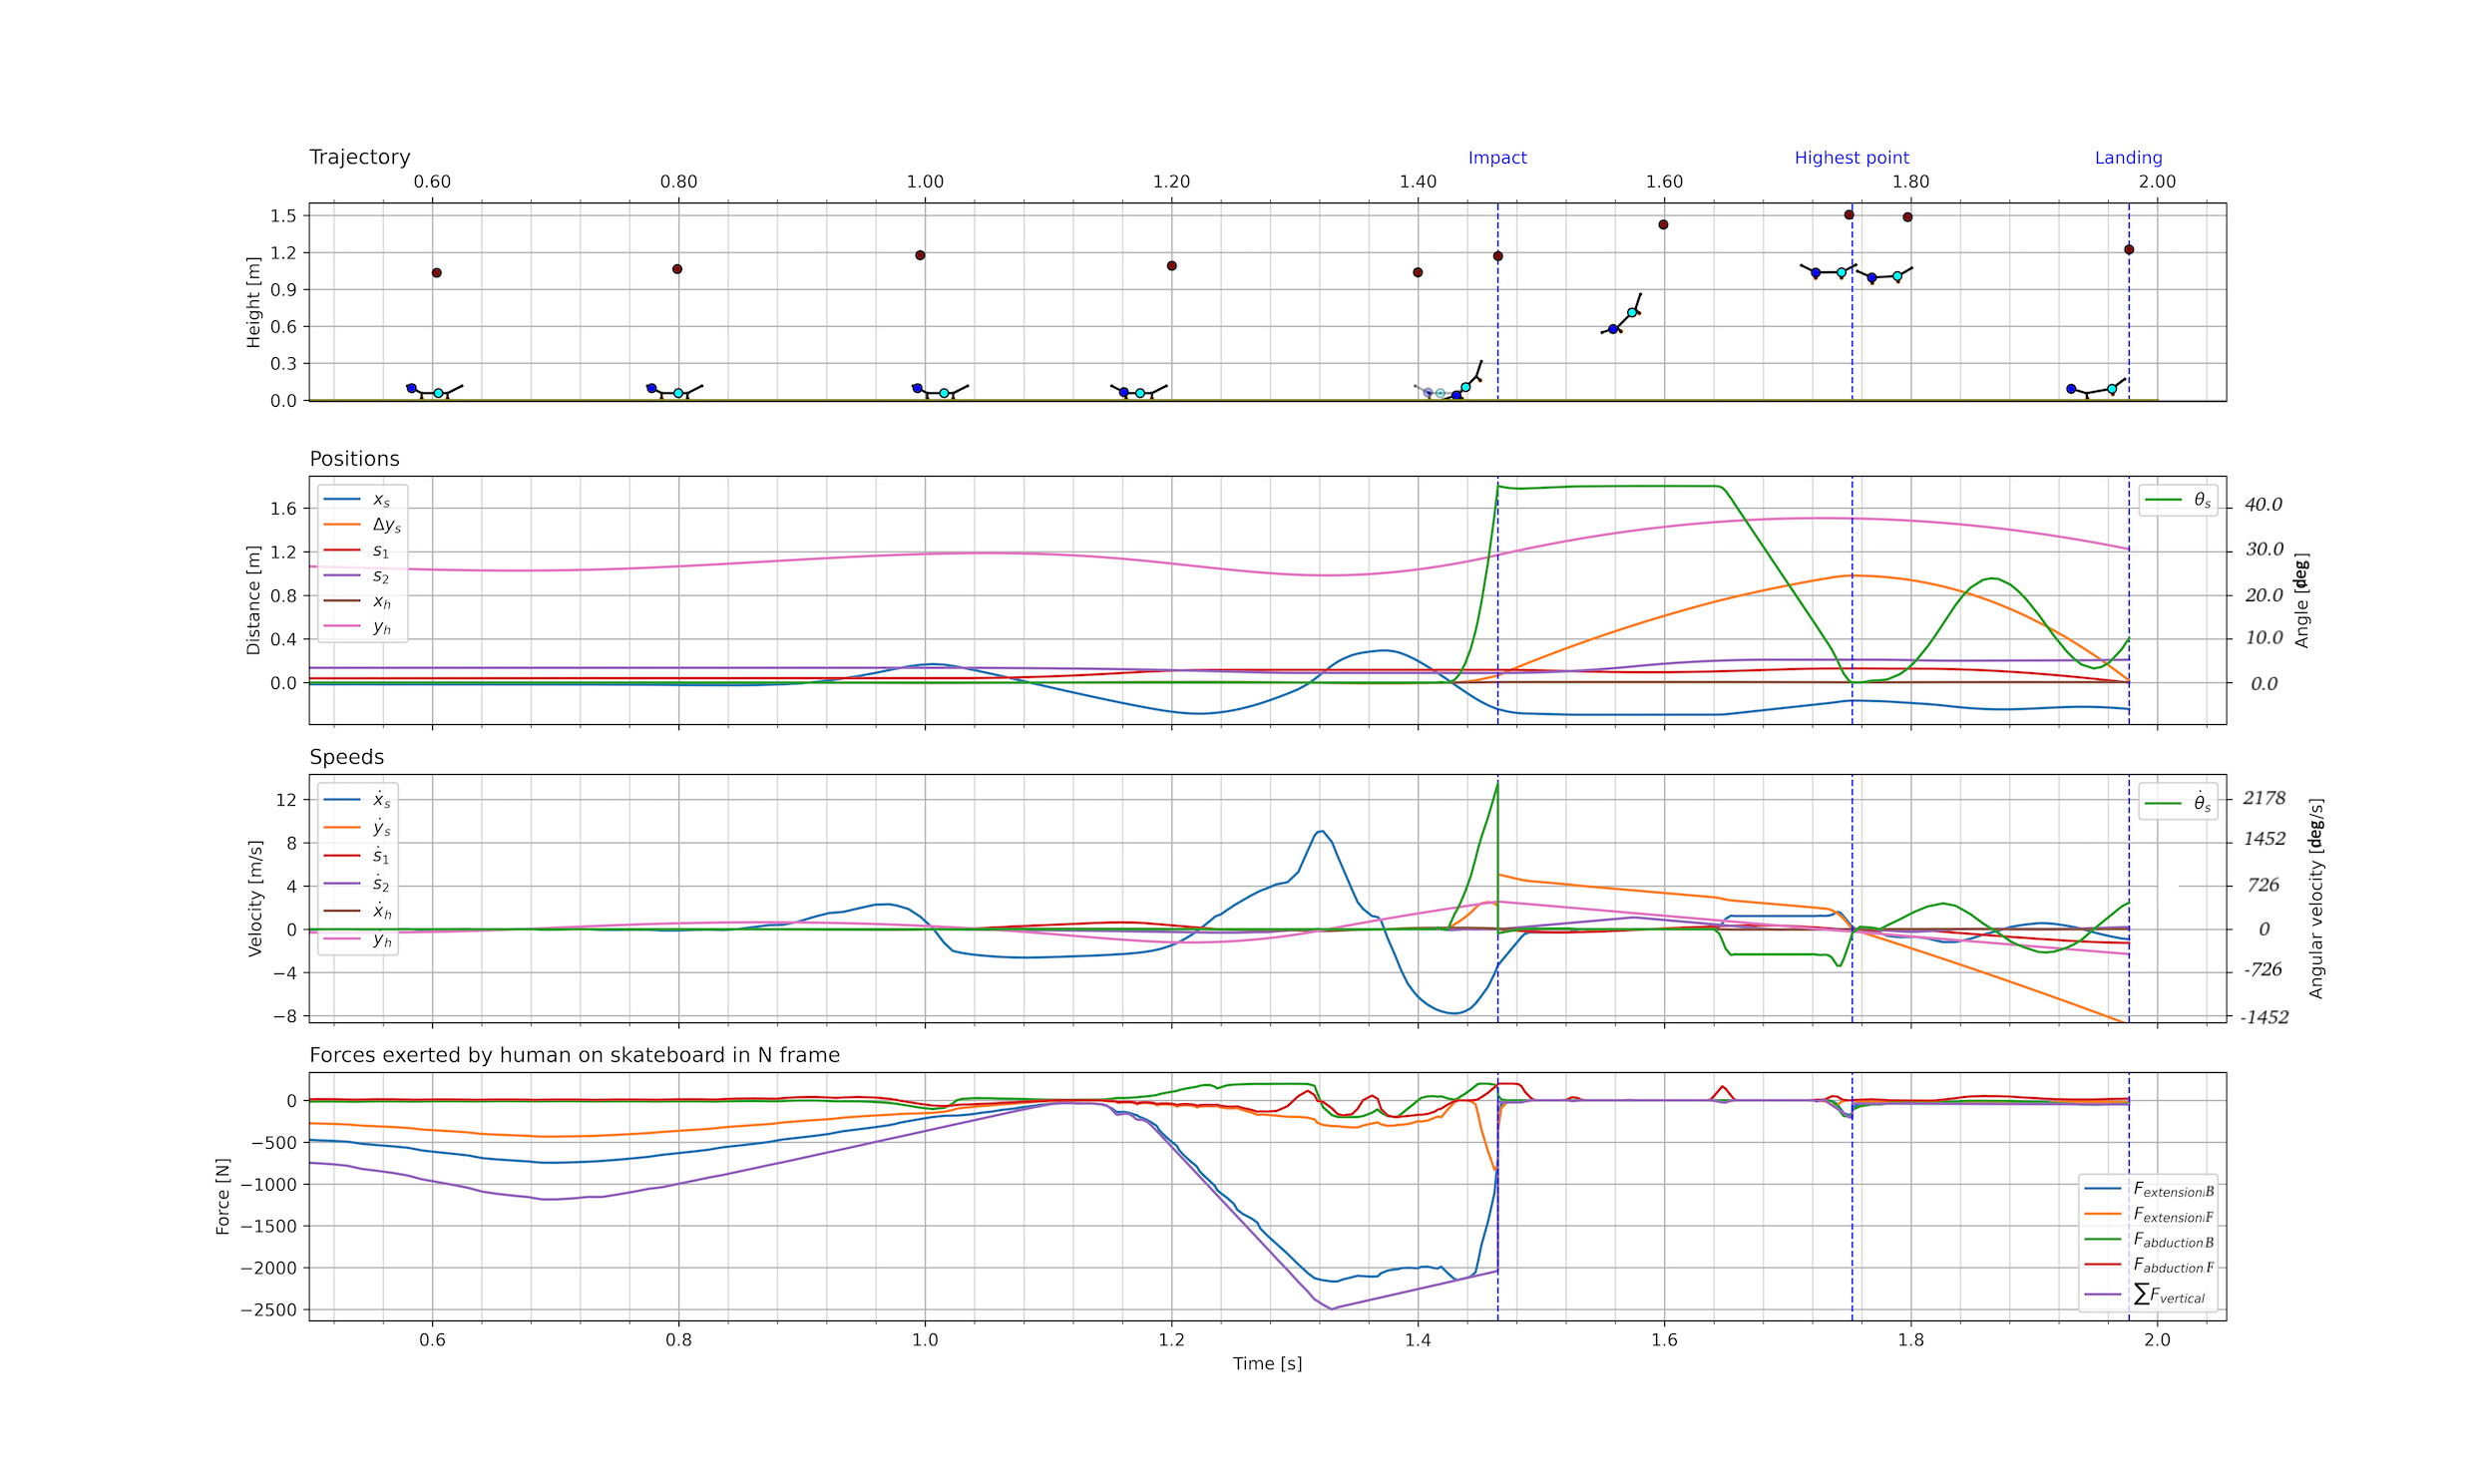
\includegraphics[trim={0cm 0cm 0cm 0cm},clip,width=\textwidth]{figure/Results/data_no_taildpi600.png}
    \caption[Trajectory, positions, speeds, and forces for `all except tail length' optimization]{Optimization `no $l_t$'. Corresponds to results in figure \ref{f_multipar}.2.}
    \label{f_notail}
\end{figure*}
\begin{figure*}[t]
    \centering
    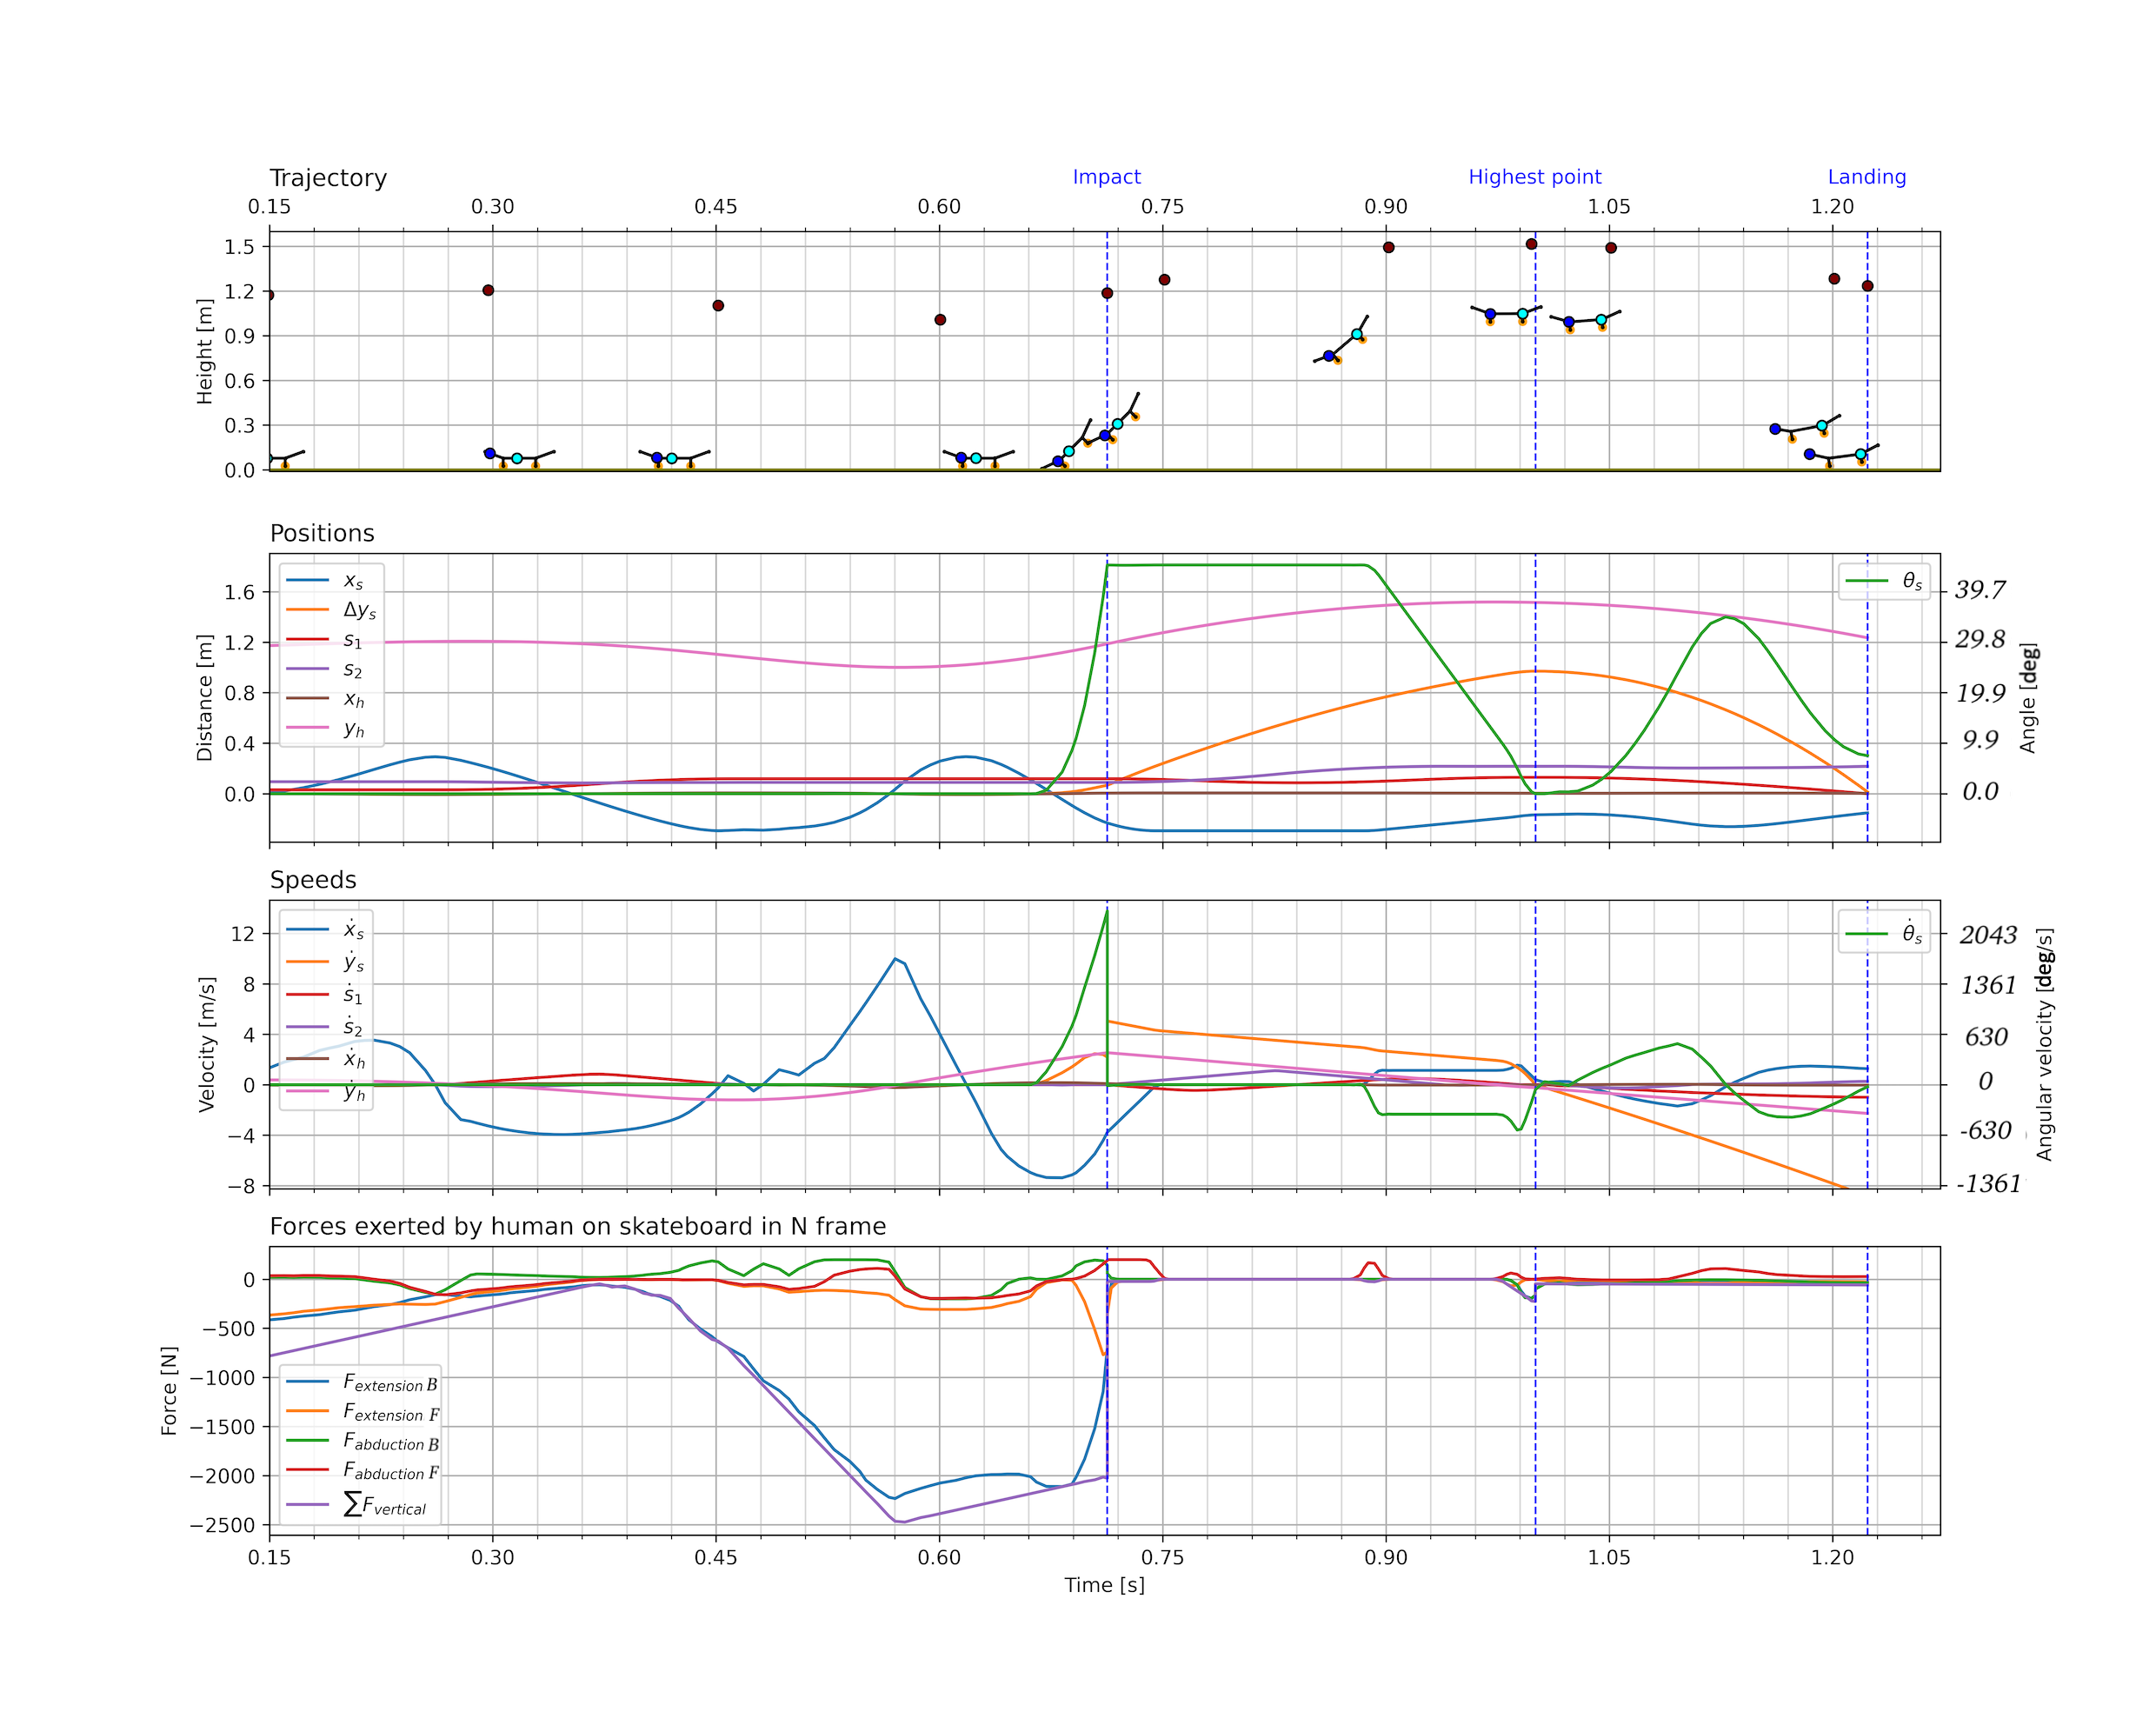
\includegraphics[trim={0cm 0cm 0cm 0cm},clip,width=\textwidth]{figure/Results/data_notrrwltdpi600.png}
    \vspace{-0.5cm}\caption[Trajectory, positions, speeds, and forces for `deck except tail length' optimization]{Optimization `deck no $l_t$'. Corresponds to results in figure \ref{f_multipar}.4. The human first goes up and down before wanting to jump (pink,2). The time before impact is (long 1.46 [s]). The rotational speed at impact is 2178 [deg/s]. Between t=1.5 and t=1.8 there is almost zero force exerted, a small peak at t=1.7 is sufficient to level skateboard at highest point. At highest point the skateboard is behind the human. }
    \label{f_notailnotruck}
\end{figure*}

\subsubsection{Multiple parameter optimizations}
\paragraph{All except tail}
\noindent In this optimization all variables but the tail are optimized shown in \ref{f_notail}. Compared to the base skateboard, this skateboard is able to ollie  higher (0.106 [m]). Though a lot of similarities can be found between the two. The horizontal velocity is negative prior to impact, than after impact the board is dragged upward and forward. This skateboard is significantly easier to rotate due to the lower inertia and mass ($I_s = 0.02 [kg m^2]$ compared to $0.122 [kg m^2]$ for the base skateboard and $m_s = 1.459 [kg]$ compared to $2.377 [kg]$ for the base skateboard). Due to these lowered variables, with the same amount of force over time the angular velocity that is obtained is twice as high. (green line speeds). It is worth noting that the human jumps highest with this skateboard setup. 
With this setup the skateboarder is able to jump almost solely from its back foot (blue line forces) due to the fact that the foot is located almost exactly above the back wheel such that there is no or little momentum created about the back axis. 

\newpage

\paragraph{Wheelbase, tail inclination, and deck length}
\noindent In this optimization the truck height and wheel radius are not optimized as shown in figure \ref{f_multipar}. The trajectory, positions and speeds of this skateboard are very similar to the prior optimization. The mass and inertia have increased due to the higher weight of the wheels compared to the previous optimization. The wheelbase and tail length came out to be the same length as the .


\newpage
\section{Discussion}
\noindent The skateboard trajectories are all very similar to an actual ollie. Without any motion cues, the optimizer is able to replicate the ollie motion, with almost all phenomena seen in \ref{f_olliesteps}. The optimizer shows that the human first jumps, then slams the skateboard to the ground, slides the front foot over the deck to drag it up and level it out and catches the skateboard with the back foot at the highest point. This is very close to reality. The human replicates the counter movement jump with a very similar force graph if figures \ref{f_notail} and \ref{f_GRF} are compared. Also the impact energy is similar to the impulse found in figure \ref{f_GRF}. The impulse from the GRF is roughly 5 [J], which is of the same order of magnitude as the found impact losses in figures \ref{f_nopar}, \ref{f_singlepar}, and \ref{f_multipar}.
A single mass point with two free floating feet controlled by forces and feet location with kinematic constraints are able to simulate the motion and output of a human jumper. 
Nine out of eleven optimal skateboard geometries found higher ollies compared to the popsicle stick skateboard. None of these solutions is proven a global optimum, but the improvement to the base skateboard is something that performs better. Skateboard builders should try to implement found geometries and test empirically if they will improve ollie height. These geometries could be a tool to alter existing skateboards and let athletes jump higher. The kinetic and kinematic constraints are of a specific person. The geometries might be dependent on the human capabilities. Empirical testing is necessary to prove that this finding is true in a real life ollie. I successfully solved the ollie optimization problem with a geometry optimization. Compared to others Shield et al. \cite{shield_contact-implicit_2022} who solved an optimization problem for the ollie, my optimization was faster (3 min vs. 43 min), included an geometry optimization, and had a more difficult objective function. The Shield optimization was was set at a fixed ollie height and needed motion tracking to solve optimally. My optimization had a null seed initial guess, with an objective function that maximized ollie height. Such objective functions are generally hard to solve, for example in \cite{nitschke_efficient_2020} first tracking data needs to be implemented to solve a more difficult objective. Step by step less data can be used to solve for an more difficult objective. In the case of this paper, the solution is found without any tracking data and a difficult objective function. 
\subsection{Findings}
\noindent\textbf{Lower inertia and skateboard mass is beneficial for ollie height.} In all parameter optimizations that improved ollie height compared to the base, a reduction in mass and inertia is found. This is logical when looking at the Newton-Euler equations $Force = Mass \times Acceleration$ and $Moment = inertia \times angular acceleration$ The lower the mass, the higher the acceleration the easier the skateboard can go up. With lower inertia the skateboard rotates more easily which minimizes the amount of force needed with the leveling out of the skateboard during upward motion. If that amount of force is lower, the skateboard is pushed down less, which results in a higher ollie. 
   % IF THESE SOLUTIONS ARE GLOBAL OPTIMA
   
\noindent\textbf{Popsicle stick skateboard is close to optimum and slight changes due to preference will not influence the ollie height too much.} As seen with the single parameter optimizations the increase in ollie height was minimal (0.05-0.023 [m]). Only when multiple parameters are changed the ollie height increased significantly (0.074-0.106 [m]), but the shapes are completely different from a popsicle stick skateboard. If skateboarding will keep the popsicle stick skateboard as standard due to the fact that other tricks need to be performed other than the ollie, not much can be changed to the skateboard to optimize it. If the skateboard will change completely, the ollie height could be improved. The wheelbase effects the ollie height the most of all single parameter optimizations, which could be a promising outcome since it does not influence the board shape which is crucial for other tricks. 

\noindent\textbf{Extremely fast optimal solution is found and easy convergence.} The ollie optimization by Shield et al. \cite{shield_contact-implicit_2022} was without a parameter optimization of the skateboard. This optimization took about 43 minutes to solve, and accurate initial guesses were needed for feasible results. The full code presented by me took under 3 minutes to solve. This includes derivation of the Equations of Motion and all constraints, the time to transcribe the problem and to solve in IPOPT. This was all done without initial guesses and solved optimally.


\noindent\textbf{Optimal back foot position is influenced by the leg characteristics of the performer.} In all optimizations the back foot is sitting in the pocket of the skateboard. For example imagine a simple lever system with a fixed force magnitude perpendicular to the lever with distance x from the rotation point. The higher x, the more torque can be generated, but the greater the distance ($s$) the force will travel. In other words $P = F \delta s = F v $. With a fixed power there has to be a trade of between force and velocity. In this case velocity of the back foot is minimized by setting the back foot in the pocket. According to a jumping theory by Morin an Samozino \cite{morin_biomechanics_2018}, jumping output is bound by a force velocity curve, where maximum force can be exerted at zero speed and maximum velocity at zero force. Athletes have different force velocity profiles where one prefers high force output over high velocity and vice versa. The controller preferred the force profile by minimizing the back foot velocity. This finding leads to the conclusion that athletes with different leg profiles should place their feet differently during the ollie. Where a force-profile should set the back foot in the pocket and a velocity-profile on the tip of the skateboard. See figure \ref{FVcurve} for force and velocity oriented human leg output.

\begin{figure}
    \centering
    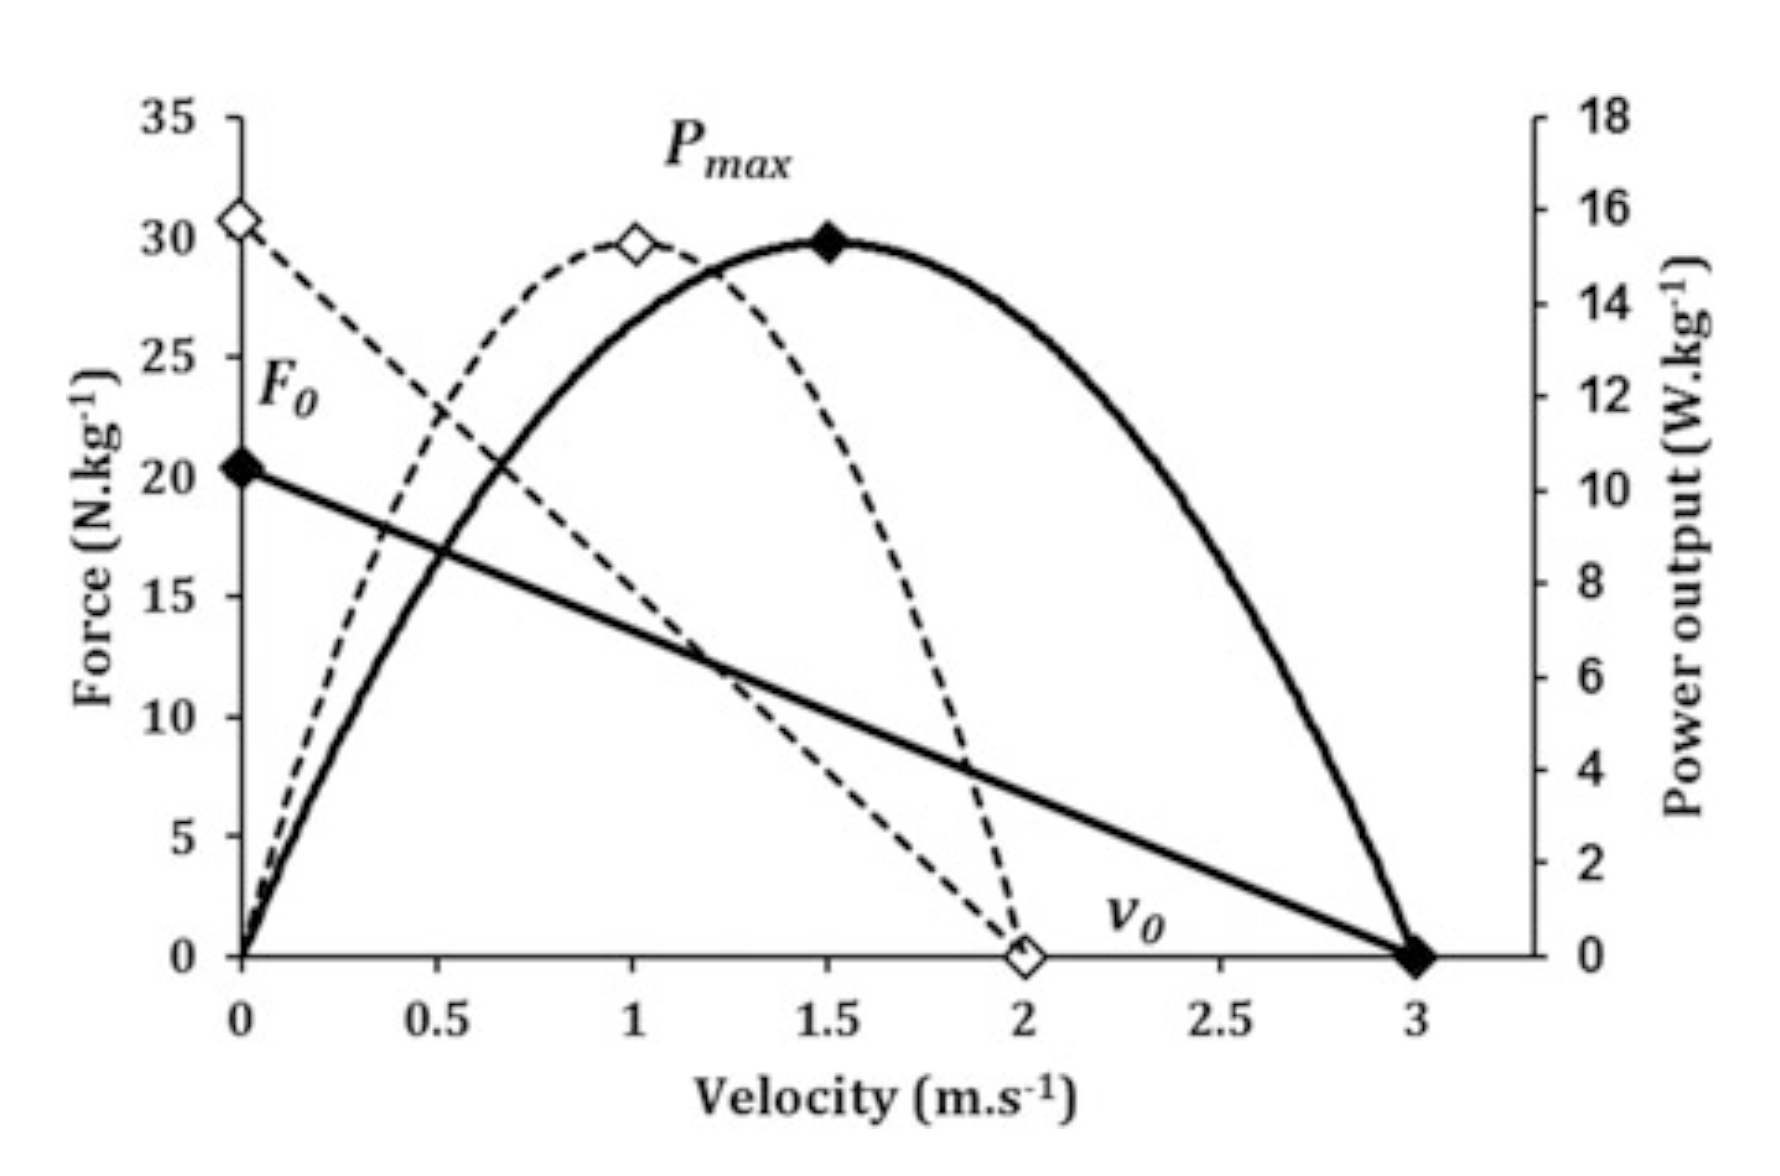
\includegraphics[width = 0.4\textwidth]{figure/Schermafbeelding 2022-11-21 om 16.08.08.png}
    \caption[F-v curve]{Theory on human leg output during jumping. When increasing the load, the maximal force and velocity stay on the line. The dotted line shows a more force oriented human, whereas the other shows a more velocity preferred human jumper. Both have the same maximal power output}
    \label{FVcurve}
\end{figure}

\noindent\textbf{Highly adoptable model.} The presented model can be adjusted to the kinetic and kinematic bounds with little effort. The possibility to optimize a skateboard for a specific athlete is not hard to implement but the kinetic data should be present. Also preference bounds such as width are easily implemented.

\noindent\textbf{Inertia and mass model inertia and mass model for a skateboard is presented that can estimate the dynamic board behaviour in 2D}. The model should be verified with multiple skateboard geometries.

\noindent\textbf{Well represented kinetics.} All results show high similarities between the force profiles of the counter movement jump seen in figure \ref{f_cmj}. The sum of the human kinetics are well bound and show constant results. Even though it is a highly simplified model, the output of the forces is very similar to the output of a CMJ. The point mass model is insightful for the dynamics and is able to show valid results. \\

\noindent\textbf{A fundamentally different simplified contact implicit optimization is made.} The relaxed formulation by Patel et al. \cite{patel_contact-implicit_2019} has been simplified by restating the contact definition. Static and dynamic friction is achieved with the ability to have contact implicit events.

%This book has a chapter about practical implementations on estimating the ballistic performance. The theory says the legs can only produce a certain force at a certain speed, which gives a straight line between the maximum velocity and maximum speed (see fig. \ref{fv}). F0 represents the maximal external force lower limbs could produce during a theoretical extension movement at null velocity. v0 corresponds to the maximal velocity at which lower limbs could extend  under zero load. The values for F0 and v0 are taken from a theoretical optimum for jumping under an angle at 90 degrees with a jump height of 50 [cm] and a maximum power output of 40 [W/kg] at degrees giving: $F0 = 3200 $ and $v0 = 4$. \

% \begin{figure}
%     \centering
%     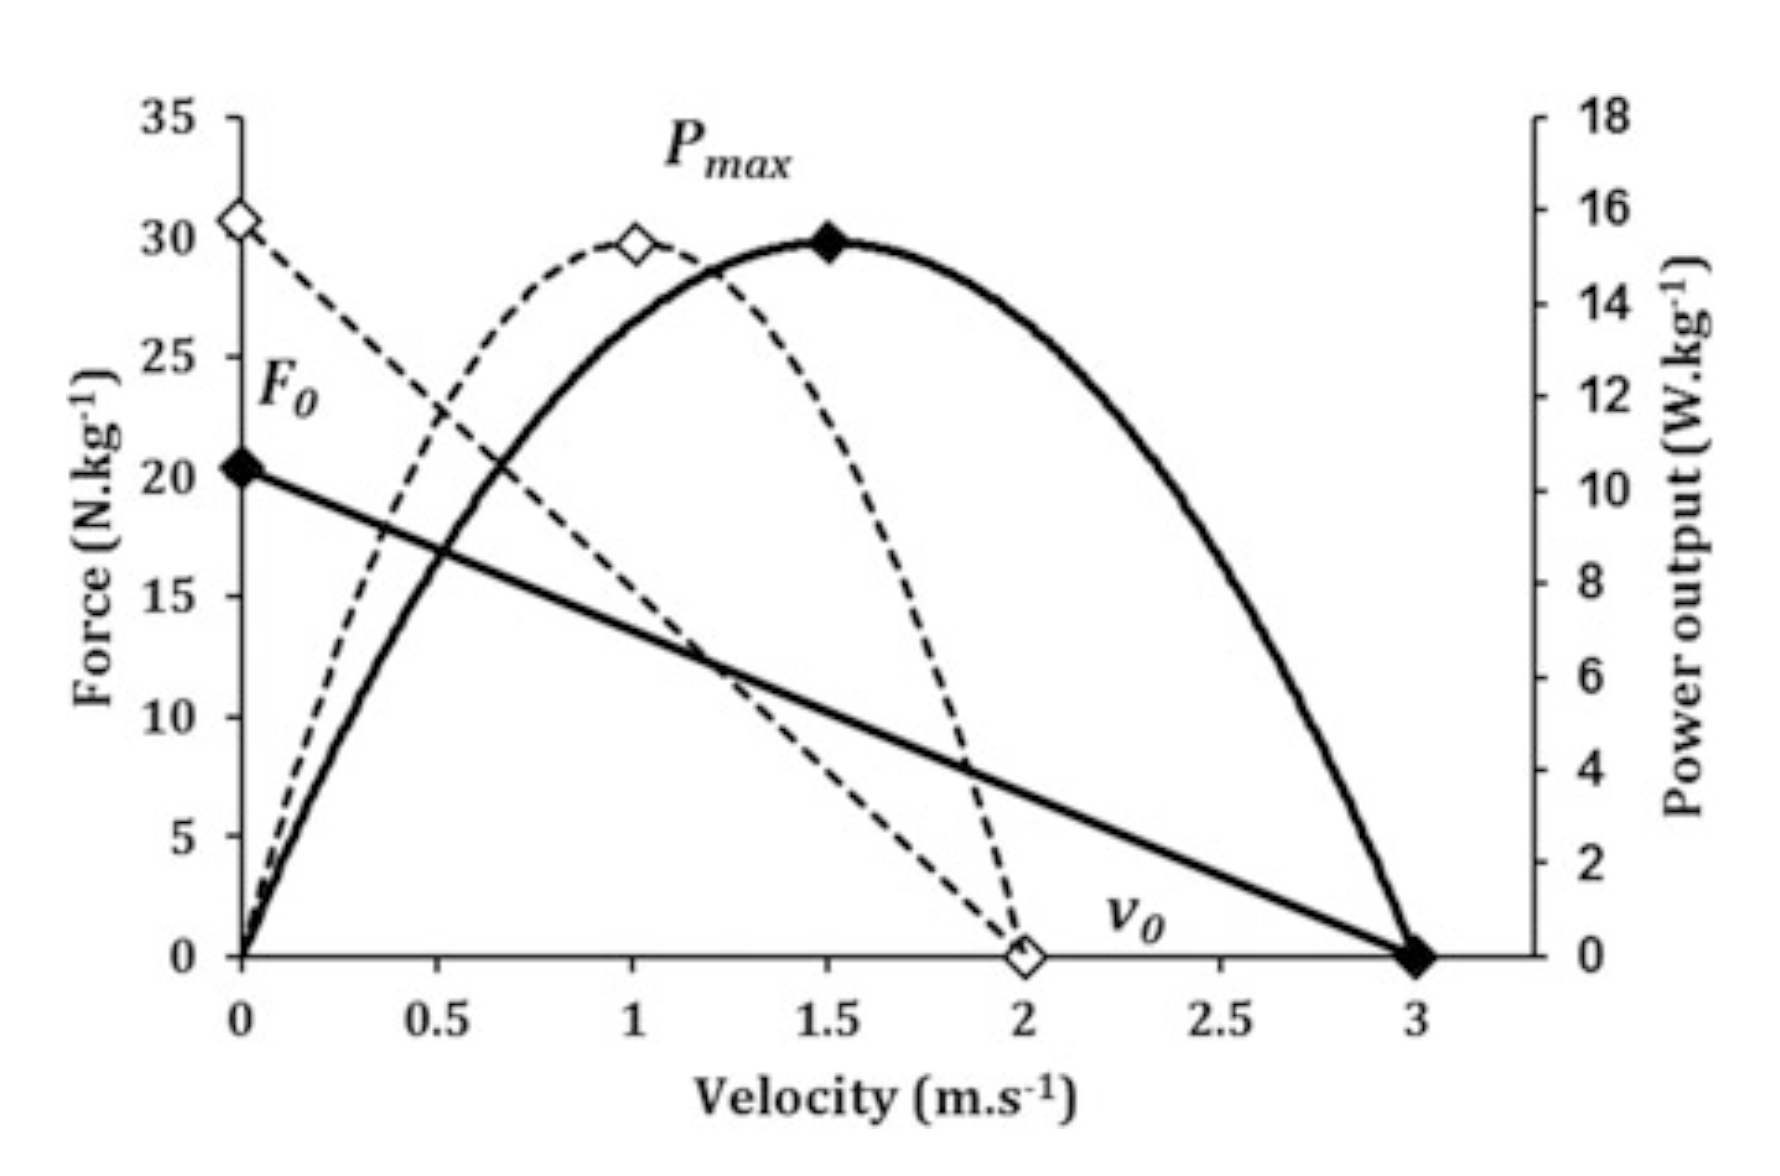
\includegraphics[width = 0.5\textwidth]{figure/Schermafbeelding 2022-11-21 om 16.08.08.png}
%     \caption{Force velocity curve and power}
%     \label{f_fv}
% \end{figure}
\subsection{Limitations and Future research}
\noindent\textbf{Tail length optimization leads to local maxima.} As seen in the results the tail length optimizations showed lower ollie height compared to the same optimizations with restricted tail length. This is per definition a local maximum because the solution space of the optimization with tail length optimized should contain the restricted tail length optimization solution. In real life a longer tail length would cause a higher energy dissipation due to more bending during impact \cite{stronge_impact_2000}. A plausible cause for these local maxima is that impact loss is of too little effect. When a human jumps, the order of magnitude of the amount of energy necessary to go up is in the order of $10^3$. The dissipation of energy during impact is in the order of $10^{-1}$. This means that the impact loss could be of so little effect to increasing ollie height that the solution space has become very flat. You can see that the model does capture the increase impact loss. When the tail length is optimized and the large tail length solution is found, there is an increase of 227\% compared to the base optimization. Maybe if the impact loss would be penalized more, optimal tail lengths will be found.
 
% Range of motion, balance, spacial skeletal constraints
\noindent\textbf{Lack of complexity in the kinematic constraints of the human controller.} Due to the simplification of a human as a mass point with two feet, kinematic constraints are highly simplified. In real life a penny board is difficult to ollie due to the fact that the operating area is really small. The feet would have to operate precise and powerful movements while balancing on a small surface. While the controller can easily do this, it does not represent reality completely. Also inertia of the human is neglected due to the simplification.

\noindent\textbf{Front wheel normal force.} In future research it is advised to implement a normal force acting on the front wheel during the preparation phase. The front foot had to counteract the rotation created by the back foot. In real life the front foot could have been on any location without causing a counter clockwise rotation due to the compensation of the normal force. Difficulties will be to find a phase switch cue for the optimizer. It might be possible to set a fixed time for the first phase to solve this.

\noindent\textbf{Possible that current solutions are not global optima, more optimal board shapes can be found.} The presented solution space is very large due to many possibilities in variables. In future research, many more geometries can be found which could help the skateboard community to understand the dynamics of the ollie. 

\noindent\textbf{Extra constraints should be implemented to the legs individually.} Now single leg behaviour can sometimes exceed human limitations. Due to a lack of data on single leg jump for one specific athlete together with the CMJ information the single leg behaviour is not yet fully bound by human limitations.



\section{Conclusion}
\noindent A model is made to optimize the skateboard for ollie height with a human controller. Optimal board shapes have been found that show higher ollie performance than the current Popsicle stick skateboard. The research question 
\begin{quote}
\textit{What are the optimal geometric and inertial parameters of a skateboard for an Olympic athlete to reach maximal ollie height? 
}\end{quote}
has not been answered fully but a closer approximation is given towards the optimal shape for maximal ollie height and more insight is gained in the dynamics of the ollie. Though, the process of creating a model to optimize the skateboard ollie has been an exploration of the endless variables in the movements of both athlete and board. One conclusion is the fact that the created model turned out to be surprisingly close to the real world. The model is a user friendly and quick tool to find optimal board shapes dependent on the kinetics of a human performer. The kinetics can easily be implemented by any researcher or any skateboarder that is in the possession of a force plate. Making this model a very agile and useful tool for skaters, skateboard manufacturers and future researchers. Although the research question is not fully answered, the outcome of all the different optimizations gives a lot of insight in the dynamics of the ollie. This insight could be an inspiration to other researchers, skateboarders and board builders to expand and develop the academic comprehension of the dynamics of skateboarding. 

%%%%%%%%%%%%%%%%%%%%%%%%%%%%%%%%%%%%%%%%%%%%%%%%%%%%%%%%%%%%%%%%%%%%%%





\bibliographystyle{asmems4}
\bibliography{references}

\pagestyle{plain}
\onecolumn
\section*{Appendix A}

\subsection*{Mesh example}
 By default each phase is subdivided into 10 mesh sections. Each mesh sections has 4 collocation points where the last of mesh section $n$ overlaps with the first collocation point of mesh section n+1 and so on. Thus each non beginning section has two overlapping points, this is the definition of the LGL method. This means by default each phase uses 31 collocation points. Mesh refinement is done when the mesh error did not reach the mesh tolerance. If the mesh section did not meet the tolerance, estimated $k$ extra collocation points are added to the mesh section. This means that the polynomial in the mesh section increased to the order $4+k$. This process will go on until the mesh tolerance is met or $k$ is estimated at a number that will exceed a 10th order polynomial. In this case the mesh section will be split up in new smaller sections. The sections will be split into parts that will match the expectation to 4 collocation points. For example, when the estimation of a 'correct' integration is estimated at 13 collocation points, the section will be split into four equally sized sections. When the estimation is to need 17 collocation points, 5 sections will be created. This method should be numerically efficient, since only the sections that show high nonlinearity and need a finer mesh will be integrated more thoroughly. If the tolerance is already met with a lower order integration, there will be no refinement\cite{rao_survey_2010,brockie_predictive_nodate,fasano_space_2016}. 

\section*{Mass, centre of mass and inertia model}


\section*{Inertia measurement}
To verify the inertial values obtained in the parameterized model of the skateboard, the inertia of two arbitrary skateboards are measured. 
\subsection*{Theory}
The skateboards inertia is measured by approximating the board as a compound pendulum. The inertia in a compound pendulum is directly related to the period of the swing of the pendulum. The torque produced by gravity is:
$$
\alpha I_o=-L m g \theta
$$
Using that the angular acceleration $(\alpha)$ can also be written as $\frac{d^2 \theta}{d t^2}$, we can re-write the angular acceleration as follows:
$$
\frac{d^2 \theta}{d t^2}=-\left(\frac{m g L}{I_o}\right) \theta
$$
This is a second order differential equation, for which we can use the standard solution for $\frac{d^2 \theta}{d t^2}=-b \theta$, which gives $\theta(t)=\cos (\omega t+\phi)$ with $\omega^2=b$. This results in an expression for the angular speed $(\omega)$ :
$$
\omega=\sqrt{\frac{m g L}{I_o}}
$$
Now that we can see the correlation between the period and the inertia of the compound pendulum, we can find the inertia about the COM of the skateboard by applying the parallel axis theorem:
\begin{equation}
    I_c = I_o + m L^2
\end{equation}
\subsection*{Method}
The skateboard was hung by ropes as seen in figure \ref{f_testsetup}. With a Silicon Sensing CRS43 gyroscope the rotational speed was measured. The skateboard was swung for 15 seconds released from 5, 10 or 15 degrees. The measured data was fit to a damped oscillation with a non linear least square method from SciPy. From the measured period the inertia values have been calculated giving the following fitted data shown in figure \ref{f_dampedoscillation}.
\begin{figure}
    \centering
    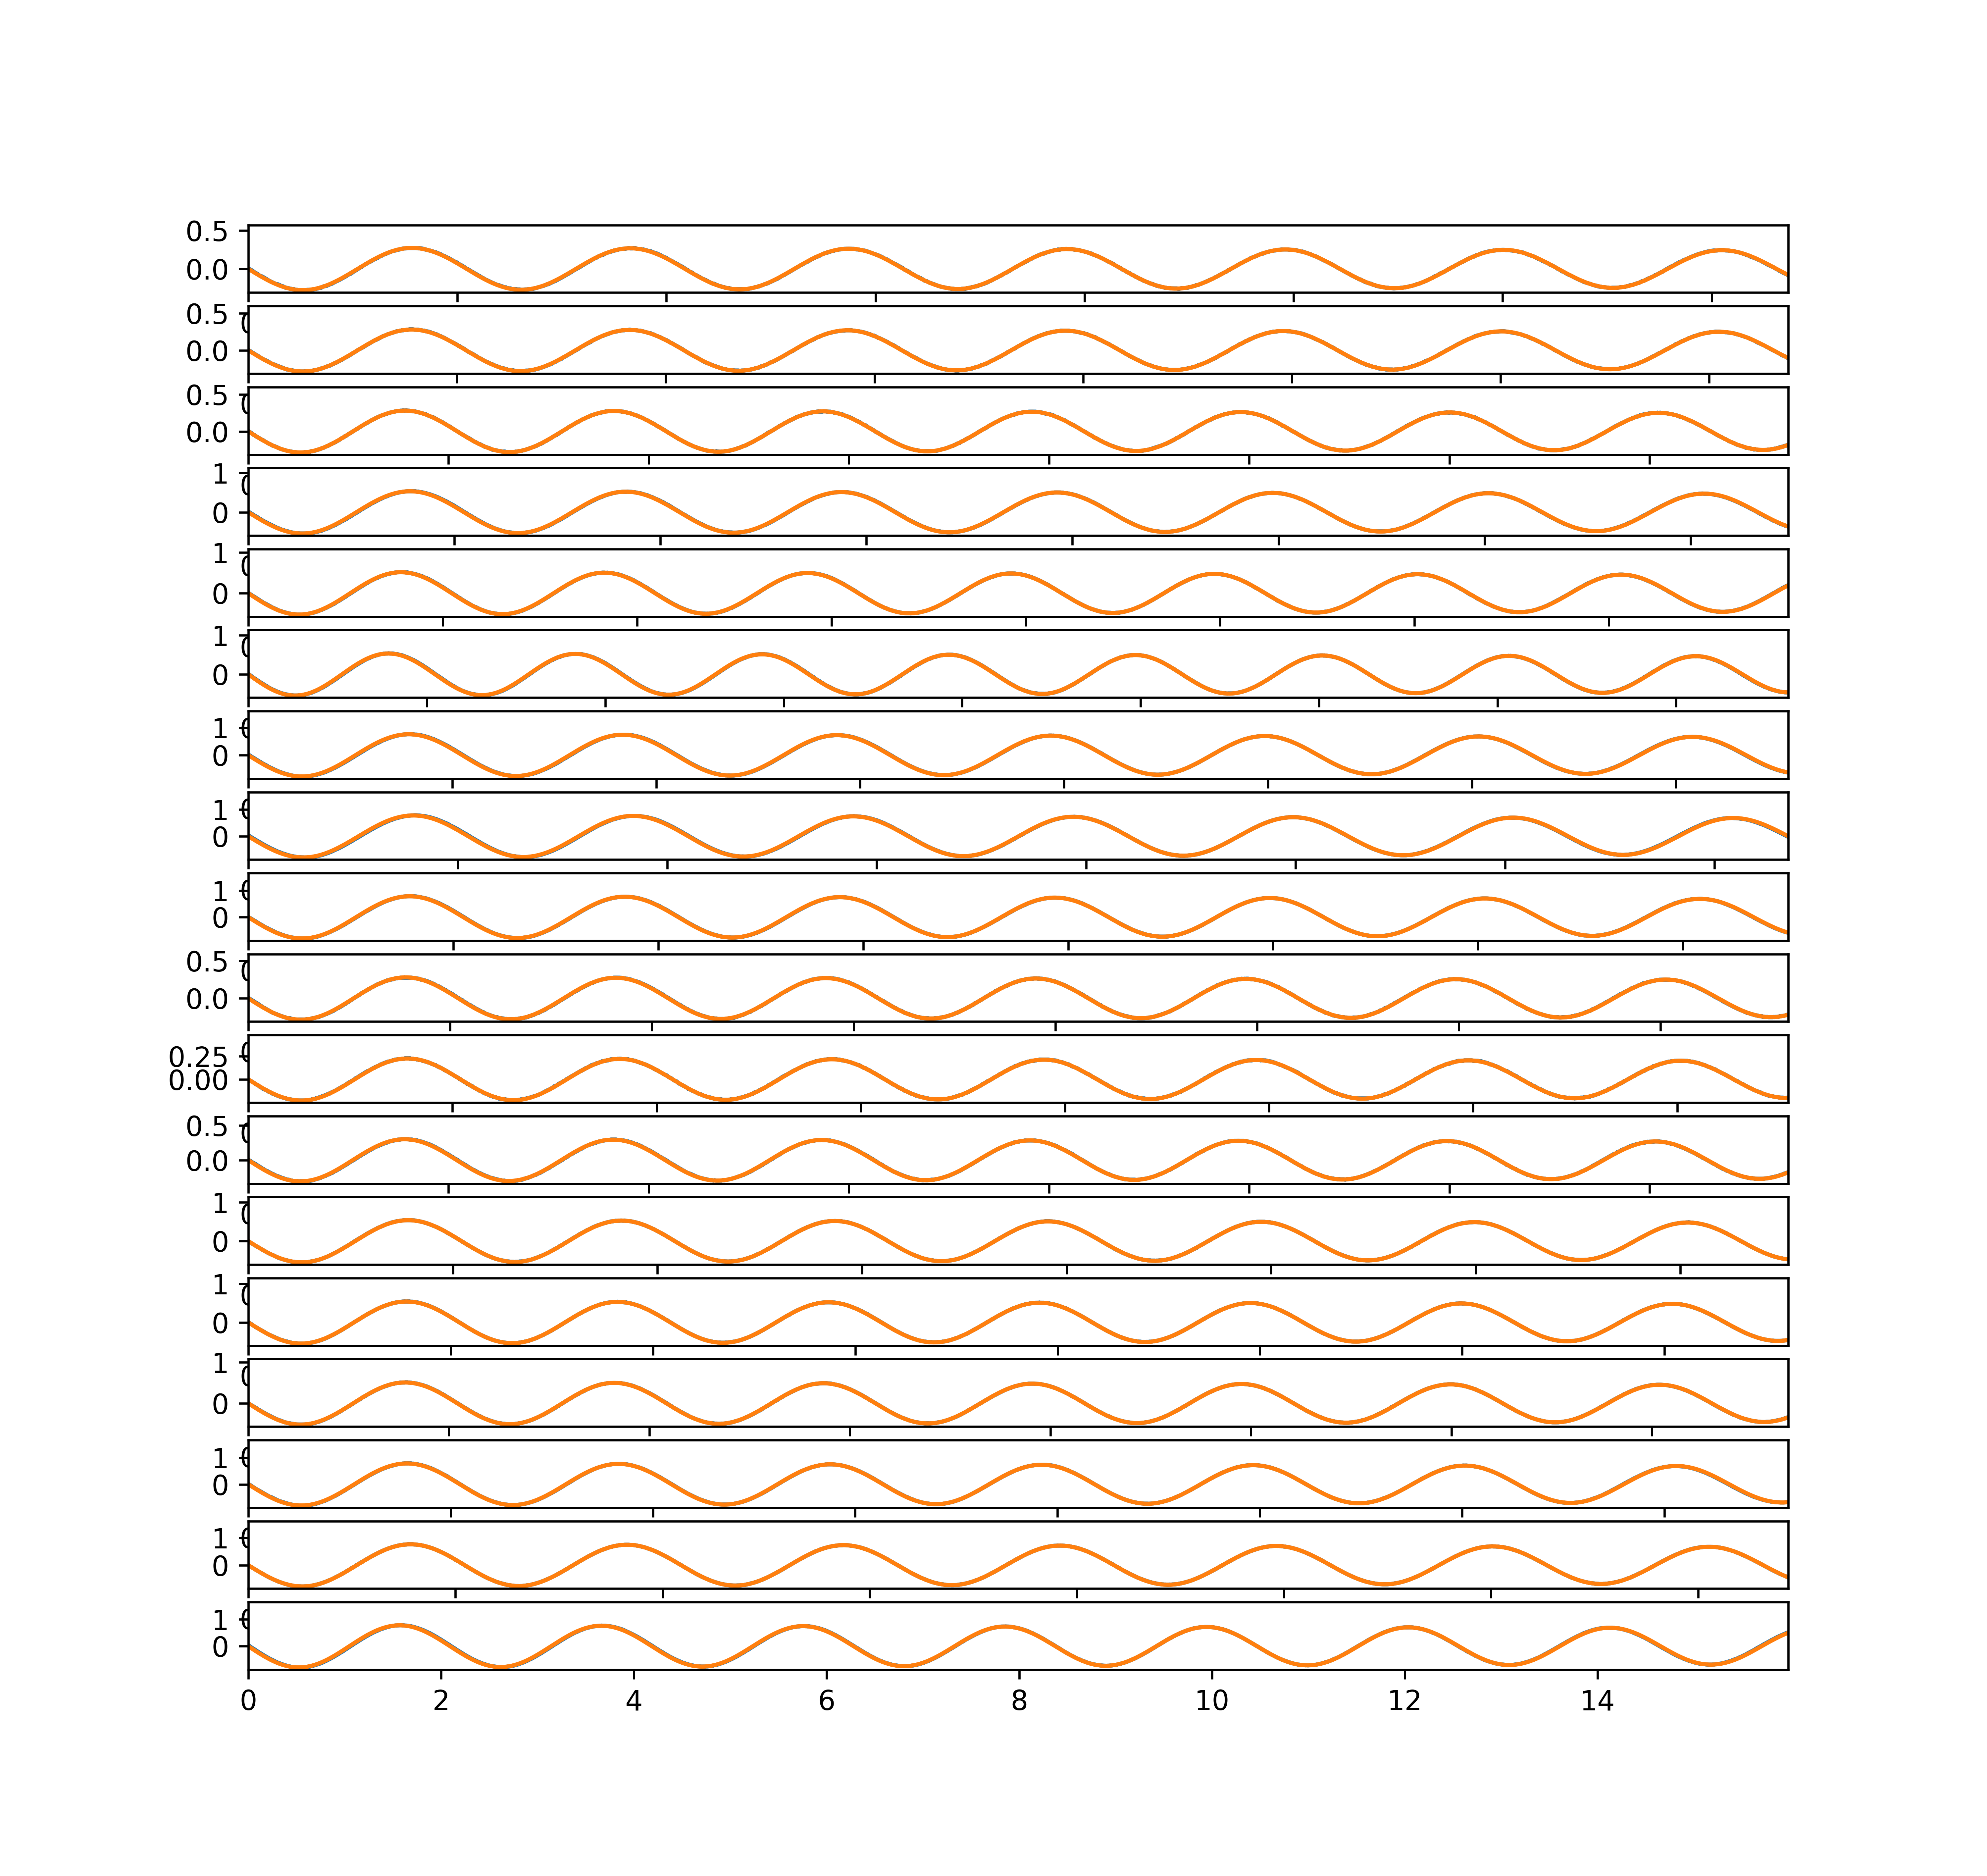
\includegraphics[width = 0.5\textwidth]{figure/damped_oscilation_fitdpi600.png}
    \caption{Fit of skateboard as compound pendulum}
    \label{f_dampedoscillation}
\end{figure}
The inertia results are given in figure \ref{f_inertianopower}
\begin{figure}
    \centering
    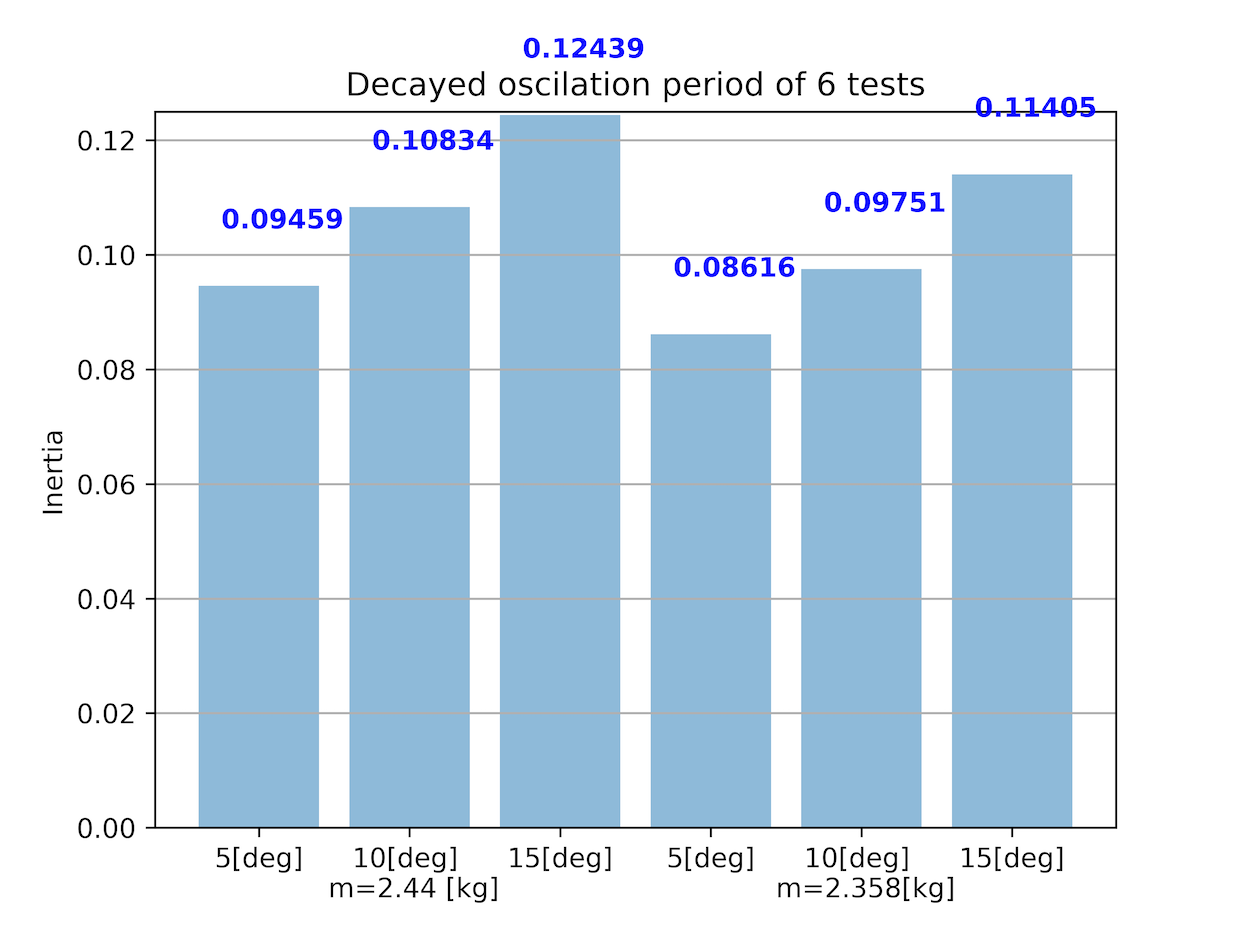
\includegraphics[width = 0.4\textwidth]{figure/Inertia_result_nopowerexpansiondpi600.png}
    \caption{Inertia results}
    \label{f_inertianopower}
\end{figure}
When it was clear that the inertia increased with an increase in starting angle, a power expansion is applied that accounts for small angle errors given by:
\begin{equation}
\begin{array}{r}
\omega_{exact} =  \approx T_0\left(1+\frac{1}{16} \theta^2+\frac{11}{3072} \theta^4+\frac{173}{737280} \theta^6\right. \\
\left.+\frac{22931}{1321205760} \theta^8+\ldots\right) .
\end{array}
\end{equation}
Which is used until the with precision $O^6$ results in the inertia data presented in figure \ref{f_powerexp}

\begin{figure}
    \centering
    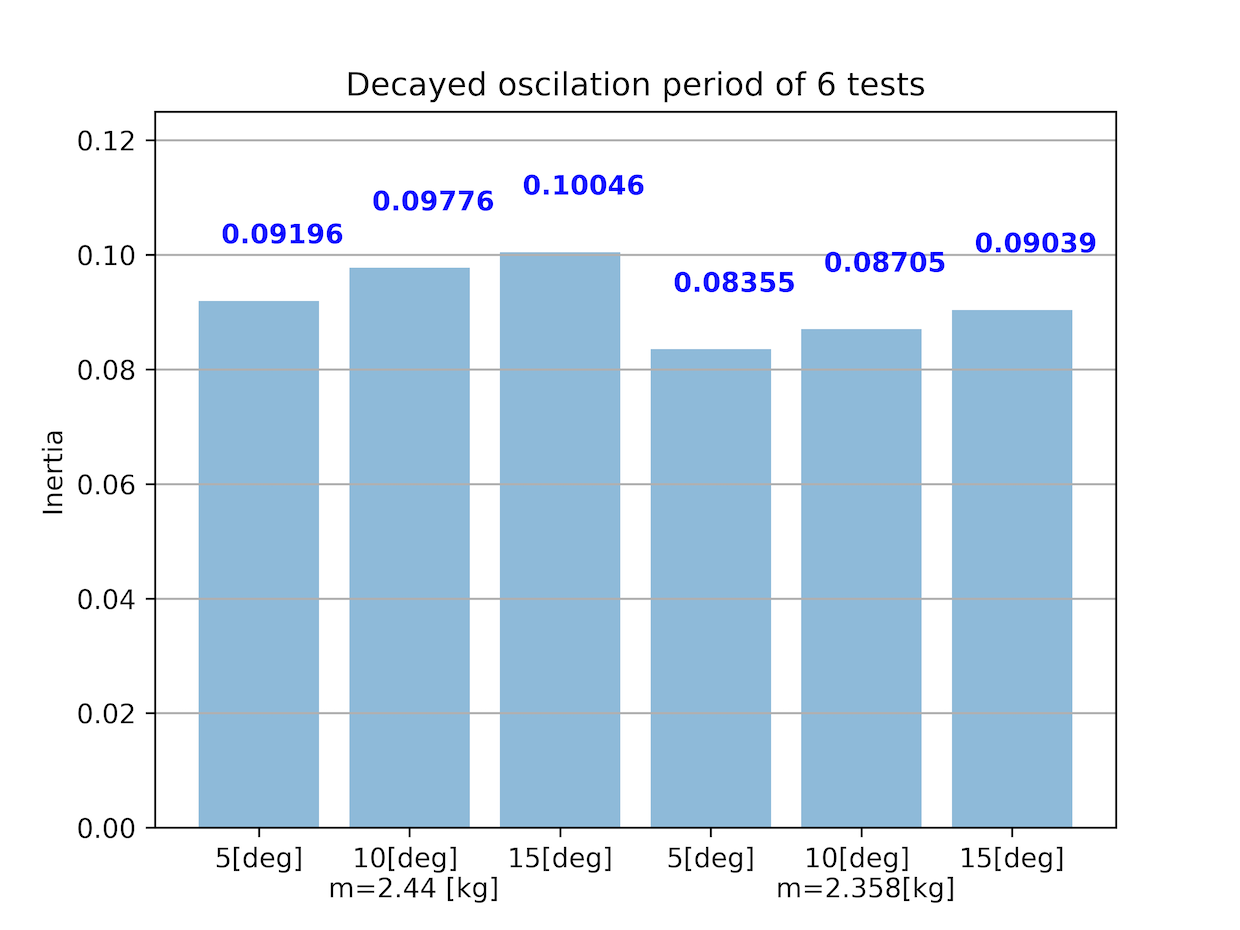
\includegraphics[width = 0.6\textwidth]{figure/Inertia_result_powerexpansiondpi600.png}
    \caption{Inertia result with power expansion}
    \label{f_powerexp}
\end{figure}

The calculated inertia value for skateboard with $m=2.44$ with the parameterized model is: 0.1219 [$kg\ m^2$]. The results show 0.09196 - 0.10046 [$kg\ m^2$]. The skateboards' inertia calculated with the parameterized model  with $m= 2.358$ is 0.1151 [$kg\ m^2$], while the results show 0.08355 - 0.09039 [$kg\ m^2$]. Both skateboards the model slightly overestimates the inertia.   The reduction in real life between the skateboards is 0.909\%, 0.890\%, 0.900\% between the different take off angles and different boards. In the parameterized model reduces inertia by 0.94 \%. This is of similar magnitude but needs more data to make it more exact. As a scaling approximation the parameter model is good enough.

\begin{figure}
    \centering
    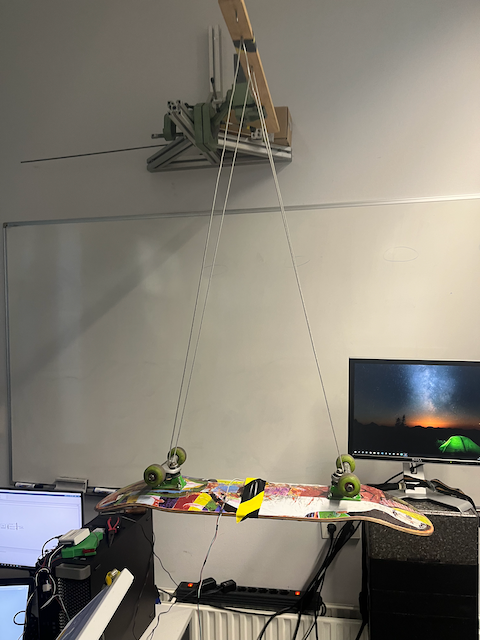
\includegraphics[width = 0.4 \textwidth]{figure/Testsetup.png}
    \caption{Test setup for inertia testing}
    \label{f_testsetup}
\end{figure}

\newpage
.
\newpage
\section*{Mass, centre of mass and inertia model}
\begin{verbatim}
    def Mass_model(width_deck, mass_bearing, mass_truck, height_truck, 
               height_truck0, width_wheel, n_ply, length_flat, length_tail, 
               radius_wheel, rho_pu, rho_maple, rho_steel, m_glue, 
               diameter_axle, d_veneer):

    mass_wheel = rho_pu * sm.pi * width_wheel * \
        ((2*radius_wheel)**2-diameter_axle**2) / 4  # V=pi*h*(D^2-d^2)/4

    mass_axle = sm.pi * (diameter_axle/2)**2 * width_deck * \
        rho_steel  # weight of axle, volume * steel * density

    #    _   _   ___________   _   _
    #  /  | | | |           | | | |  \
    # | 1 | |2| |     3     | |4| | 5 | 6=t1 7=w1 8=t2 9=w2
    #  \ _| |_| |___________| |_| |_ /

    #     1\                  /5
    #      2\_______3________/4
    #        6 \/         \/ 7
    #        8 O 9      10 O 11
    
    # Area of wooden components
    A1 = (1/2) * (1/4) * sm.pi * width_deck**2  # 1/4 pi d^2
    A2 = (length_tail - (width_deck/2)) * width_deck         # l * b
    A3 = length_flat * width_deck           # l * b
    A4 = A2
    A5 = A1
    
    thickness = n_ply*d_veneer
    dV = thickness*rho_maple+(m_glue/2*(n_ply-2))

    m1 = A1 * dV
    m2 = A2 * dV
    m3 = A3 * dV
    m4 = m2
    m5 = m1
    m6 = (mass_truck - mass_axle) * height_truck/height_truck0
    m7 = m6
    m8 = mass_axle
    m9 = 2*mass_wheel
    m10 = m8
    m11 = m9

    mass = [m1, m2, m3, m4, m5, m6, m7, m8, m9, m10, m11]
    return mass

def COM(mass, com_points, reference_point):
    # Function gets vector position from reference_point
    # Then assigns COM location to point COM
    # Returns position vector of COM points relative to COM
    r_m = []
    for i, x in enumerate(com_points):
        r_m.append(x.pos_from(reference_point)*mass[i])
    COM_skateboard = me.Point('COM_skateboard')
    COM_skateboard.set_pos(reference_point, (sum(r_m)/sum(mass)))
    return COM_skateboard
\end{verbatim}
\newpage
\begin{verbatim}
    
def Inertia_model(mass, com_points, com, majordim, shape):
    # Major dim:
    #   - (semi)cylinder;  diameter
    #   - cuboid: [l,h]
    #   - Triangle: [Base, Height]

    I_com = []
    I_steiner = []

    for i in range(len(mass)):
        if shape[i] == 'semicircle':
            I_com.append(((1/4)-(16/(9*sm.pi**2)))*mass[i]*(majordim[i]/2)**2)

        if shape[i] == 'cuboid':
            I_com.append((mass[i]/12) * (majordim[i]
                         [0]**2 + majordim[i][1]**2))

        if shape[i] == 'triangle':
            s = sm.sqrt((majordim[i][0]/2)**2+majordim[i][1]**2)
            beta = 2*sm.asin((majordim[i][0]/2)/s)
            I_com.append((mass[i]/2)*s**2*(1-(2/3)*sm.sin(beta)))

        if shape[i] == 'cylinder':
            I_com.append((1/2)*mass[i]*(majordim[i]/2)**2)
        #Trigsimp was sometimes necesarry due to a theta still being in there
        I_steiner.append(sm.trigsimp(mass[i]*d2s(sm.sqrt(com_points[i].\
        pos_from(com).dot(A.x)**2+com_points[i].pos_from(com).dot(A.y)**2)**2)))
    I_tot = sum(I_com)+sum(I_steiner)
    return I_tot, I_com, I_steiner
\end{verbatim}

\section*{Appendix B: Figures and tables}
\begin{table*}[h]
\begin{center}
\caption[Numerical bounds of state variables]{\centering Numerical bounds to state variables in the order of initial - absolute - final bounds. Final bound of $p^{(n)}$ equals initial bound of $p^{(n+1)}$. $v_{bound} = [-50,50]$} 
\begin{tabular}{r l l l l l l l l}\label{t_constraints}
& & \\ % put some space after the caption
\hline
ID         & Variable   & $p_0^{(1)}$ & $p^{(1)}_{bounds}$& $p_F^{(1)} = p_0^{2}$ & $p^{(2)}_{bounds}$ &$p_F^{(2)} = p_0^{(3)}$& $p^{(3)}_{bounds}$ &$p_F^{(3)}$  \\
\hline
\rownumber & $x_w$      & [-1, 0]     & [-2,1]            & [-2,1]               & -                  & -                   &  -                  & -\\
\rownumber & $x_s$      & -           & -                 &[-1,1]                & [-1,1]             & [-1, 1]             &  [-1,1]             & [-1,1]   \\
\rownumber & $y_s$      & -           & -                 &[0, 2]                & [0,5]              & [0, 5]              &  [0,5]              & [0,1] \\
\rownumber & $\theta_s$ & 0           & [0,$\pi$/2]       &[0, $\pi$/2 ]         & [-$\pi$/2 ,$\pi$/4]& 0                   & [$-\pi$/2, $\pi$/4] & [0, $\pi$/6]\\
\rownumber & $s_1$      & [0,1]       & [0,1]             &[0,1]                 & [0,1]              & [0,1]               & [0,1]              & [0,1]\\
\rownumber & $s_2 $     & [0,1]       & [0,1]             &[0,1]                 & [0,1]              & [0,1]               & [0,1]              & [0,1]\\
\rownumber & $x_h $     & 0           & [-1,1]            &[-1,1]                & [-1,1]             & [-1,1]              & [-1,1]             & [-1,1]\\
\rownumber & $y_h $     & [0,2]       & [0,5]             &[0,5]                 & [0,5]              & [0,5]               & [0,5]              & [0,5]\\
\rownumber & $\dot x_w$ & -           & $v_{bound}$       & $v_{bound}$          & -                  & -                   &  -                 &\\
\rownumber & $\dot x_s$ & 0           & $v_{bound}$       & $v_{bound}$          &$v_{bound}$         &$v_{bound}$          & $v_{bound}$        & $v_{bound}$  \\
\rownumber & $\dot y_s$ & 0           & $v_{bound}$       & $v_{bound}$          &$v_{bound}$         & 0                   &$v_{bound}$        & $v_{bound}$\\
\rownumber & $\dot \theta_s$ & 0      & $v_{bound}$       & $v_{bound}$          &$v_{bound}$         & $v_{bound}$         &$v_{bound}$        & $v_{bound}$ \\
\rownumber & $\dot s_1$ & 0           & $v_{bound}$       & $v_{bound}$          &$v_{bound}$         & $v_{bound}$         &$v_{bound}$        & $v_{bound}$ \\
\rownumber & $\dot s_2 $& 0           & $v_{bound}$       & $v_{bound}$          &$v_{bound}$         & $v_{bound}$         &$v_{bound}$        & $v_{bound}$ \\
\rownumber & $\dot x_h $& 0           & $v_{bound}$       & $v_{bound}$          &$v_{bound}$         & $v_{bound}$         &$v_{bound}$        & $v_{bound}$ \\
\rownumber & $\dot y_h $& 0           & $v_{bound}$       & $v_{bound}$          &$v_{bound}$         & $v_{bound}$         &$v_{bound}$        & $v_{bound}$ \\

\hline
\end{tabular}
\end{center}
\end{table*}
\section*{Results of optimal board shapes}
Detailed trajectories, states and control of all optimizations shown in figures \ref{f_nopar}, \ref{f_singlepar}, and \ref{f_multipar}
\begin{figure*}[b]
    \subfloat[Long board]{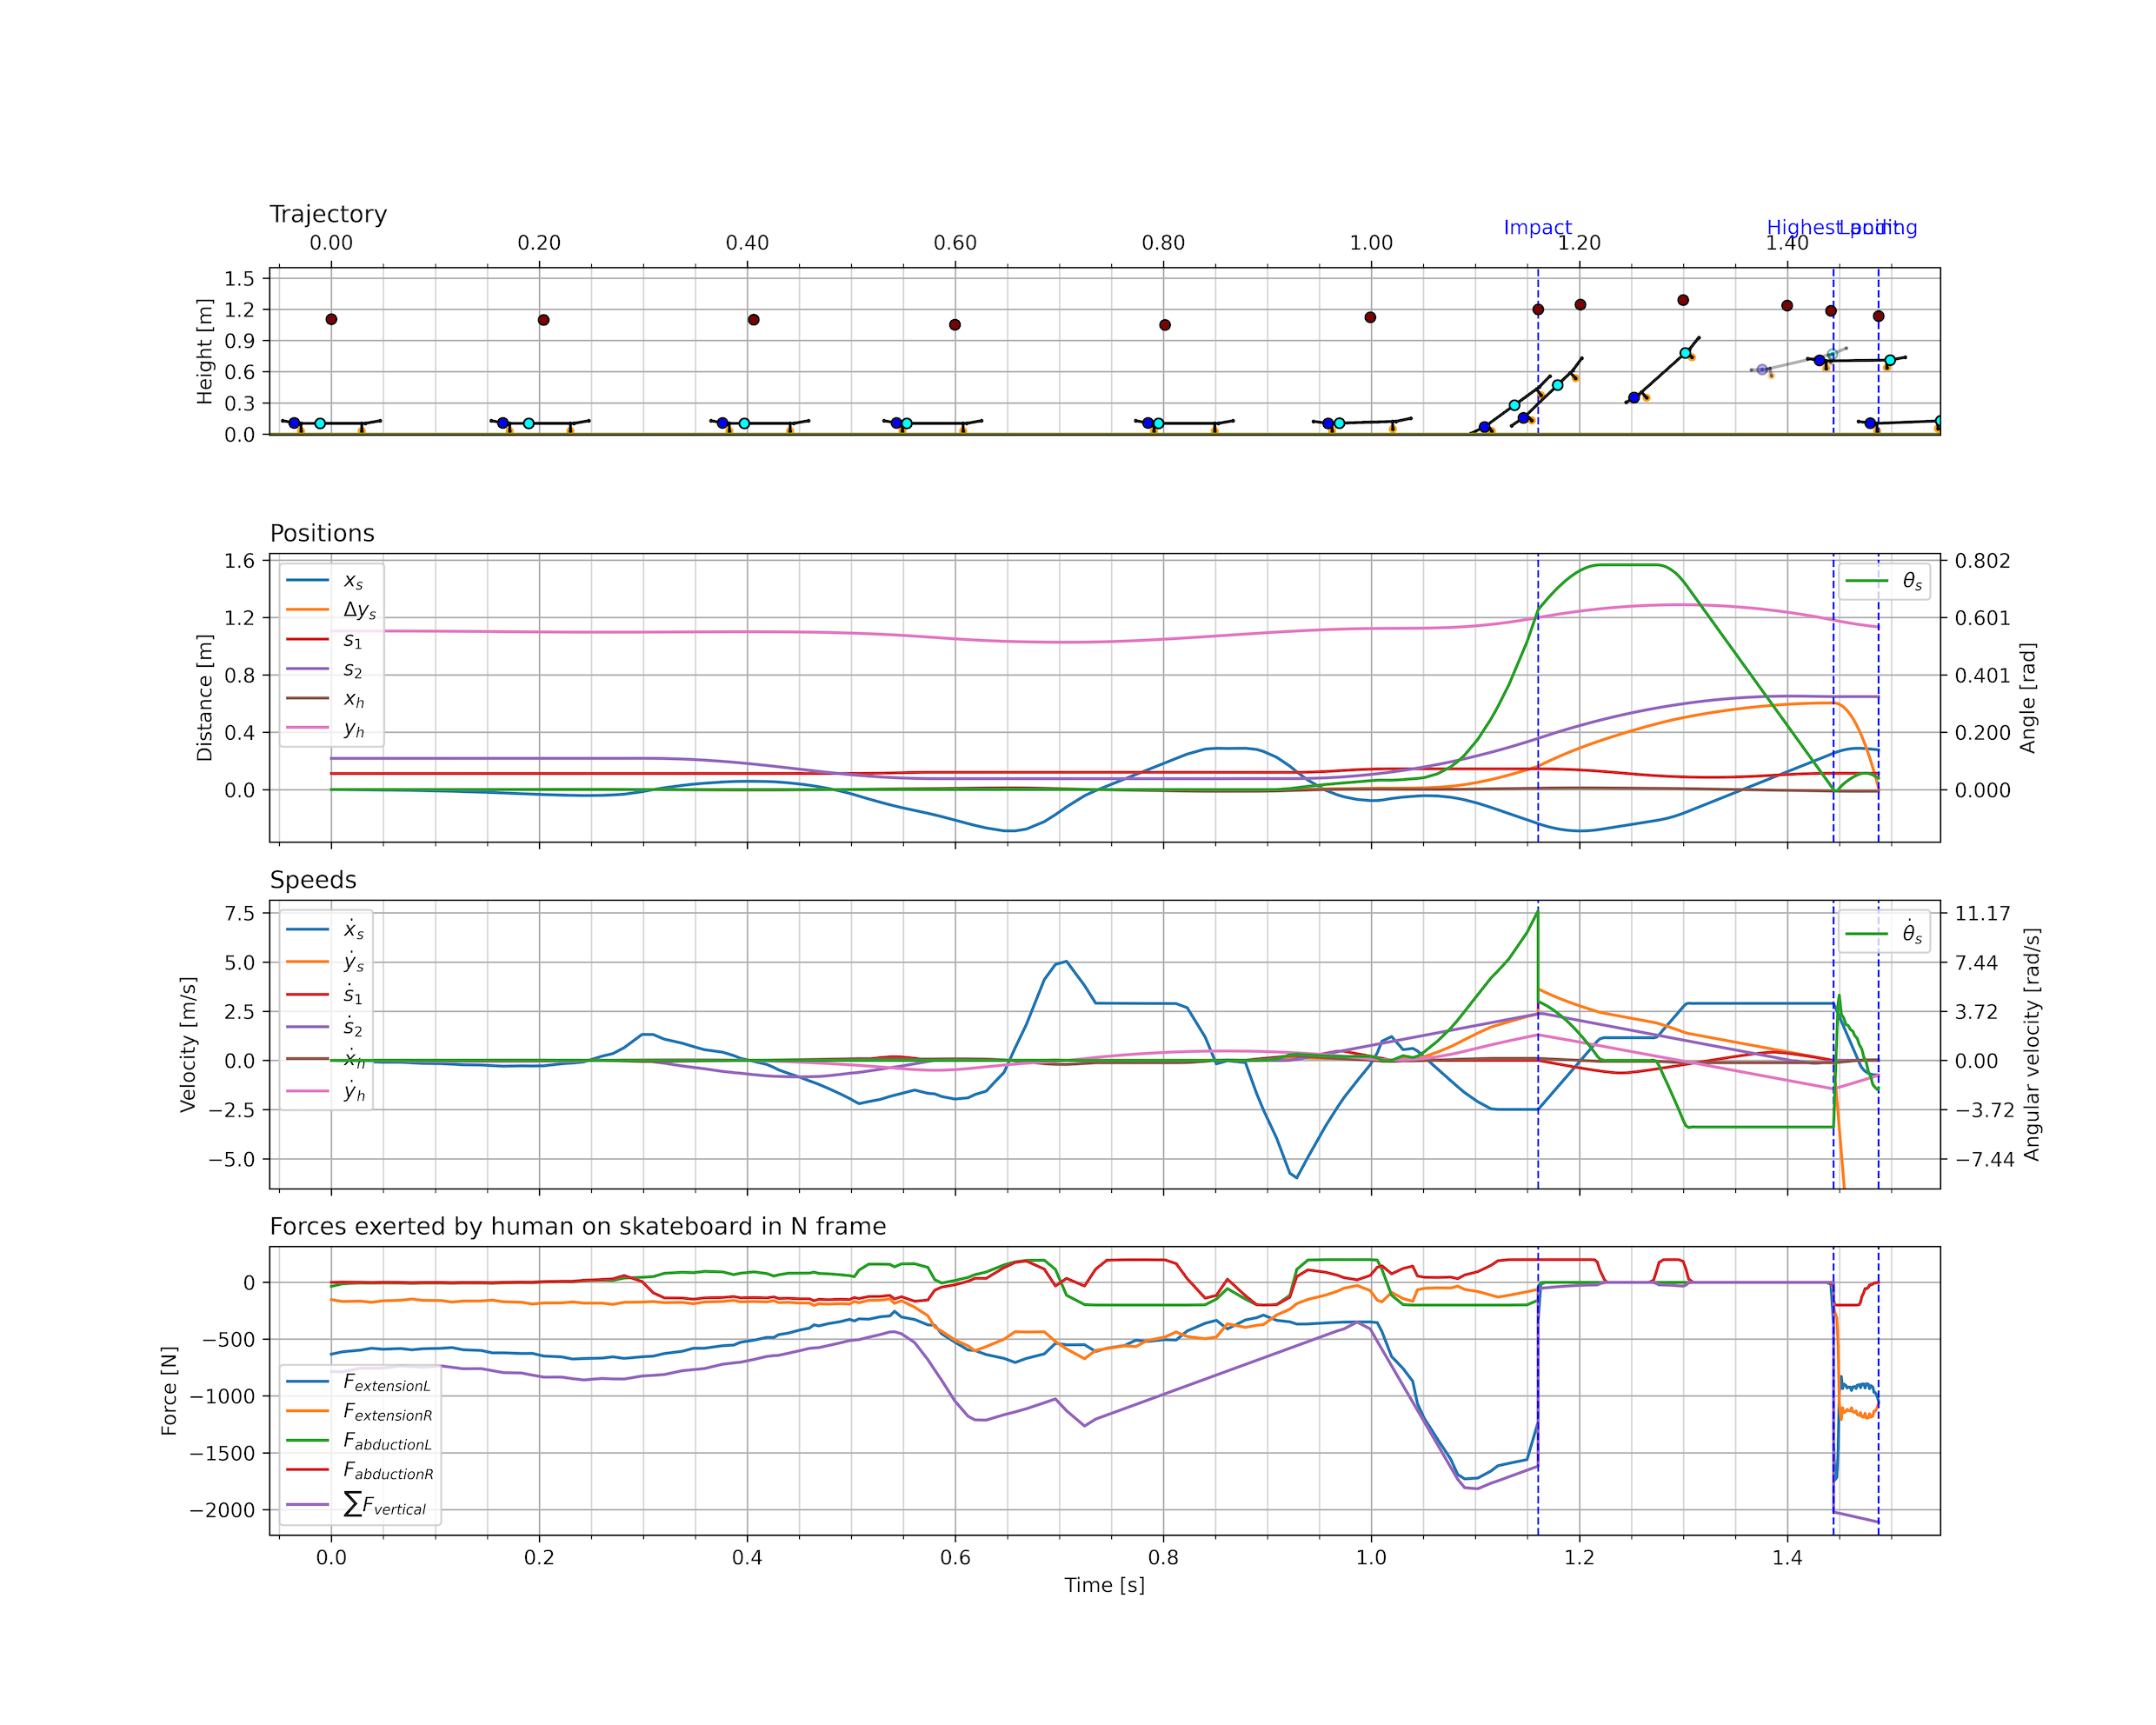
\includegraphics[trim={0cm 0cm 0cm 0cm},clip,width=0.8\textwidth]{figure/Results/data_longboard_init_longer_tail_optdpi600.png}}
    \newline
    \subfloat[All parameters no trucks]{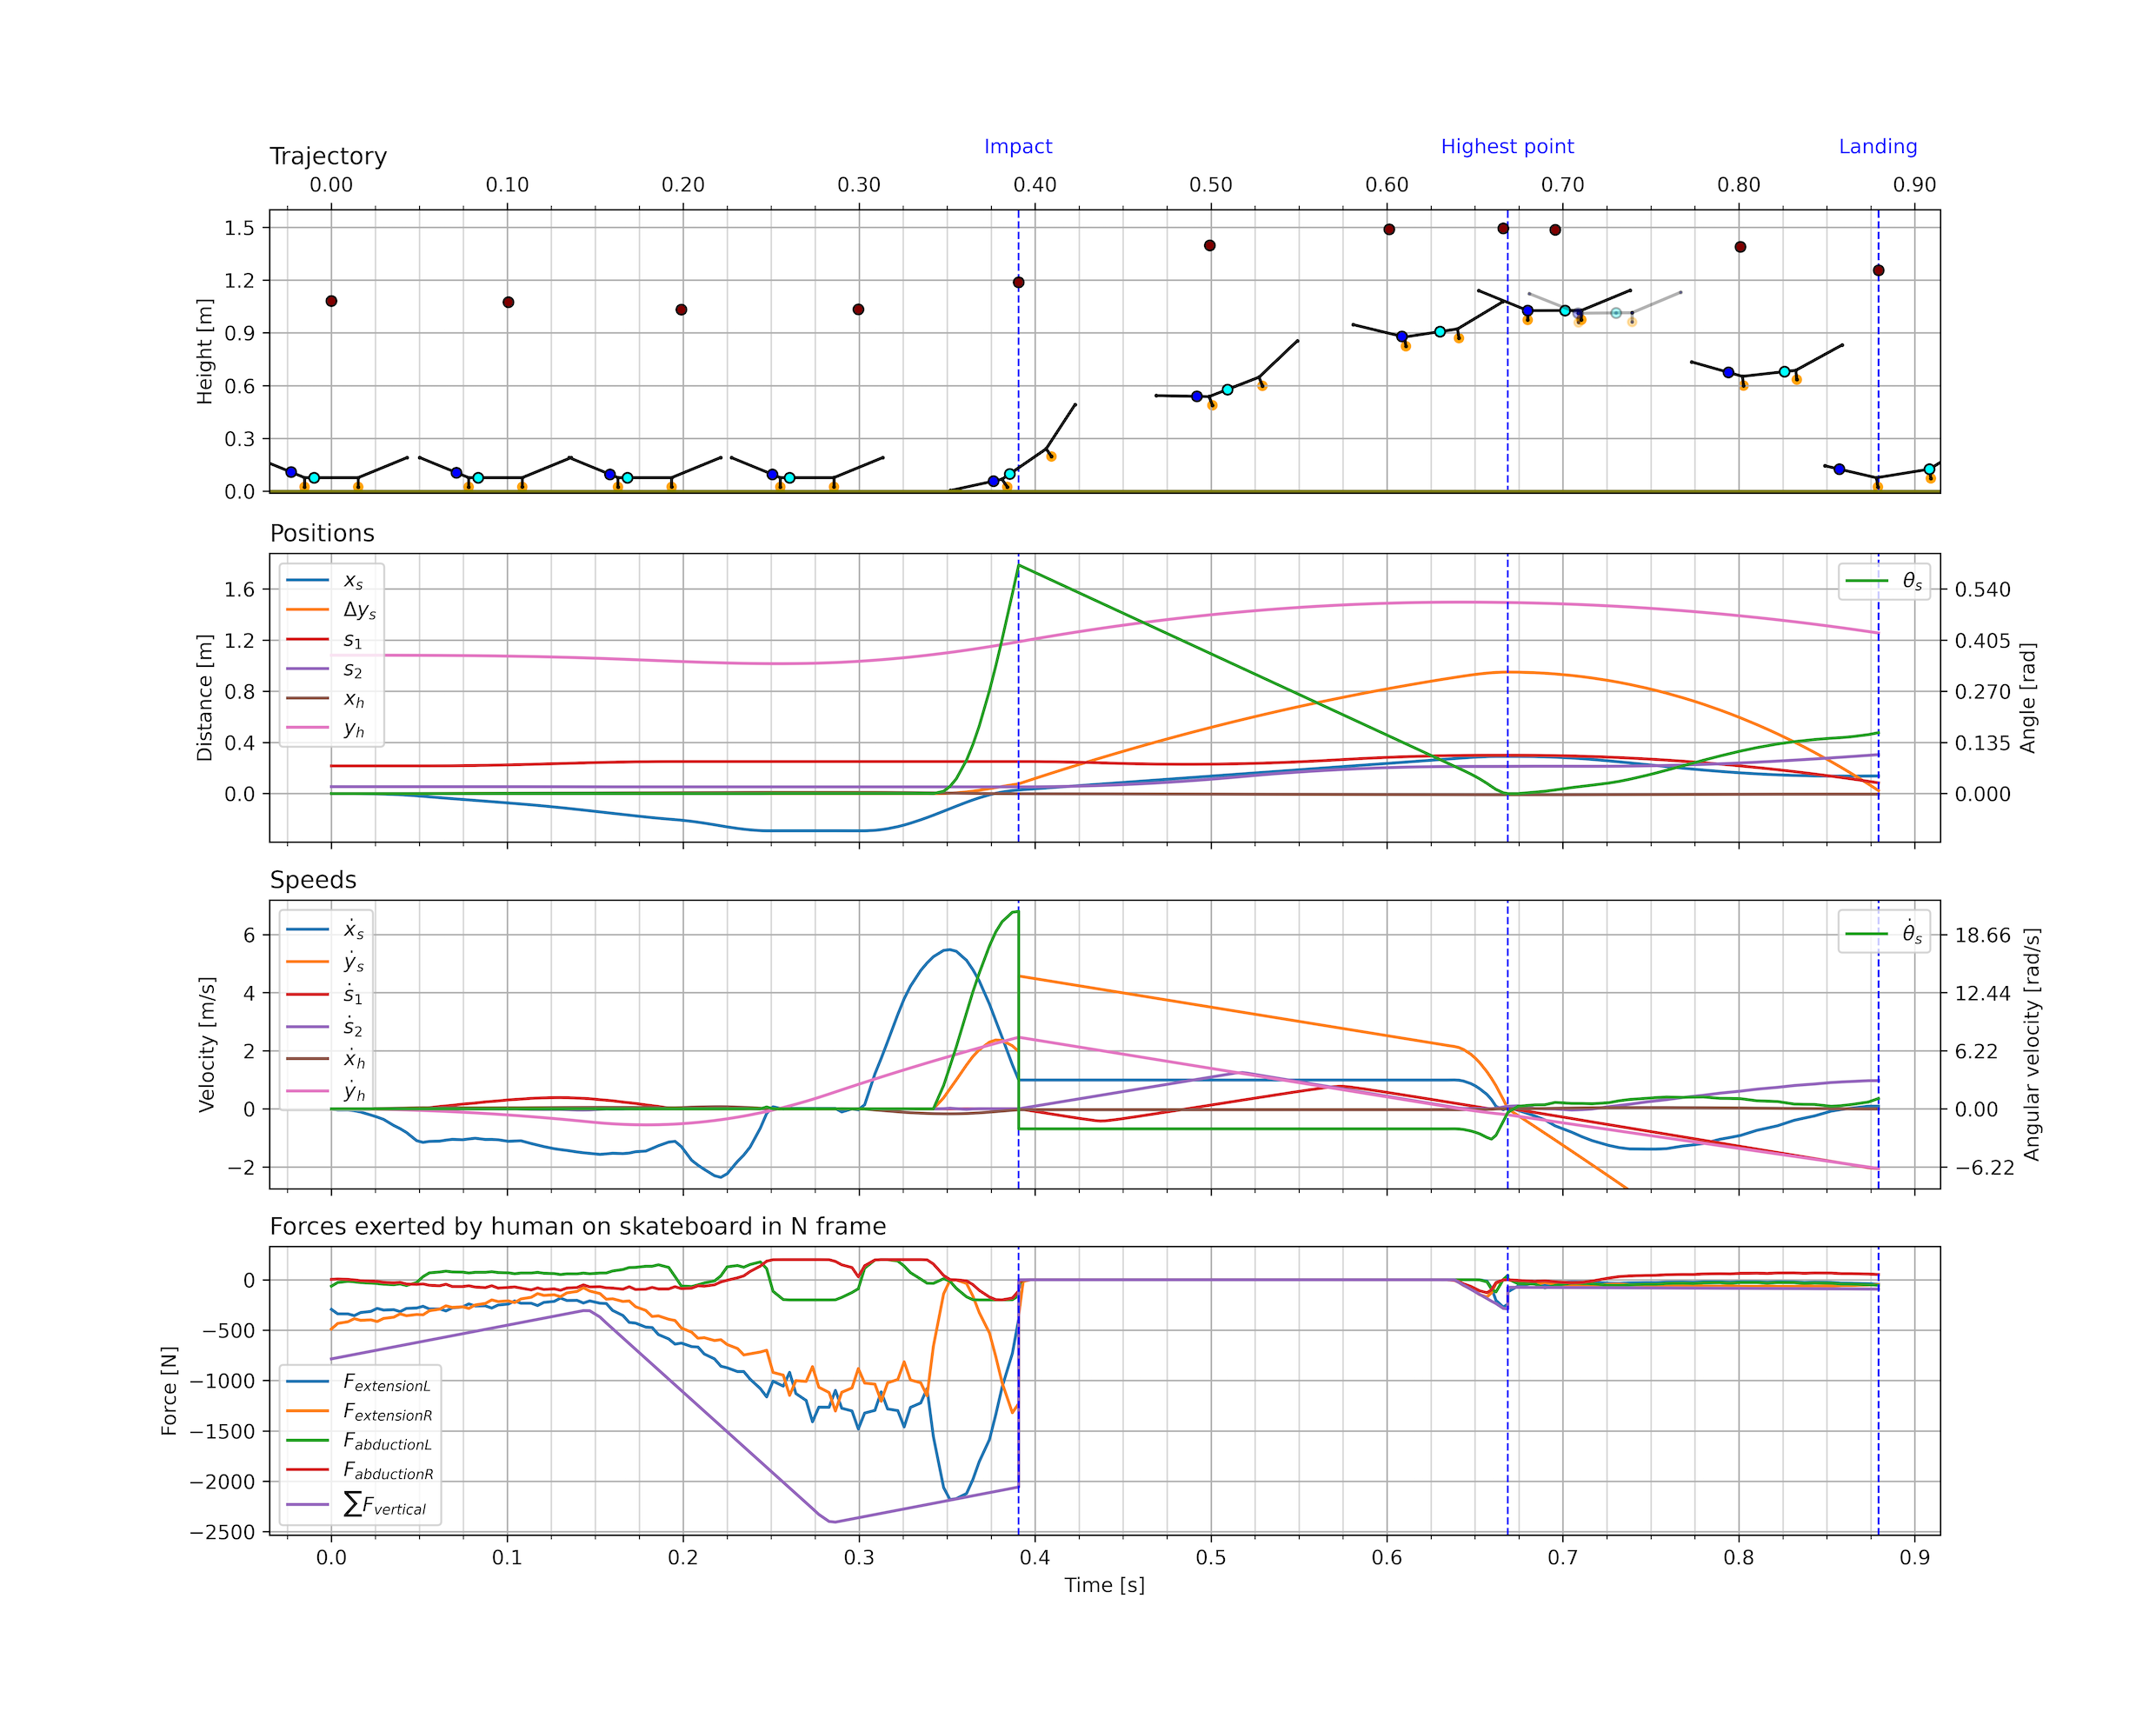
\includegraphics[trim={0cm 0cm 0cm 0cm},clip,width=0.8\textwidth]{figure/Results/data_notrrwdpi600.png}}
    \label{f_longboard}
    \caption{Longboard and `all except trucks' optimization results}
\end{figure*}

\begin{figure*}[b]    
    \subfloat[Plastic]{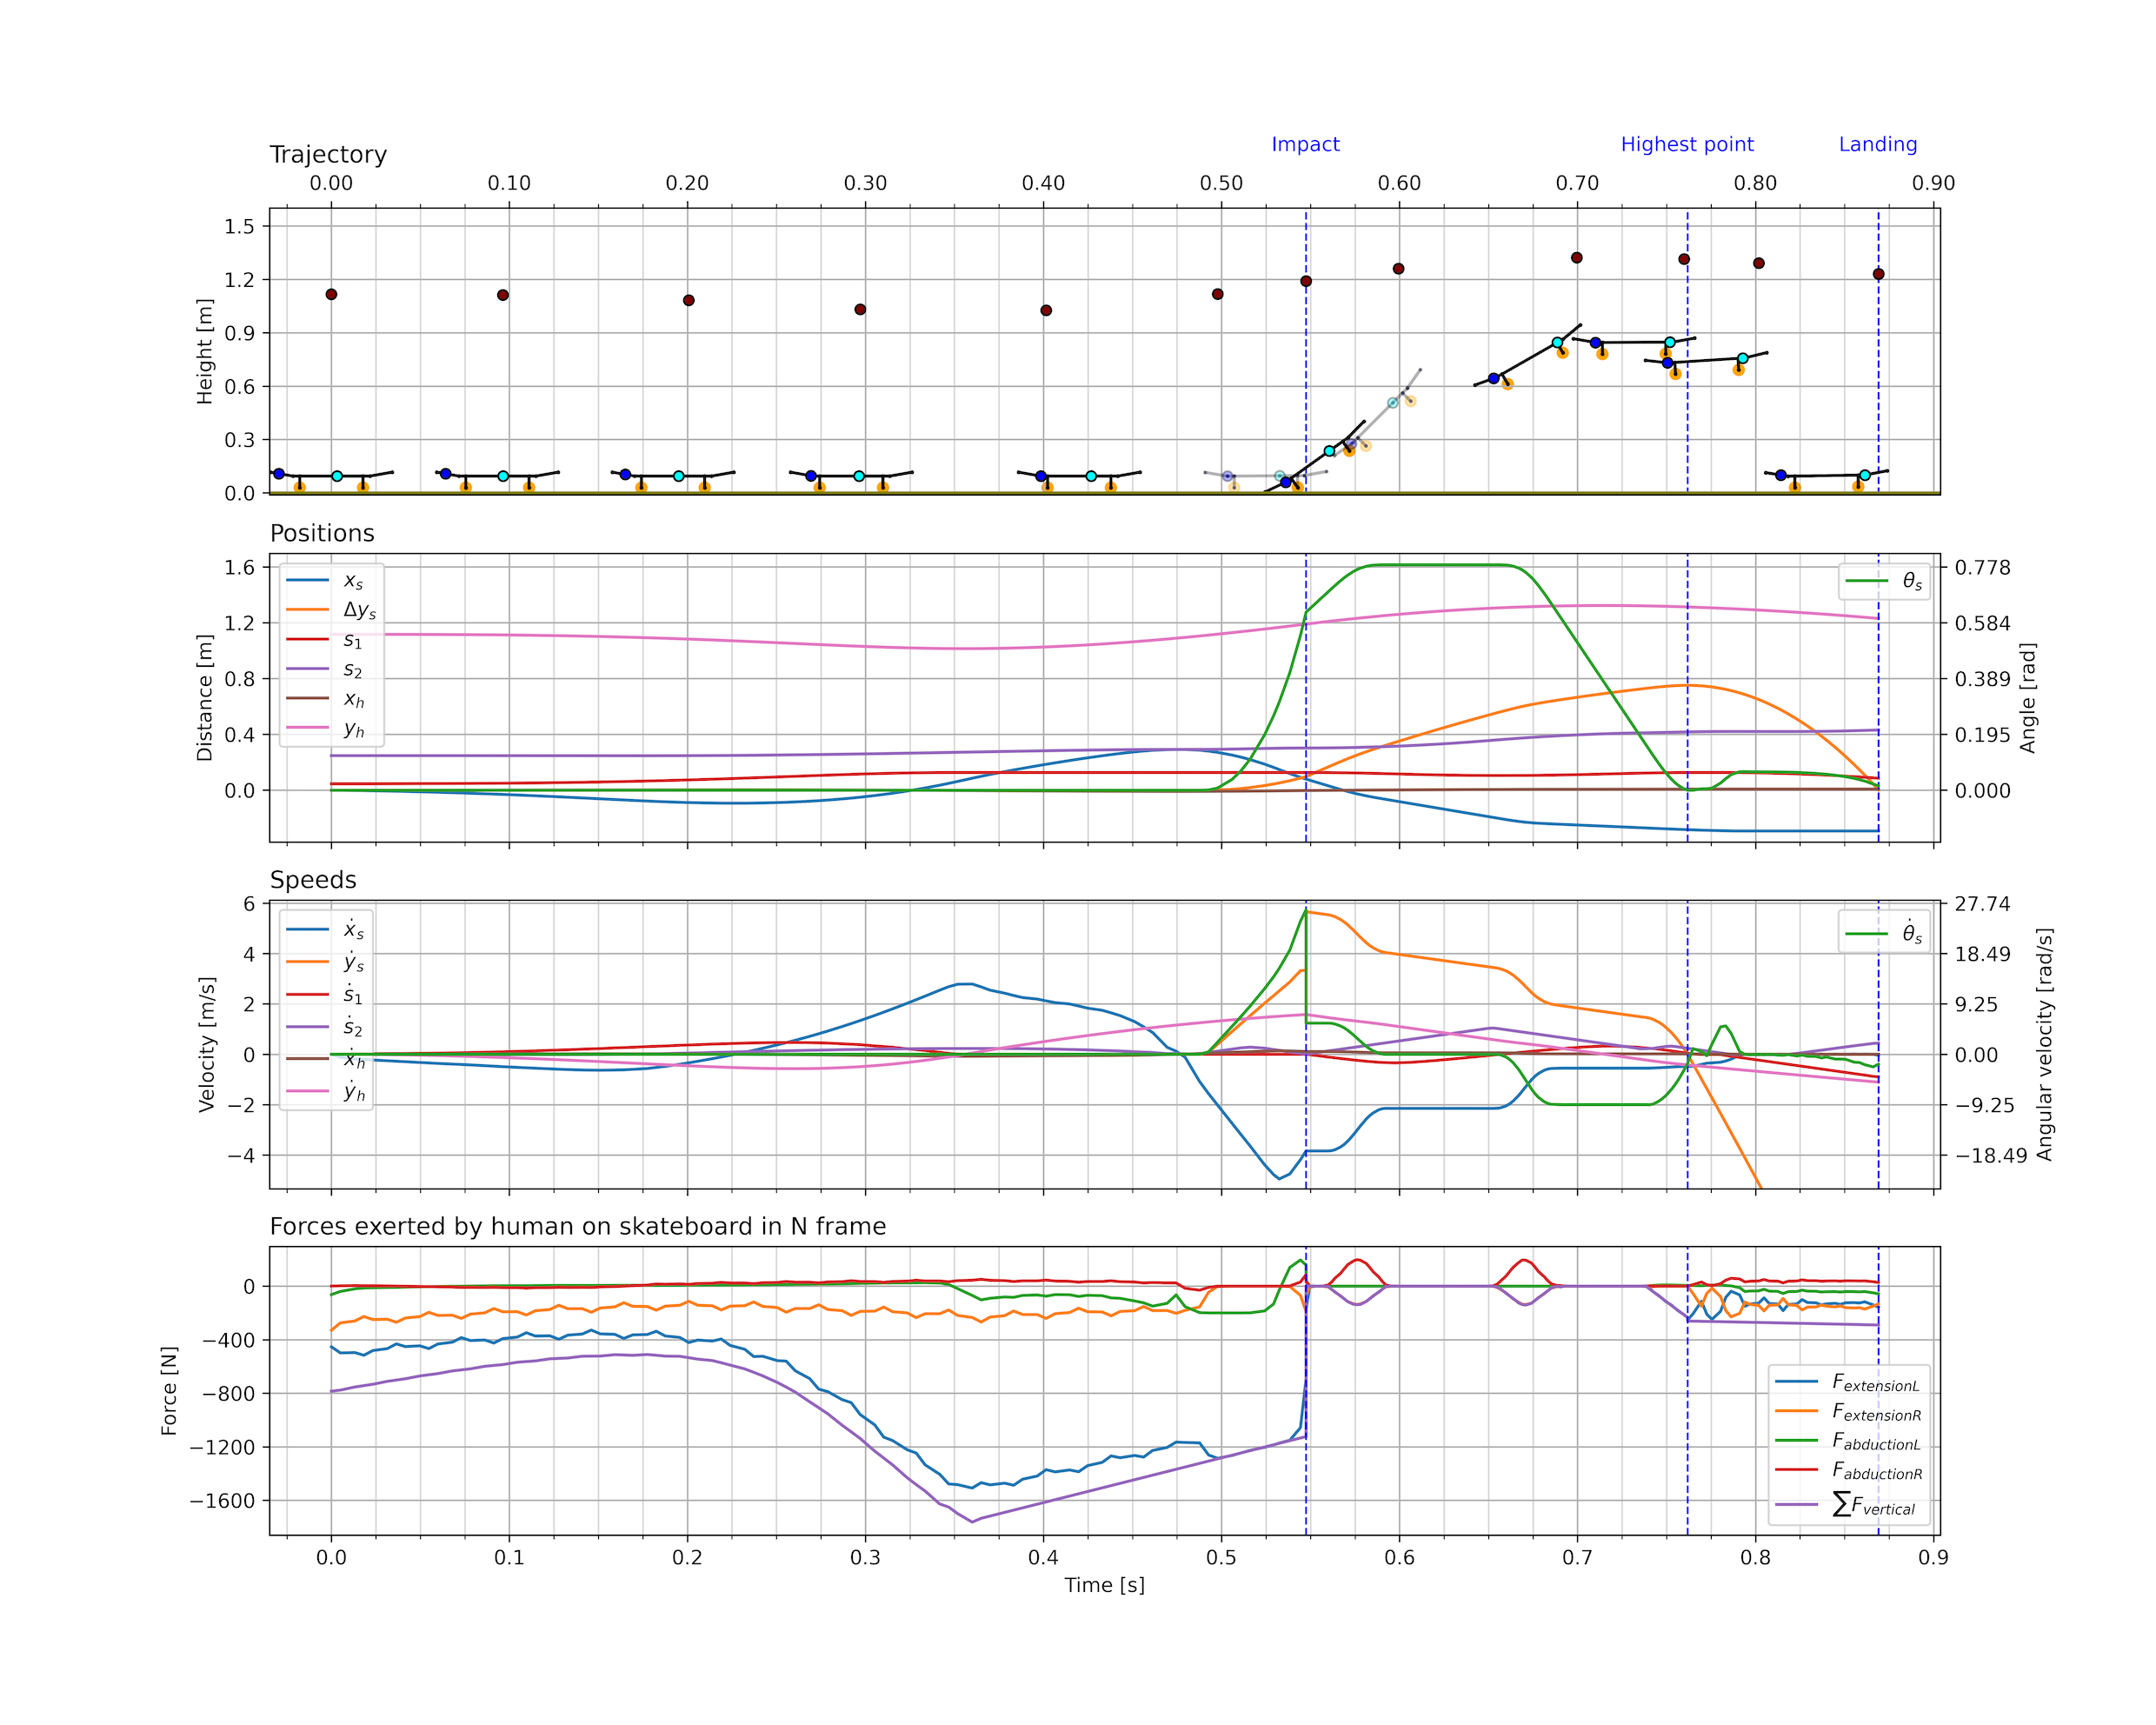
\includegraphics[trim={0cm 0cm 0cm 0cm},clip,width=0.8\textwidth]{figure/Results/data_penny_02dpi600.png}}
    \newline
    \subfloat[Griptape]{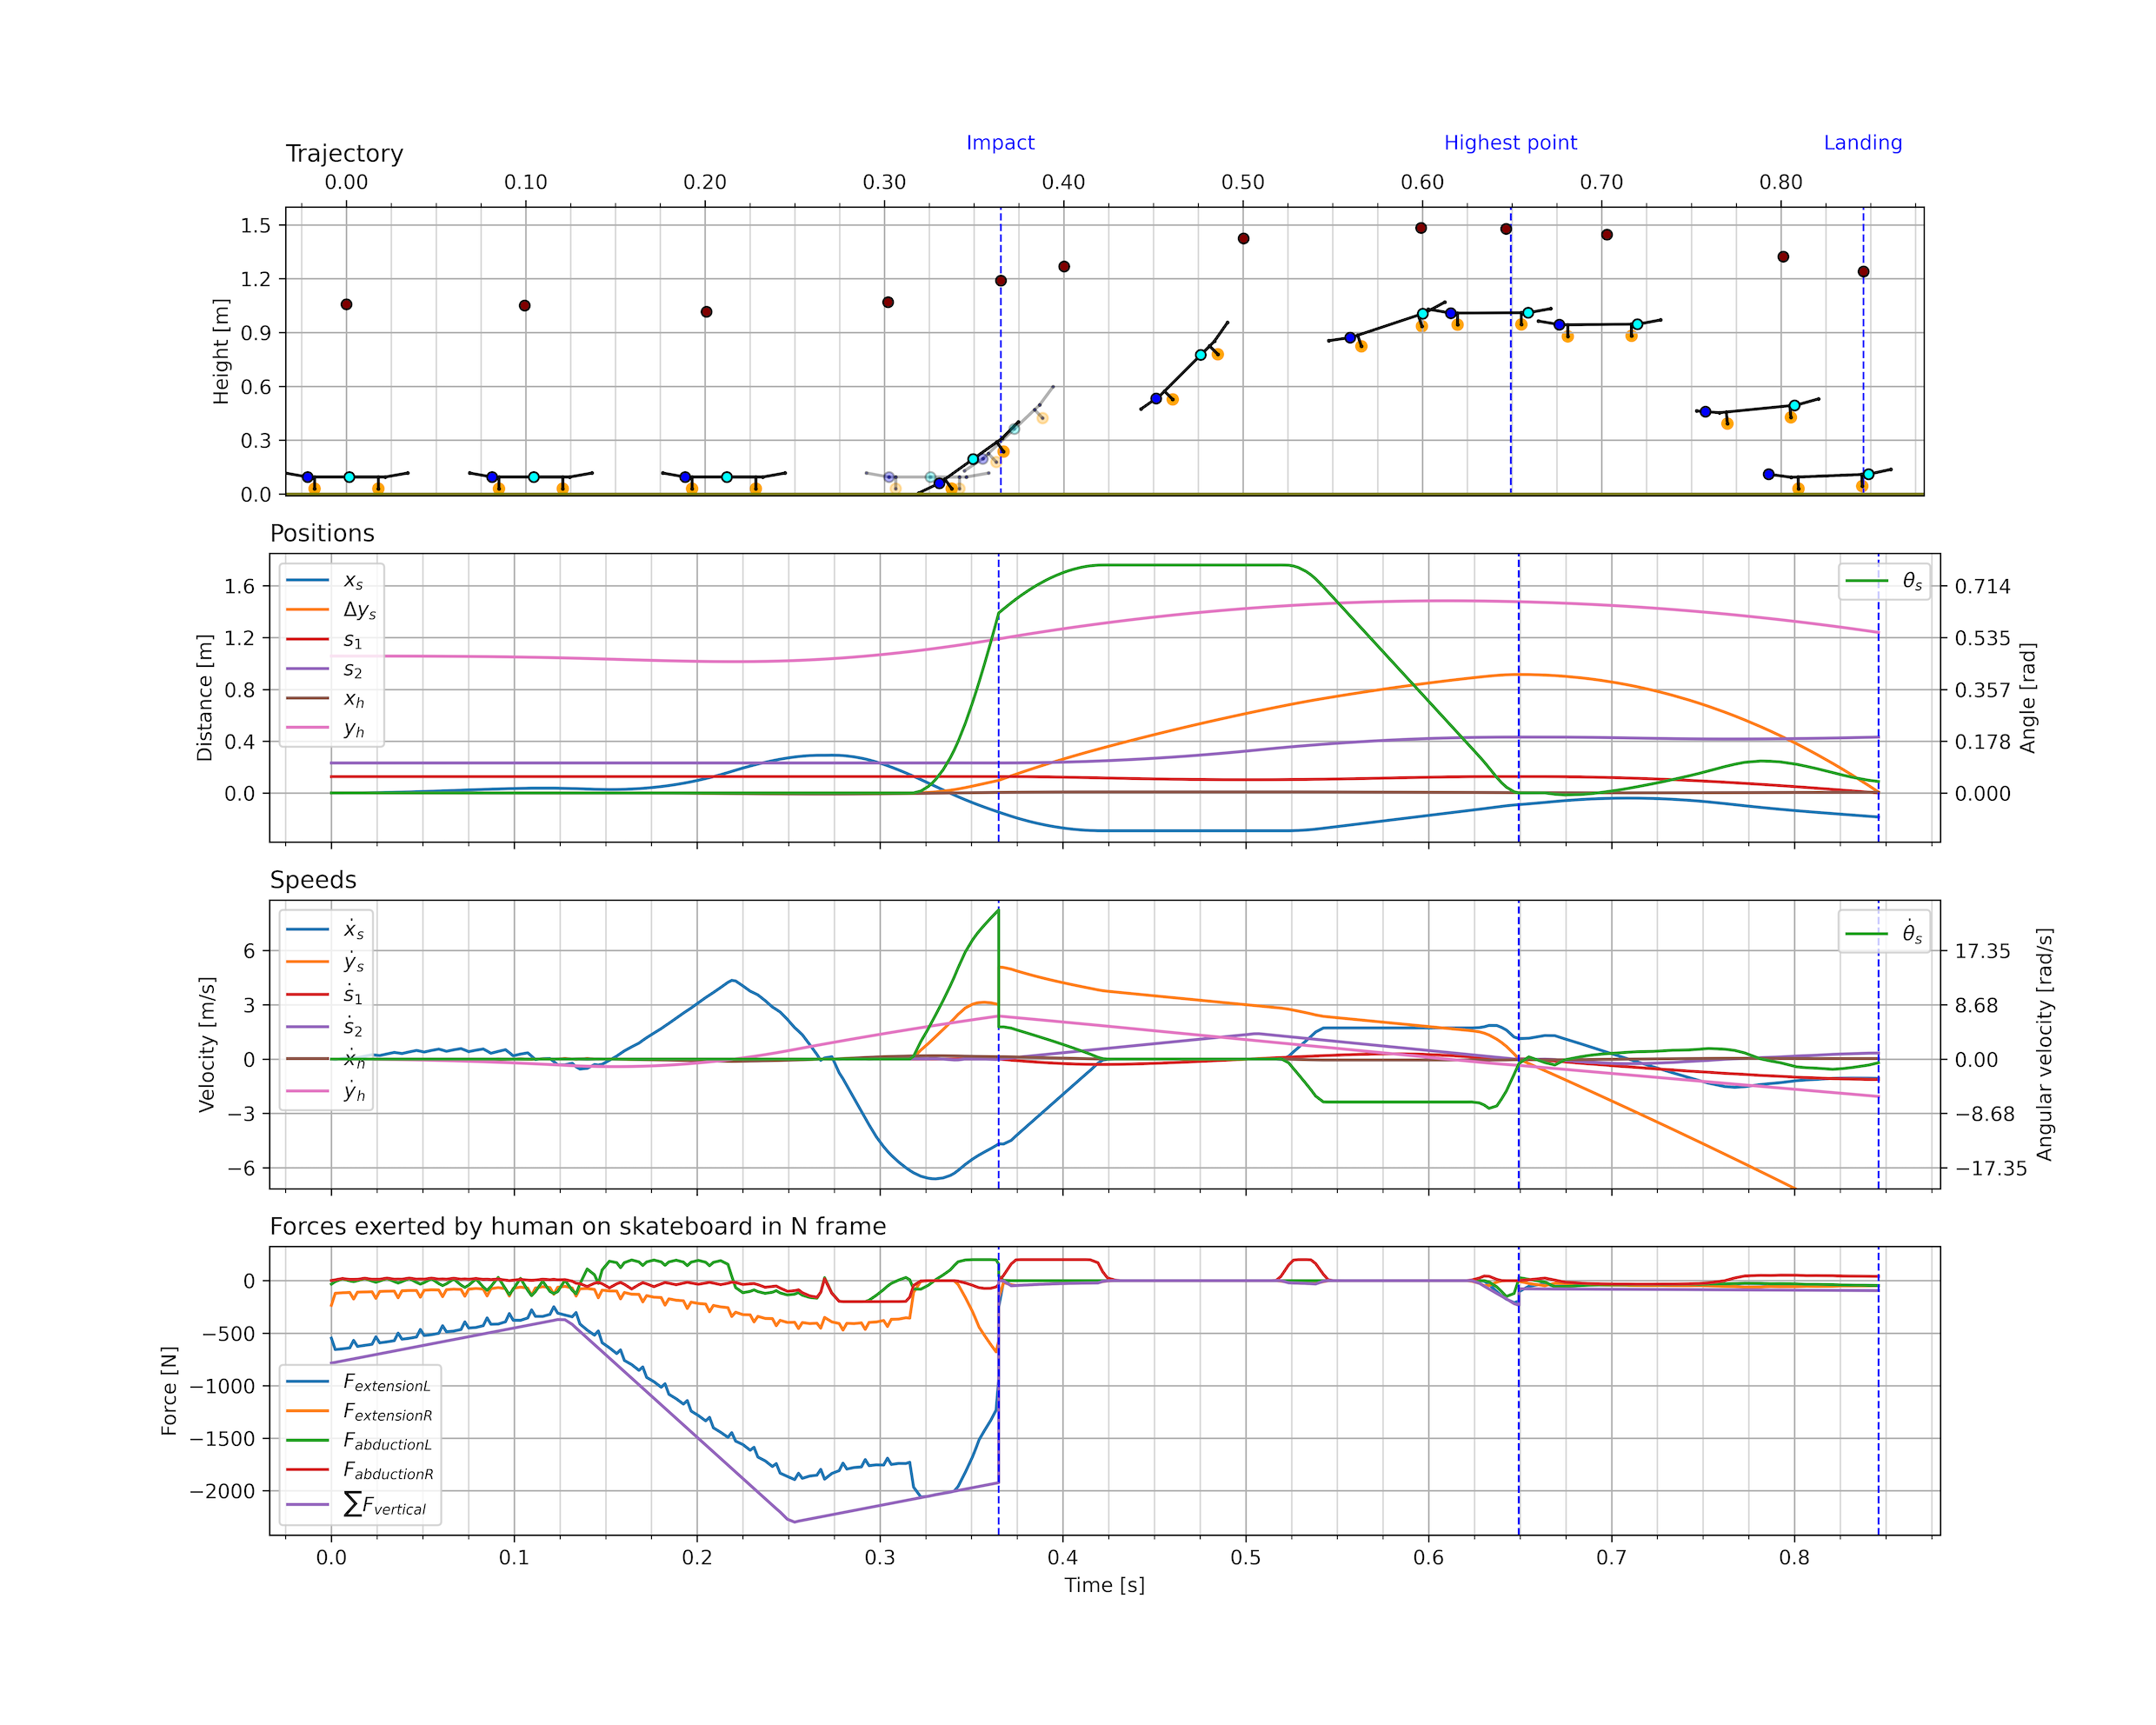
\includegraphics[trim={0cm 0cm 0cm 0cm},clip,width=0.8\textwidth]{figure/Results/data_penny_08dpi600.png}}
    \caption{Penny boards optimization results}    
\end{figure*}

\begin{figure*}[b]    
    \subfloat[Wheel radius]{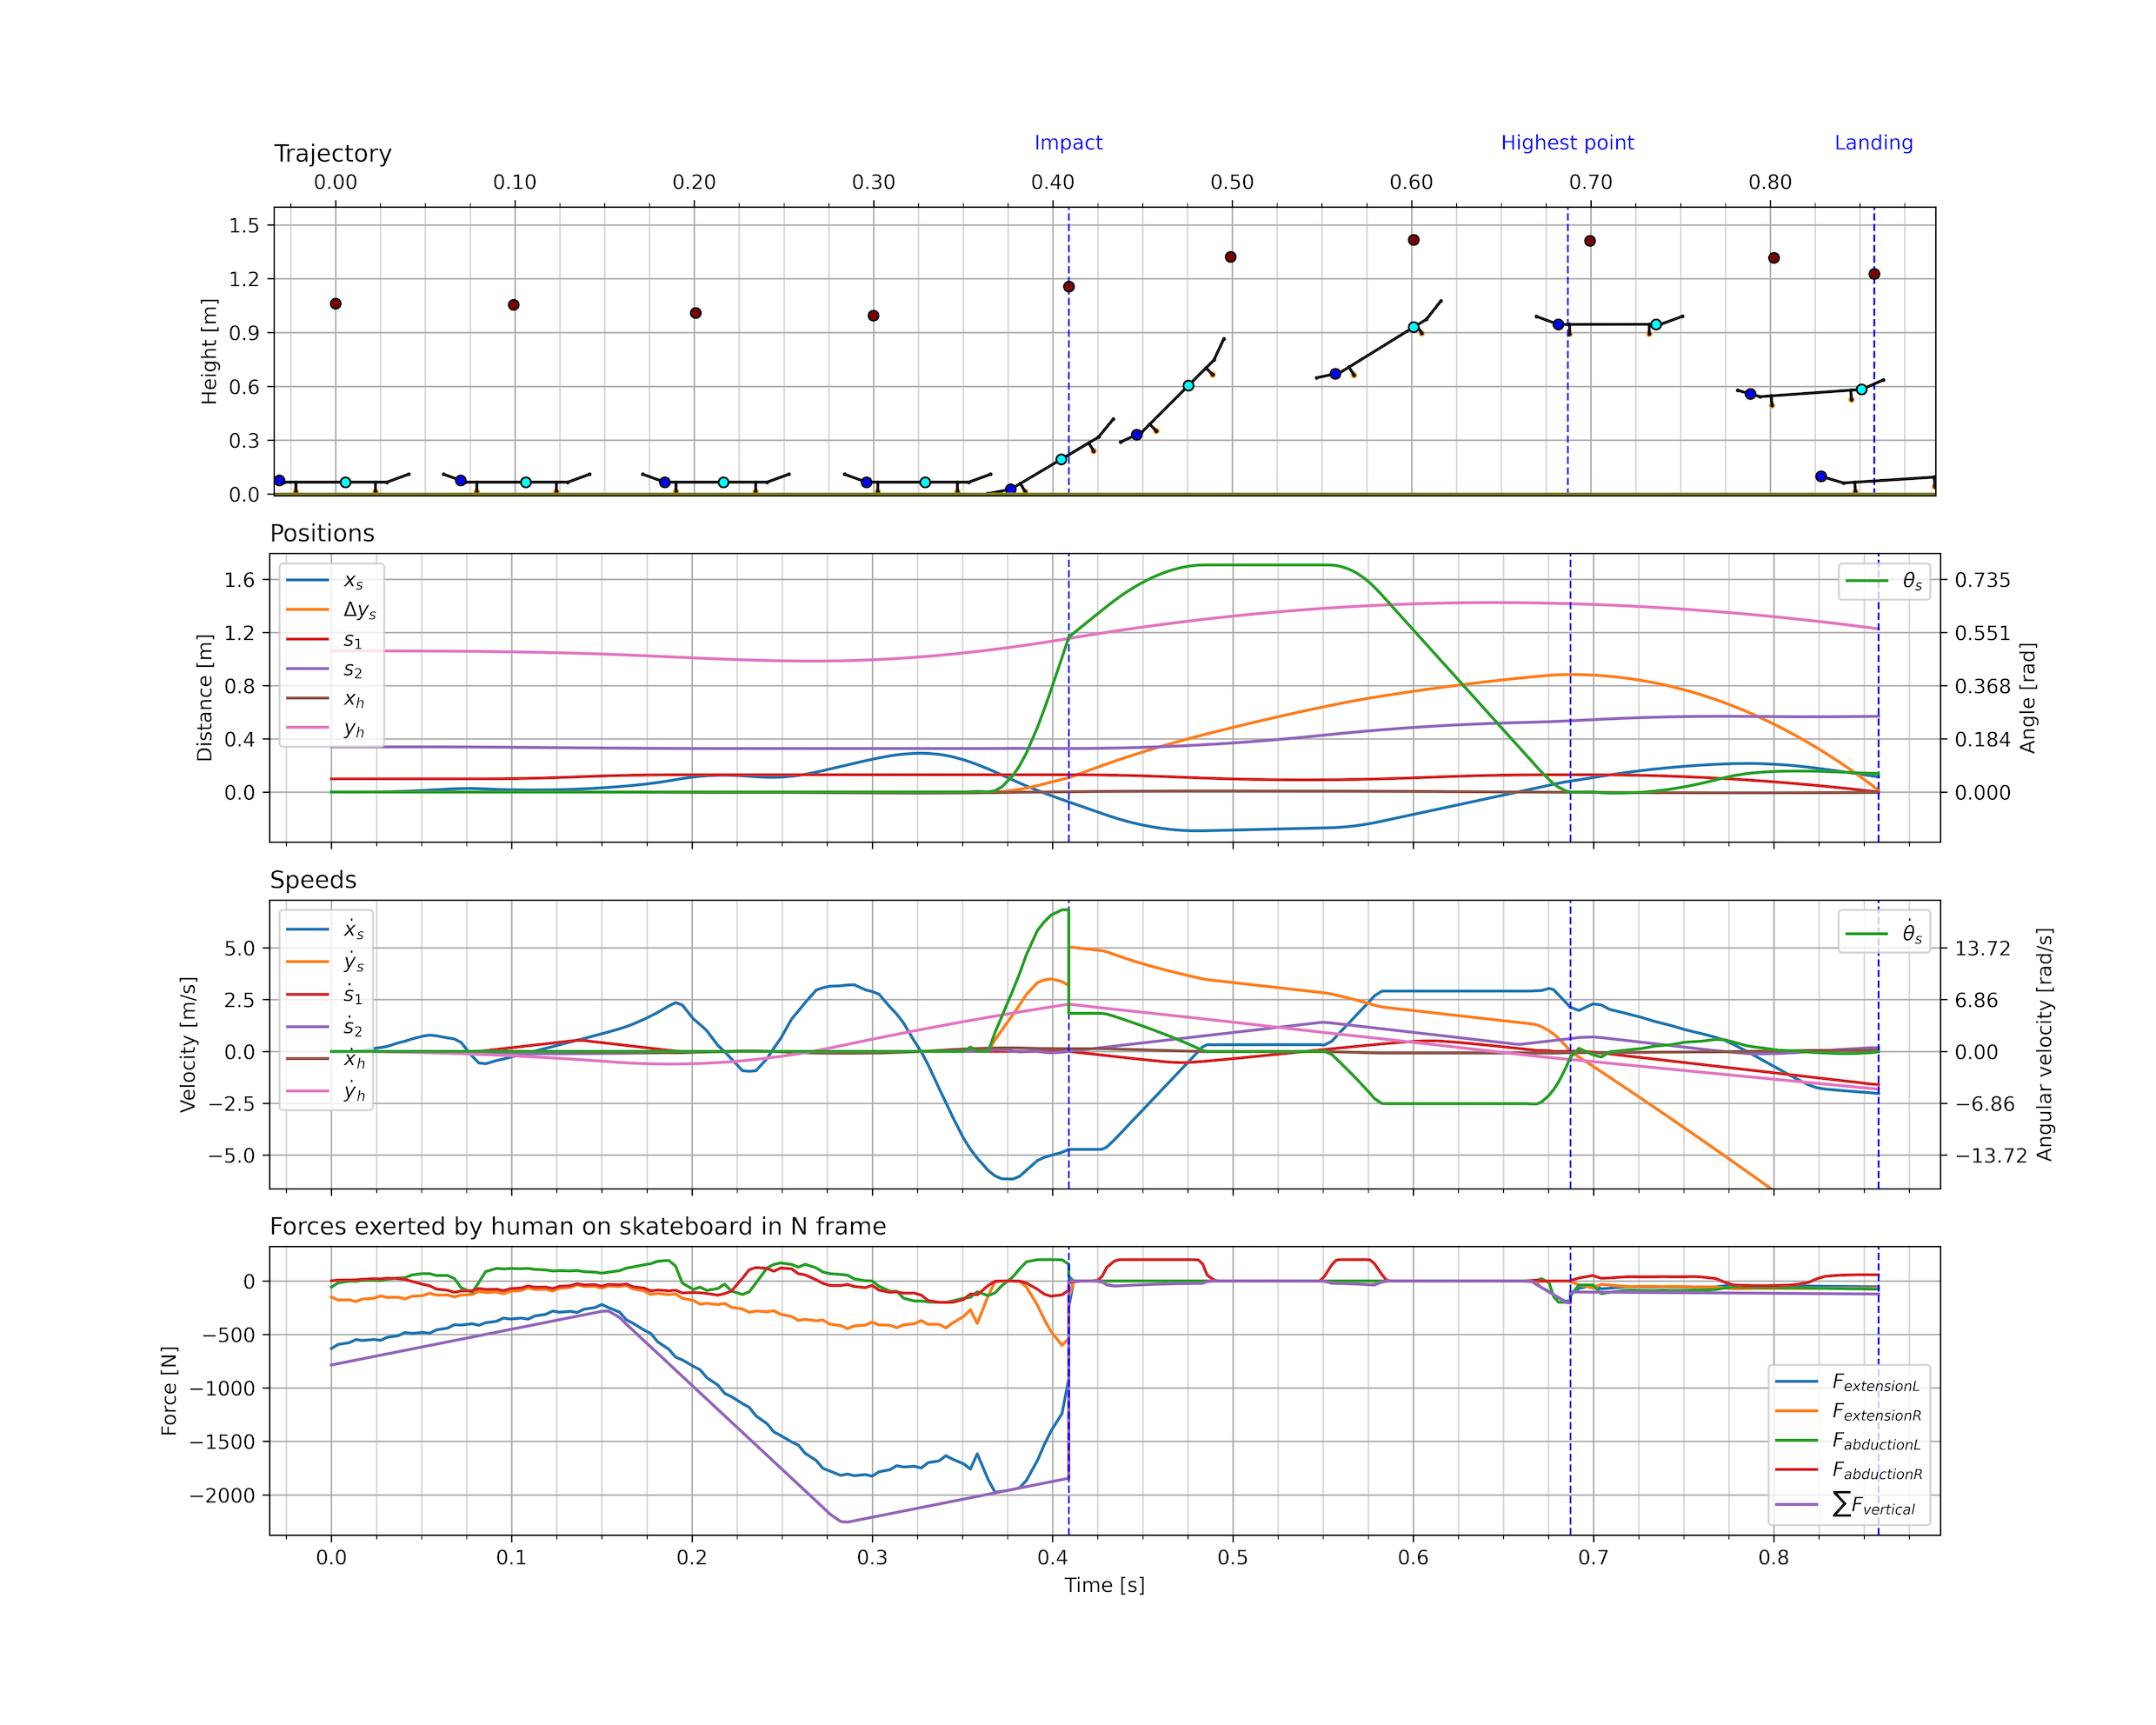
\includegraphics[trim={0cm 0cm 0cm 0cm},clip,width=0.8\textwidth]{figure/Results/data_r_wdpi600.png}}
    \newline
    \subfloat[Truck height]{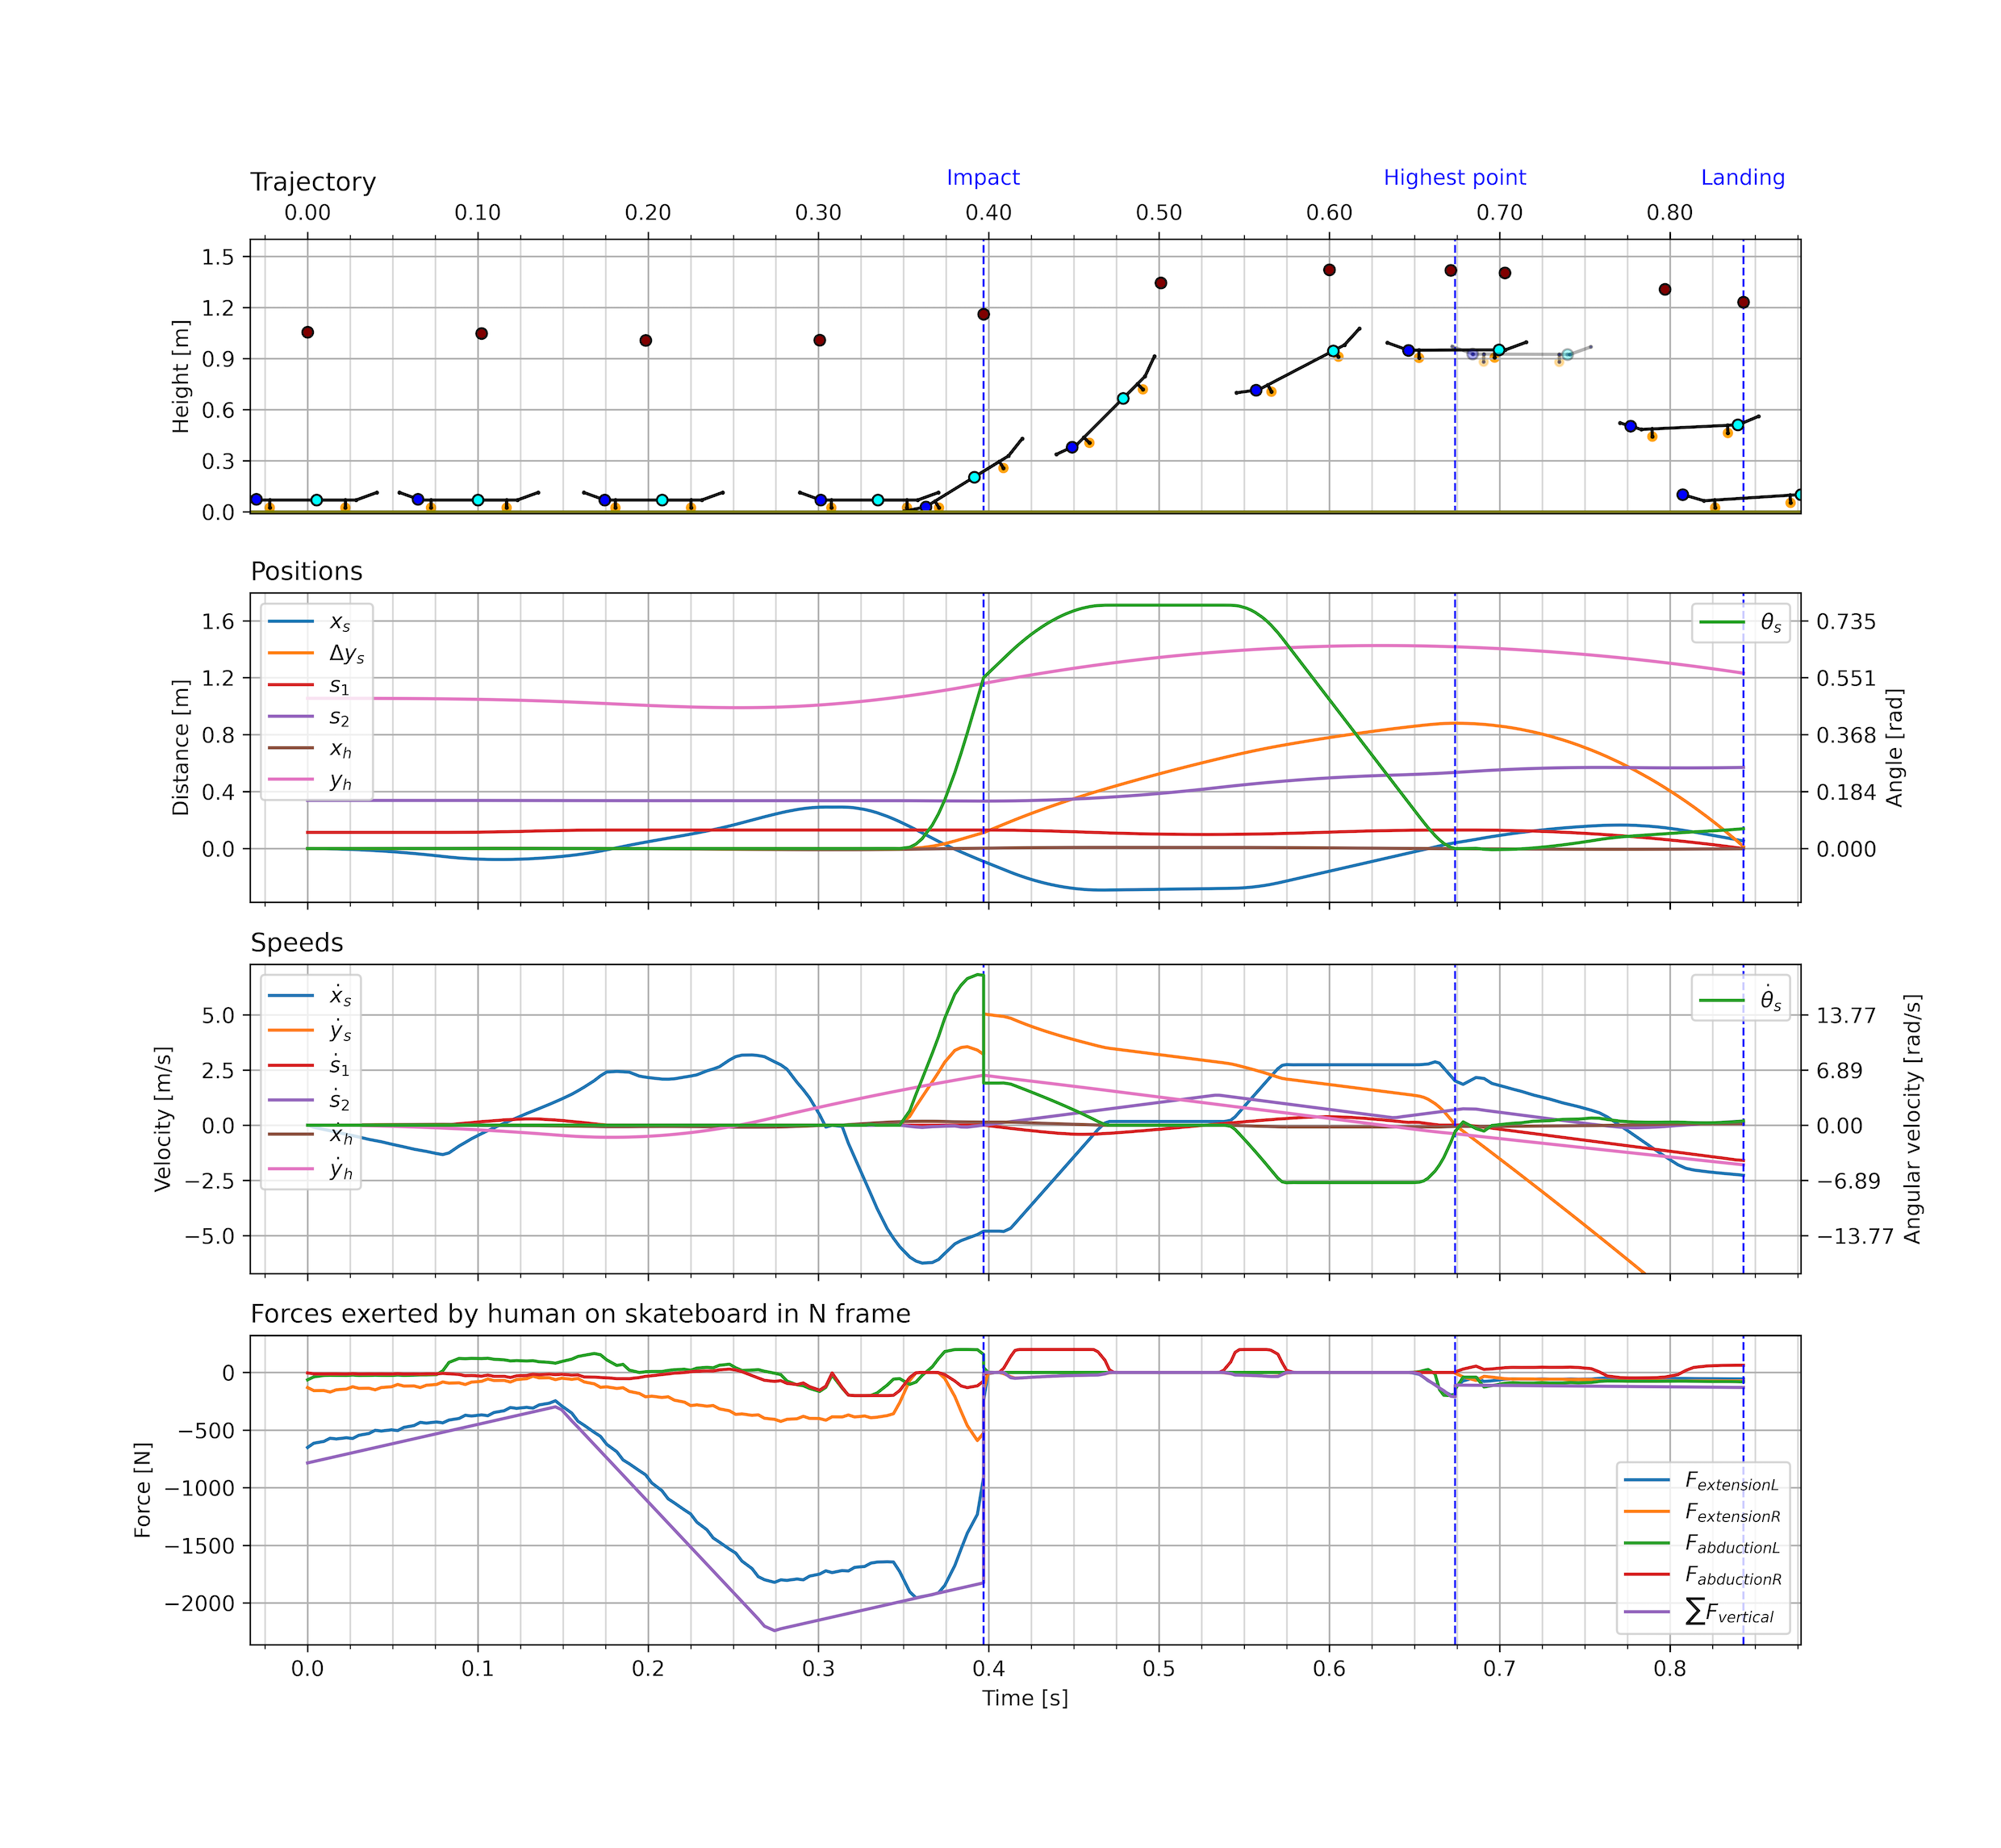
\includegraphics[trim={0cm 0cm 0cm 0cm},clip,width=0.8\textwidth]{figure/Results/data_d_trdpi600.png}}
    \caption{Wheel radius and truck height optimization results}    
\end{figure*}

% \begin{figure*}[b]    
%     \subfloat[Wheel radius]{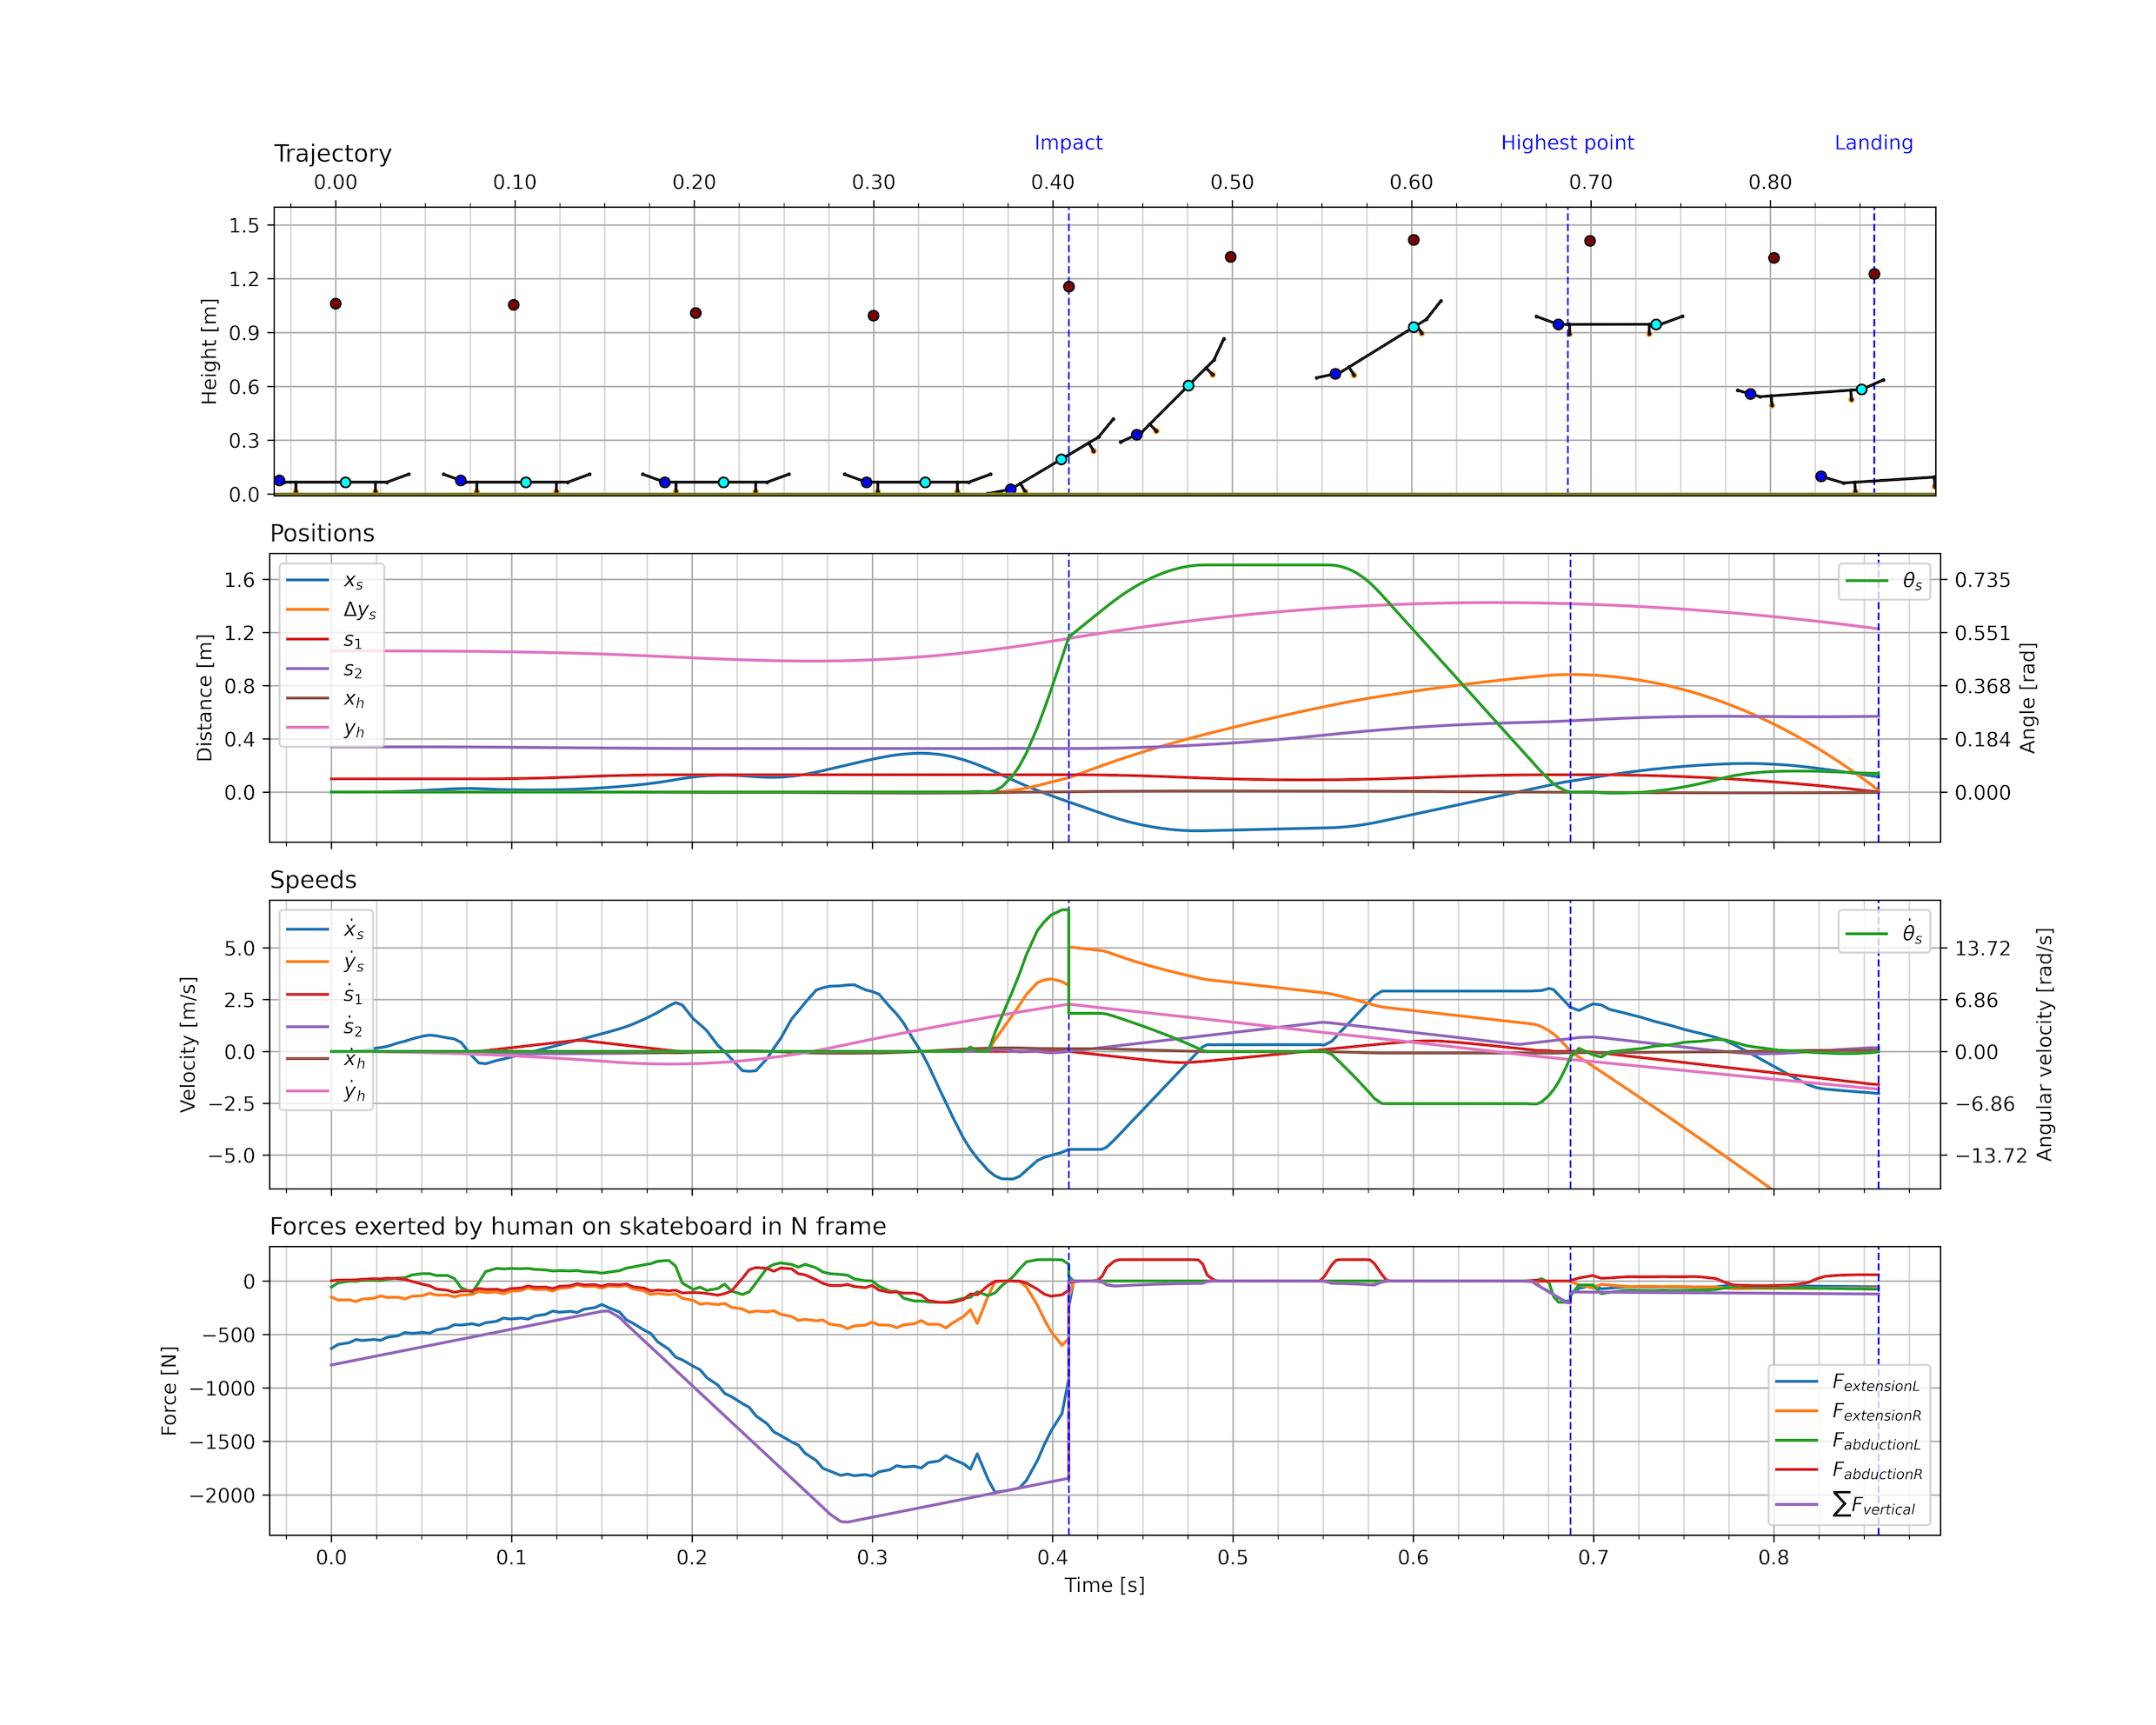
\includegraphics[trim={0cm 0cm 0cm 0cm},clip,width=0.8\textwidth]{figure/Results/data_r_wdpi600.png}}
%     \newline
%     \subfloat[Truck height]{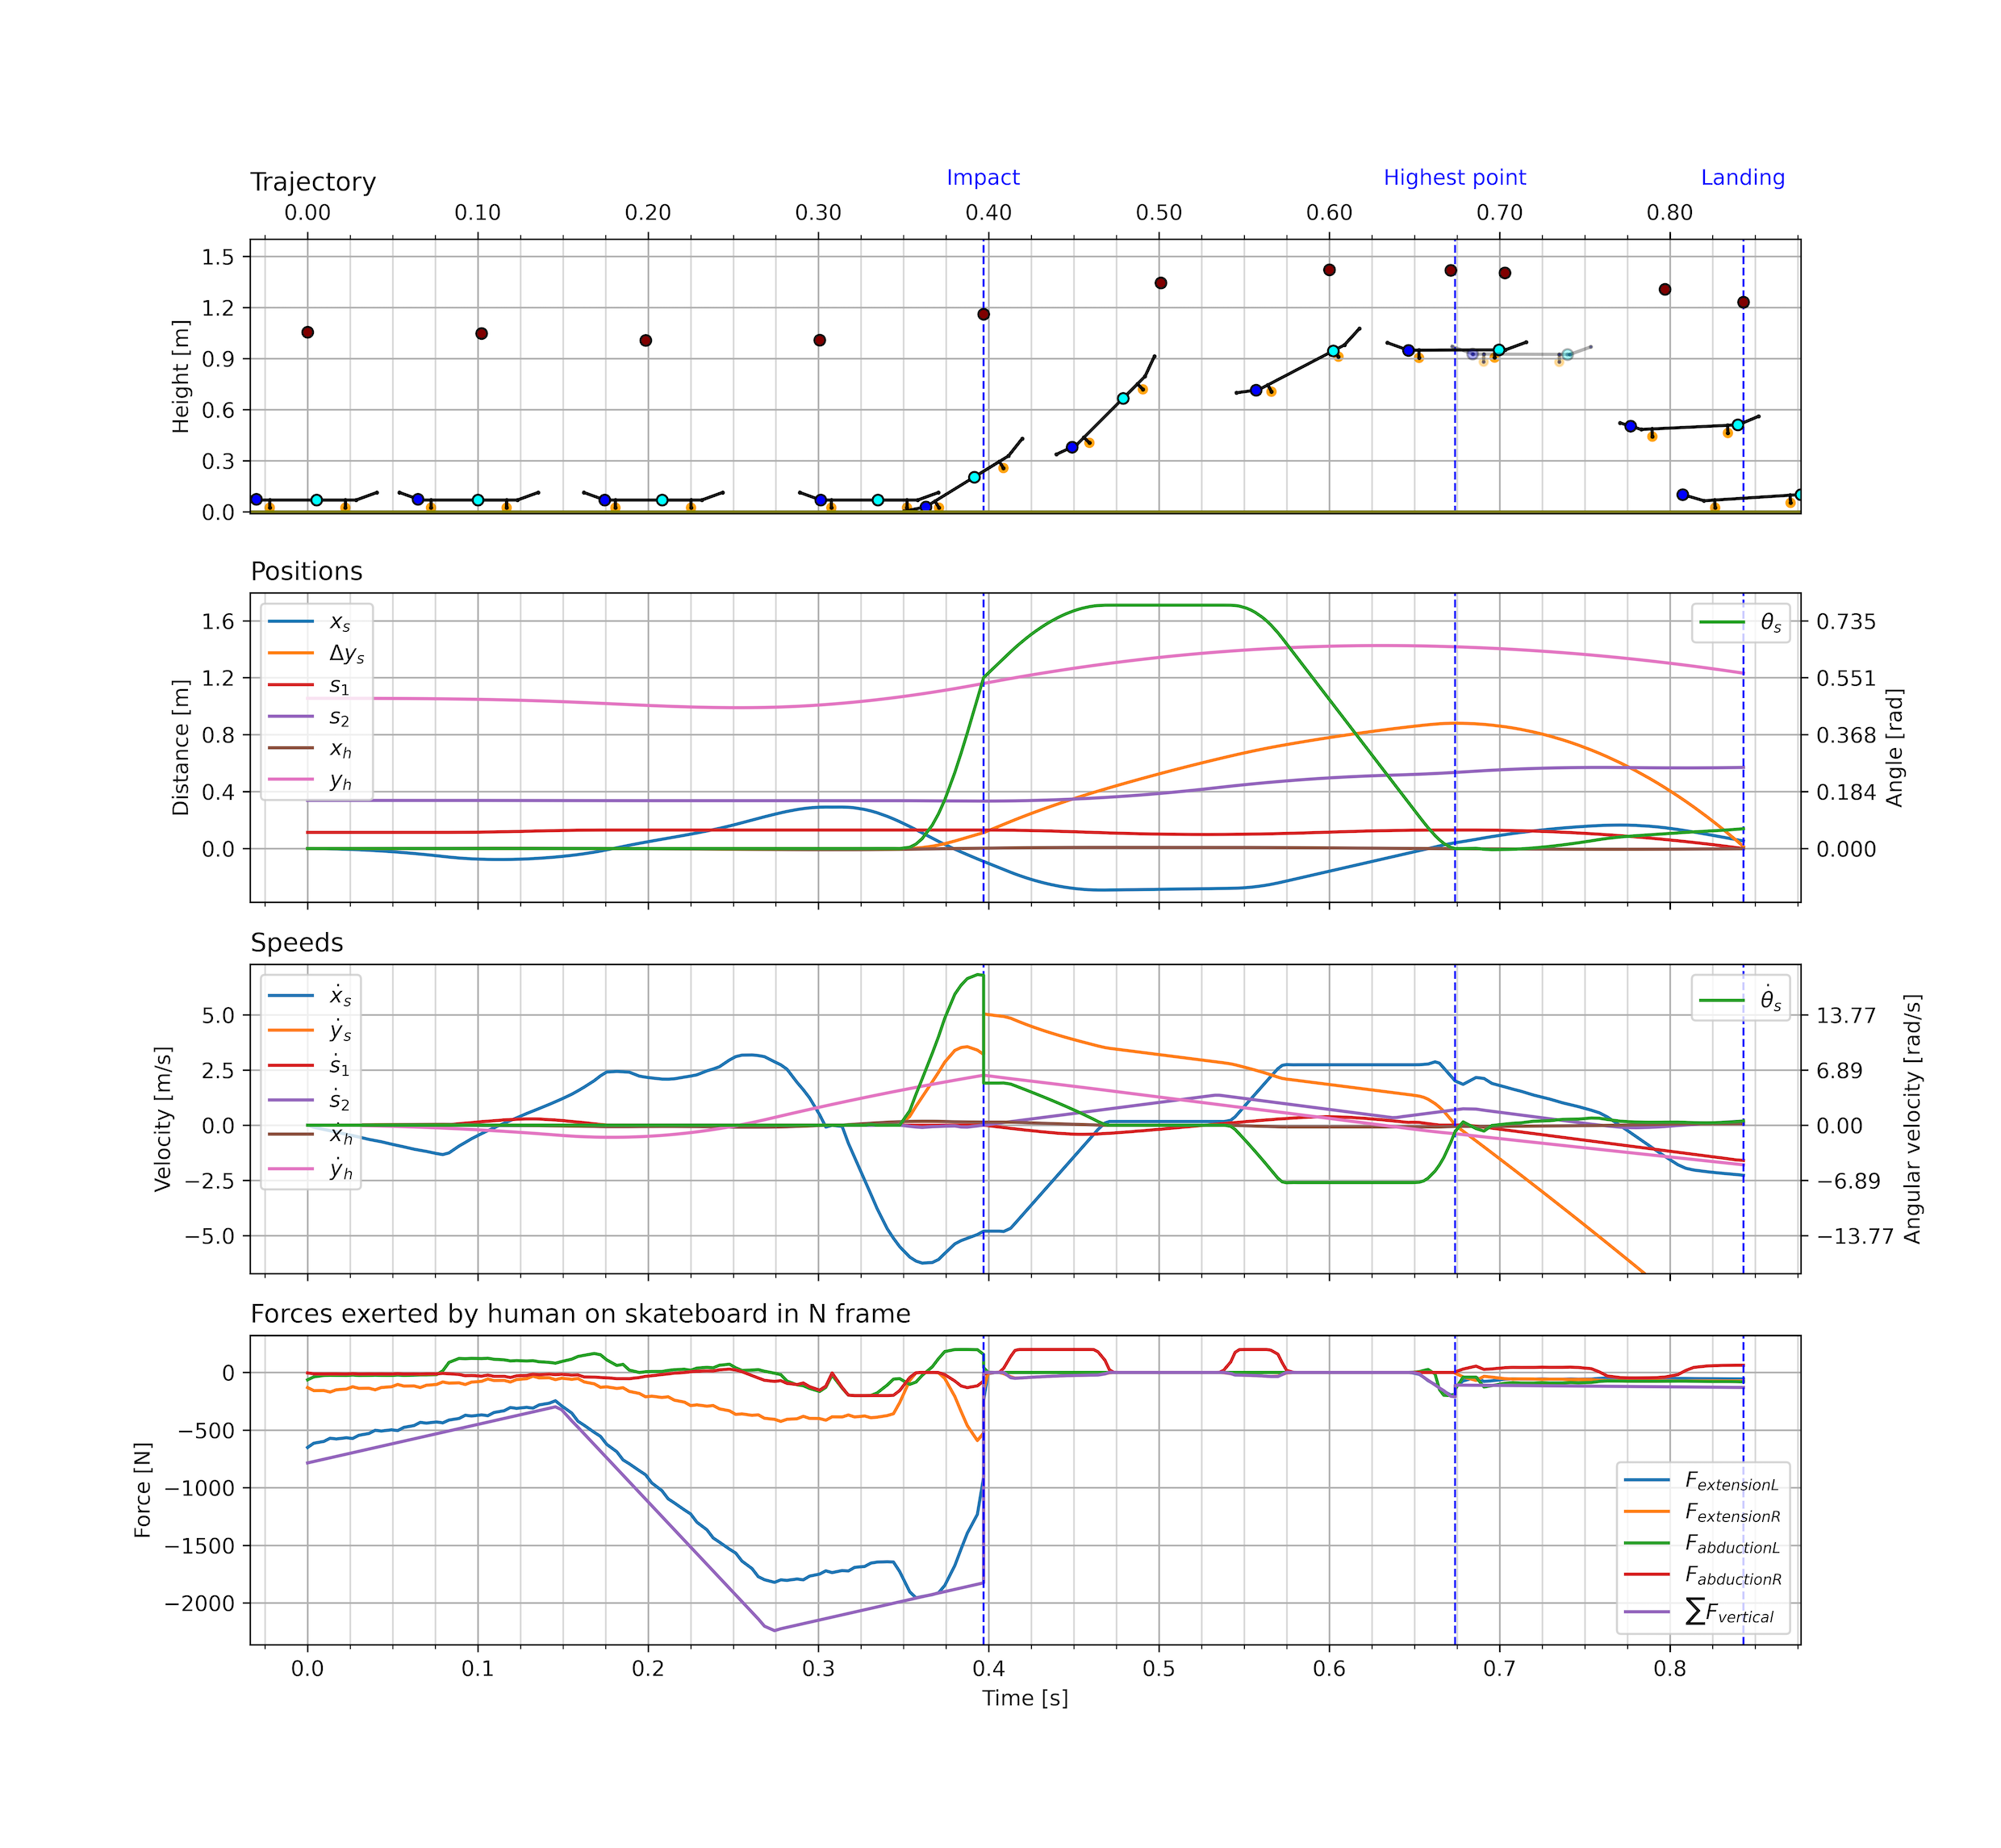
\includegraphics[trim={0cm 0cm 0cm 0cm},clip,width=0.8\textwidth]{figure/Results/data_d_trdpi600.png}}
%     \caption{Single parameter optimization}    
% \end{figure*}

\begin{figure*}[b]    
    \subfloat[Deck length]{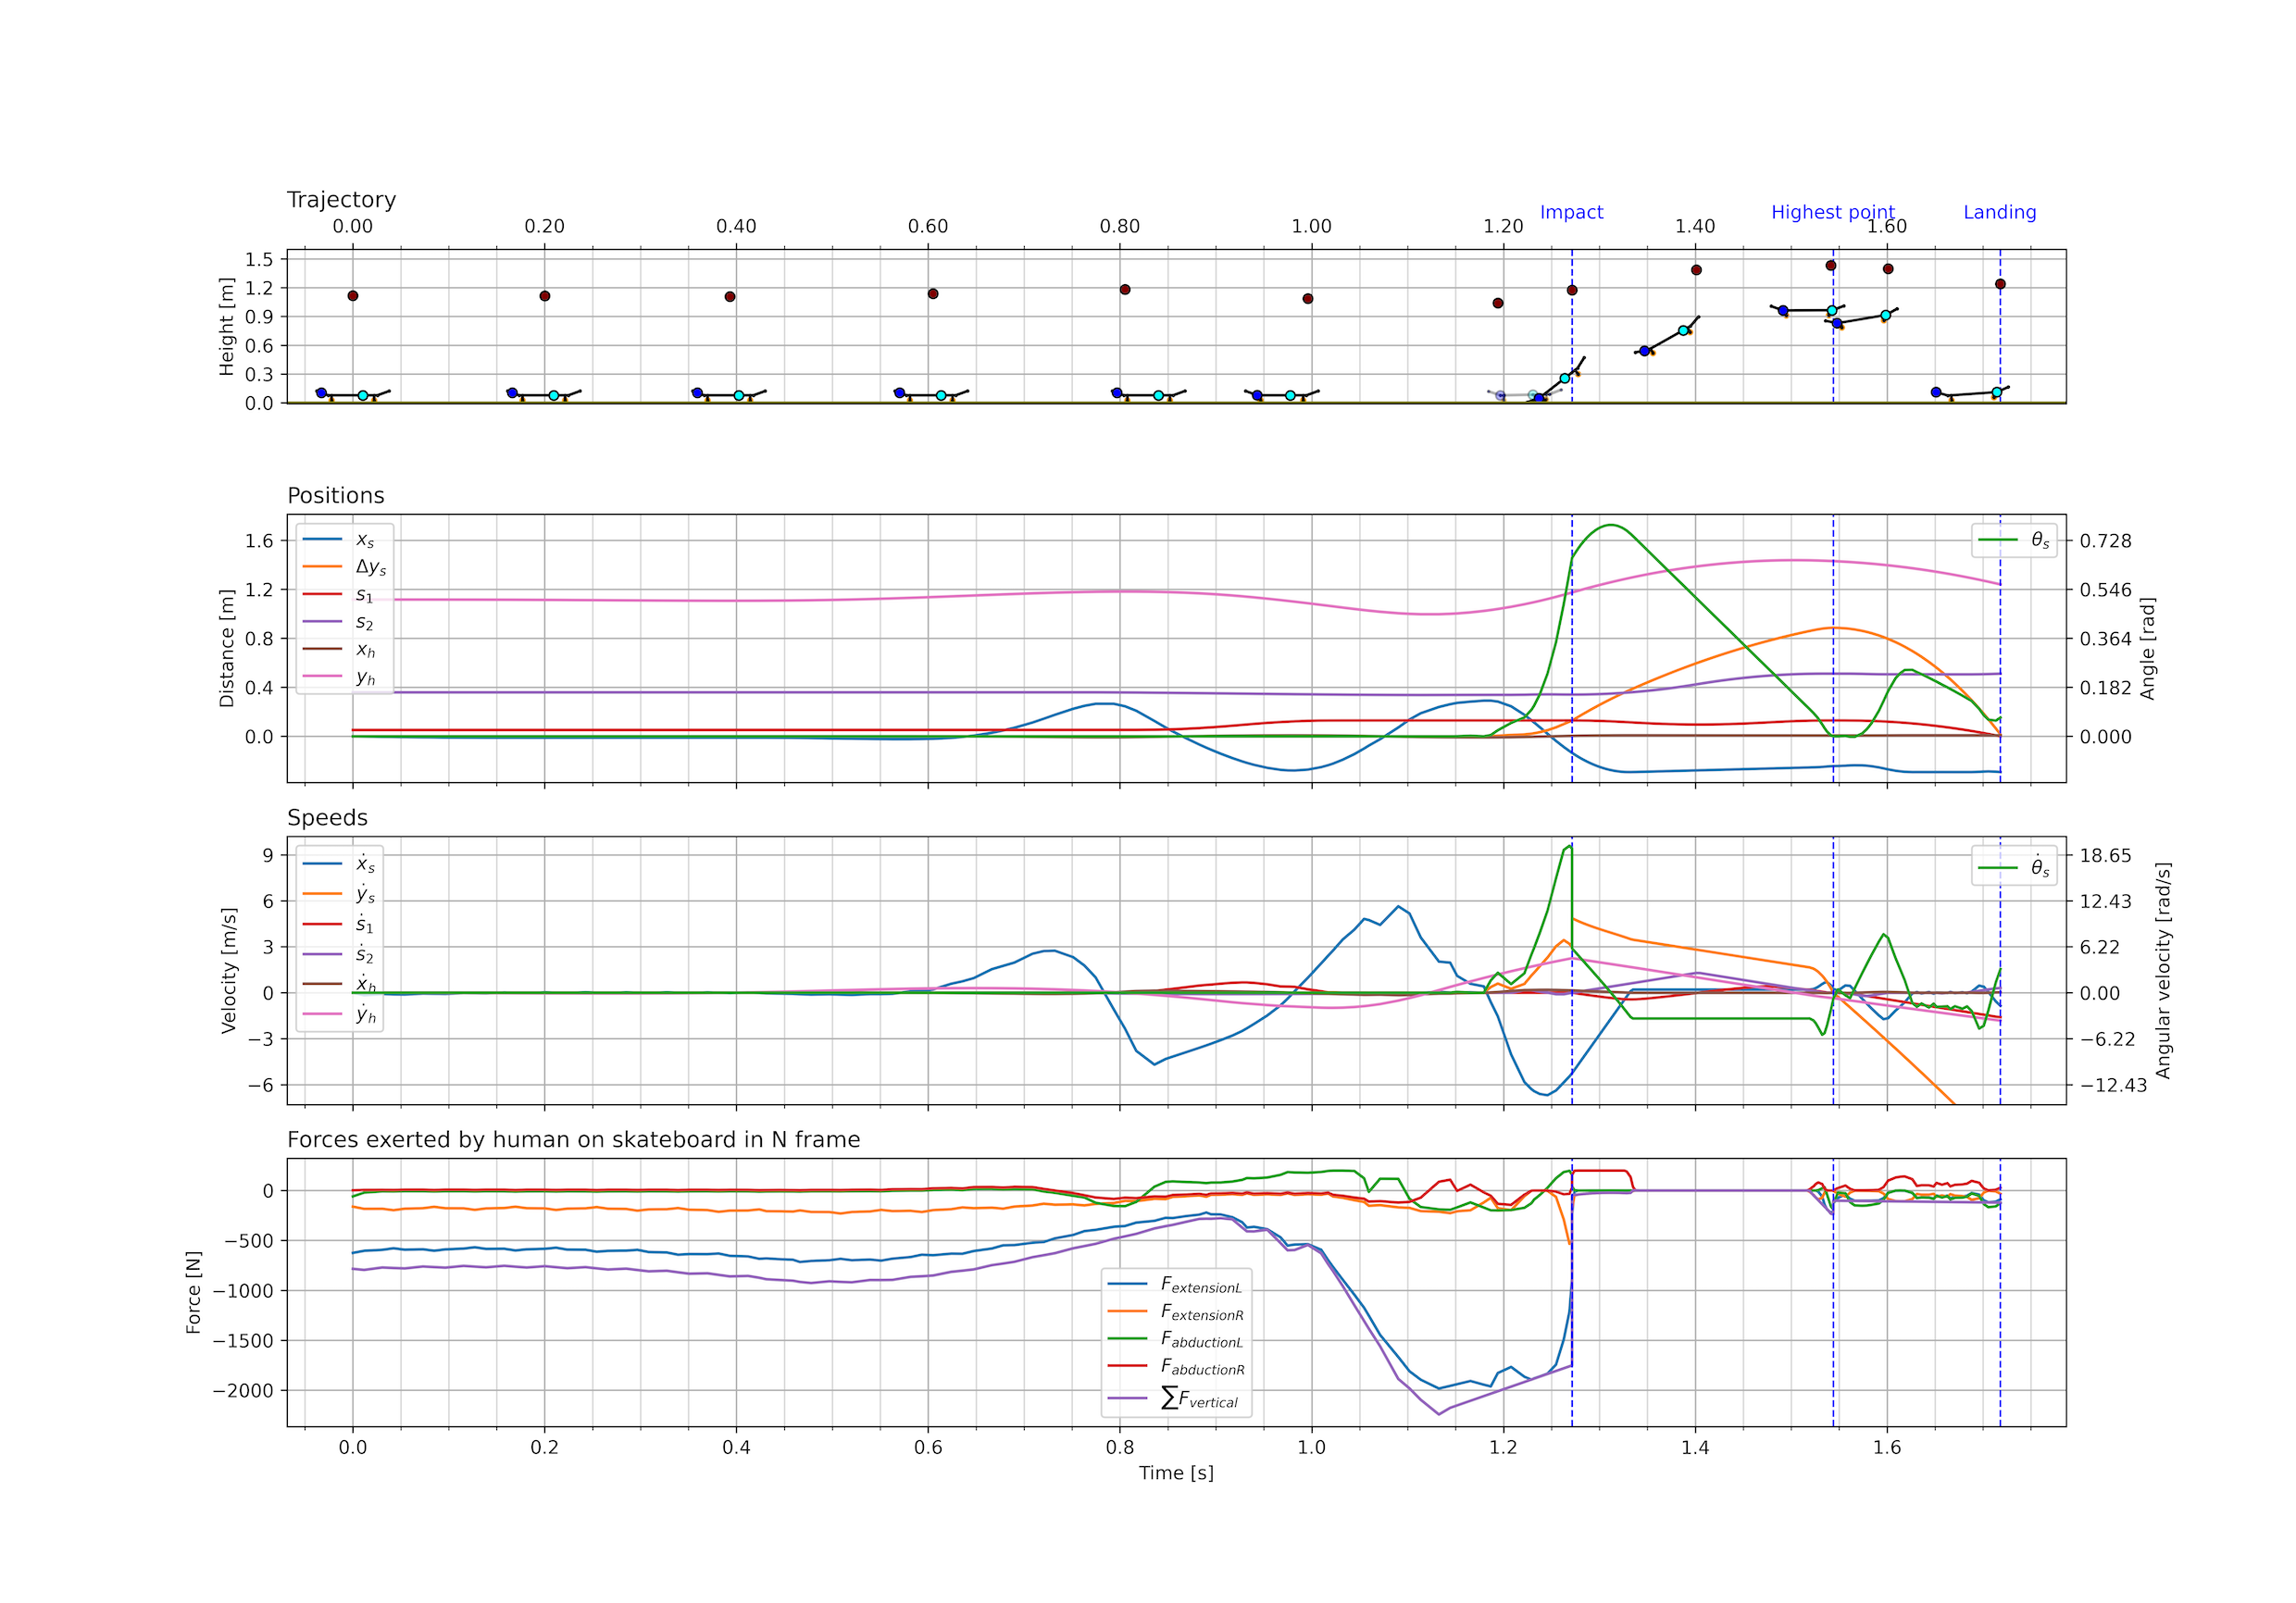
\includegraphics[trim={0cm 0cm 0cm 0cm},clip,width=0.8\textwidth]{figure/Results/data_l_fdpi600.png}}
    \newline
    \subfloat[Tail length]{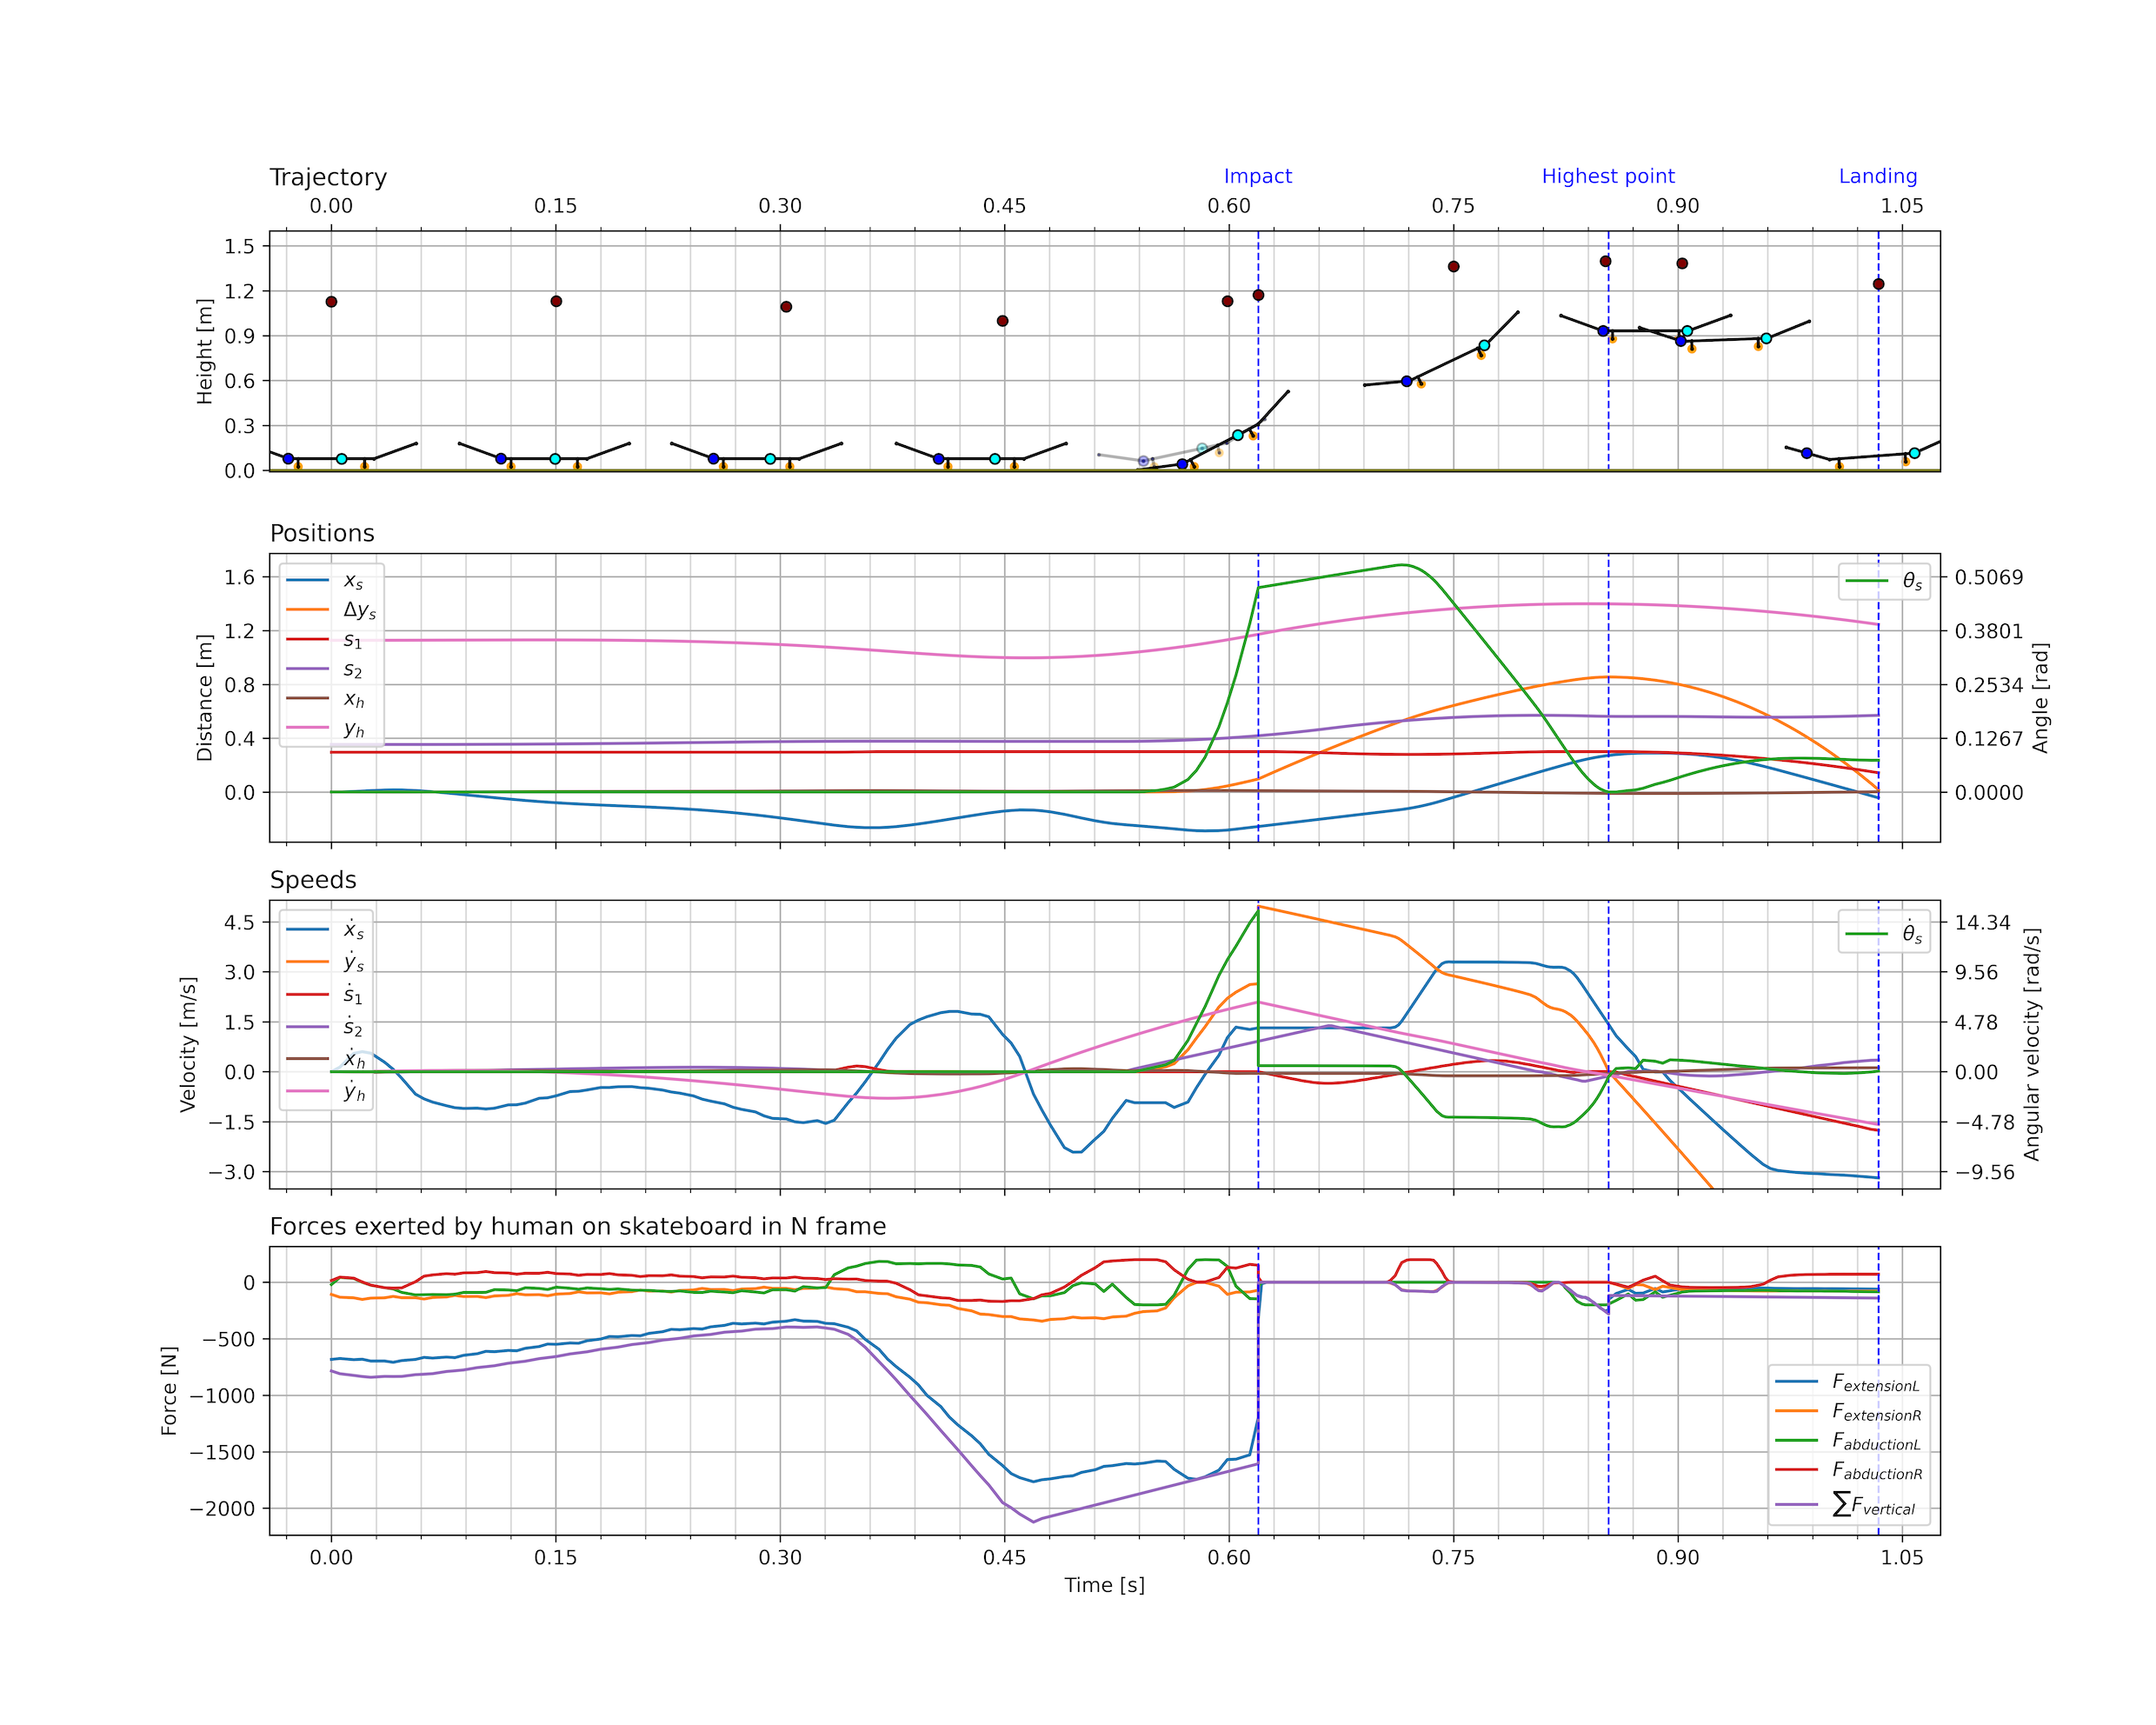
\includegraphics[trim={0cm 0cm 0cm 0cm},clip,width=0.8\textwidth]{figure/Results/data_l_tdpi600.png}}
    \caption{Deck length and tail length optimization results}    
\end{figure*}

\begin{figure*}[b]    
    \subfloat[Tail inclination]{\includegraphics[trim={0cm 0cm 0cm 0cm},clip,width=0.8\textwidth]{figure/Results/data_phidpi600.png}}
    \newline
    \subfloat[All parameters]{\includegraphics[trim={0cm 0cm 0cm 0cm},clip,width=0.8\textwidth]{figure/Results/data_alldpi600.png}}
    \caption{Tail inclination and all parameters optimization results}    
\end{figure*}


%Appendix will include inertia experiments and friction experiments

%% SHOW THAT NOSE ISN'T USED WHEN THE POSSIBILITY IS THERE

%% SHOW HOW VELOCITIES AFTER IMPACT ARE CALCULATED

%% SHOW 3 Friciton models
% During impact, friction can be present when there is a tangential velocity state relative to the impact surface. Poissons method and Newtons method have been shown unaccurate for such events and it is advised to use Stronge's method. This has been shown numerically in Stronge's comment on collision with friction\cite{stronge_comment_2010}. When the tail of the skateboard hits the ground, usually there is a tangential velocity state at the location of impact. This means that in real life a frictional impact occurs. Another implementation of the Poisson method during a frictional impact is solved with a set of constraints in the optimization\cite{patel_contact-implicit_2019}. The theory is that you create a variable $\phi(q_i)$, that represents the distance from the contact surface dependant on the generalized coordinates which should always be greater than 0. Furthermore there are three forces that should obey the friction cone presented in 

% \section*{Appendix B: Head of Second Appendix}
% \subsection*{Subsection head in appendix}
% The equation counter is not reset in an appendix and the numbers will
% follow one continual sequence from the beginning of the article to the very end as shown in the following example.

\end{document}
